\documentclass[sigconf,10pt]{acmart}
%\documentclass[letterpaper,twocolumn,10pt]{article}
% \usepackage{usenix-2020-09}
\usepackage{amsmath}
\usepackage{amsthm}

\usepackage{xfrac}
\usepackage{algorithm}
\usepackage[noend]{algpseudocode}
% \usepackage{times}
\usepackage{hyperref}
% \usepackage{subfig}
\usepackage{tikz}
\usetikzlibrary{math}
\usepackage{pgfplots}
\usetikzlibrary{pgfplots.groupplots}
\usepackage{pgfplotstable}
\usepackage[subtle]{savetrees}

% axis style, ticks, etc
\pgfplotsset{every axis/.append style={
                    label style={font=\footnotesize},
                    tick label style={font=\footnotesize}  
                    }}

\usepackage{caption}
\usepackage{subcaption}
\usepackage{multirow}
\usepackage{tabularx}
\usepackage{array}
\usepackage{xspace}

\newcolumntype{s}{>{\hsize=.3\hsize\linewidth=\hsize}X}
\newcolumntype{D}{>{\hsize=.3\hsize\linewidth=\hsize}X}
\newcommand{\wdImg}{\dimexpr \linewidth-2\tabcolsep} %width of the image

\hypersetup{pdfstartview=FitH,pdfpagelayout=SinglePage}

% \setlength\paperheight {11in}
% \setlength\paperwidth {8.5in}
% \setlength{\textwidth}{7in}
% \setlength{\textheight}{9.25in}
% \setlength{\oddsidemargin}{-.25in}
% \setlength{\evensidemargin}{-.25in}

\newcommand{\rg}[1]{\textcolor{blue}{(\textbf{GR:} #1)}}
\newcommand{\vk}[1]{\textcolor{green}{(\textbf{VA:} #1)}}

% \newtheorem{theorem}{Theorem}
% \newtheorem{definition}{Definition}
% \newtheorem{lemma}{Lemma}
\newtheorem{observation}{Observation}

% we have a big fig
\renewcommand{\floatpagefraction}{.8}%
% \renewcommand{\topfraction}{.8}
% \renewcommand{\bottomfraction}{.8}
\newcommand{\nftables}{\texttt{nftables}\xspace} 

% TODO: remove for the CR!
% \pagestyle{plain}
% \settopmatter{printfolios=true}

%% SIGCOMM
% Copyright
\renewcommand\footnotetextcopyrightpermission[1]{} % removes footnote with conference info
\setcopyright{none}
%\setcopyright{acmcopyright}
%\setcopyright{acmlicensed}
%\setcopyright{rightsretained}
%\setcopyright{usgov}
%\setcopyright{usgovmixed}
%\setcopyright{cagov}
%\setcopyright{cagovmixed}

\settopmatter{printacmref=false, printccs=false, printfolios=true}

% DOI
\acmDOI{}

% ISBN
\acmISBN{}

%Conference
%\acmConference[Submitted for review to SIGCOMM]{}
%\acmYear{2018}
%\copyrightyear{}

%% {} with no args suppresses printing of the price
\acmPrice{}

\begin{document}

% \conferenceinfo{HotNets 2022} {}
% \CopyrightYear{2022}
% \crdata{X}
% \date{}

%%%%%%%%%%%% THIS IS WHERE WE PUT IN THE TITLE AND AUTHORS %%%%%%%%%%%%

\title{More Bang for the Buck: Superlinear Scaling with Distributed Self-adjusting Systems}

\author{Paper \#619, 12 + 7 pages}
% \author{Jonas Köppeler, Maciej Pacut, Tamás Lévai, Vamsi Addanki, Stefan Schmid, Gábor Rétvári}

\begin{abstract}
  Conventional wisdom suggests that a linear increase of the number of workers in a distributed system can result in at most a linear performance improvement.  In this paper we show that distributed systems can be \emph{systematically} architected to achieve faster-than-linear (superlinear) scaling. Our insight is that dispatching jobs to parallel workers so that the locality of reference in the workers' input increases, and implementing the workers with a self-adjusting algorithm to take advantage of the higher locality, jointly yield superlinear scaling. We demonstrate the general applicability of our methodology in extensive simulations: scaling textbook self-adjusting algorithms we obtain 100--3,300x speedup using only 48 CPU cores (up to 70x beyond linear scaling). Then, we present two case studies. Using our architectural blueprint to scale a Memcached+PostgreSQL storage system we attain 35x speedup with 15 threads (2.3x above linear). Then we re-engineer the default Linux packet classifier to self-adjust with load, obtaining 800x speedup on synthetic traces and 220x speedup on real firewall traces with 32 CPU cores (5--25x times performance improvement compared to the vanilla Linux kernel).
\end{abstract}

\maketitle

% \tableofcontents

% a unique combination of \emph{locality-boosting load balancing} to spread load among workers implemented using \emph{self-adjusting data structures}.
  
\section{Introduction}\label{sec:introduction}

With the end of Moore's law, computing power in modern systems increasingly comes in the form of parallel processing resources.  A major obstacle faced by network engineers is how to harness this increasingly parallel computing power for scaling distributed systems \cite{265065, 10.5555/3307441.3307467, 10.1145/2815400.2815423, 10.1145/3098822.3098826, 10.5555/3154630.3154639}.

In horizontally scaled applications, a load balancer dispatches jobs across a fleet of workers that process the jobs in parallel \cite{10.5555/3235491}.  In the context of \emph{web applications}, HTTP load balancers \cite{194966, 211279, 9552525} distribute requests across a swarm of backend web servers.  % by hashing over the source IP address (``sticky sessions'').
% This way, requests from the same client will hit the same backend server, improving request locality.
% Meanwhile, resource state is maintained in a key-value store or a relational database.
Multicore \emph{OS network stacks} \cite{211263, 10.1145/3359989.3365412, 10.1145/3452296.3472914} run multiple instances of the networking logic on different CPUs and leverage the NIC to dispatch packets to CPU cores. % In order to avoid packet reordering and improve CPU cache performance, the NIC typically computes a hash over the packet header fields to select the CPU (RSS, RPS, etc.).
In massive-scale \emph{key-value stores} \cite{ghigoff2021bmc}, the key-space is hashed into multiple shards (partitions) and each shard is assigned to a separate server for processing.  The system's overall goal is to achieve the greatest possible parallel speedup with a given number of workers, in order to minimize the execution time of a single task or maximize the number of completed tasks in a given time period.

Suppose a web app handles 100 requests per second using a single server. As we add another server, we expect a throughput of 200 requests per second. In reality, however, we usually obtain slightly less, and this is worsened as the system is scaled up further. This is because some fraction of most workloads is inherently sequential and, therefore, bound to execute on a single CPU core. For instance, the web servers may need to synchronize on a mutex to access global state, which makes all state updates sequential.  Beyond a certain threshold parallel performance plateaus as the sequential workload becomes a bottleneck.

The maximum speedup, measured as the ratio of the wall clock times of sequential and parallel execution, is formally described by Amdahl's law \cite{10.1145/1465482.1465560}. In general, the greater the sequential portion compared to the parallelizable fraction of the code, the more performance is lost compared to an ``ideal'' linear scaling, and the faster the system reaches saturation (see Fig.~\ref{fig:amdahl}). Amdahl's law is a cornerstone result in the parallel and high-performance computing practice and, despite often being debated \cite{10.1145/42411.42415}, extended \cite{4563876, 6280307,1580395,406581,6163449}, and misused \cite{10.5555/775339.775386}, it has remained one of the most useful tools in the system engineering toolbox \cite{10.5555/1951599}.

\begin{figure}[t]
  \centering
  % \includegraphics[width=0.8\linewidth]{fig/usl.png}
  \begin{small}
  \begin{small}
  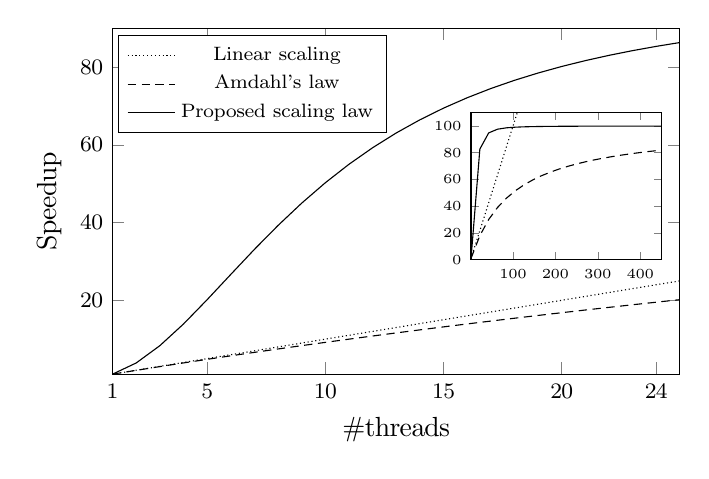
\begin{tikzpicture}[remember picture]
    \begin{axis}[
      width=250pt,
      height=170pt,
      xlabel={\#threads},
      ylabel={Speedup},
      xlabel near ticks,
      ylabel near ticks,
      xmin=1,
      xmax=25,
      ymin=1,
      ymax=90,
      xtick={1,5,10,15,20,24},
      legend style = {
        anchor = north west,
        at = {(rel axis cs:0.01,0.98)},
        font=\scriptsize,
        % draw = none,
      },
      no markers
      ]
      % use TeX as calculator:
      \addplot[domain=1:25,black,densely dotted]{x};
      \addlegendentry{Linear scaling}

      \addplot[domain=1:25,black,densely dashed]{1/(0.01 + (1-0.01)/x)};
      \addlegendentry{Amdahl's law}

      \addplot[domain=1:25,black,solid]{1/(0.01 + (1-0.01)/x^2)};
      \addlegendentry{Proposed scaling law}

      \coordinate (insetPosition) at (rel axis cs:.97,0.25);
      % \addplot[domain=0:15,black,loosely dashed]{1/(0.4 + (1-0.4)/x)};
      % \addlegendentry{Amdahl's law ($\delta=0.4$)}

      % \addplot[domain=0:15,black,loosely dotted]{1/(0.4 + (1-0.4)/x^2)};
      % \addlegendentry{Proposed scaling law for MTF ($\delta=0.4$)}
    \end{axis}
    \begin{axis}[
      at={(insetPosition)},
      anchor={outer south east},
      width=105pt,
      height=85pt,
      tiny,
      % xlabel={\#cores},
      % ylabel={Speedup},
      xmin=1,
      xmax=450,
      ymin=0,
      ymax=110,
      % ytick={1,2,3,4,5},
      no markers]
      \addplot[domain=1:500,black,densely dotted]{x};
      \addplot[domain=1:500,black,densely dashed]{1/(0.01 + (1-0.01)/x)};
      \addplot[domain=1:500,black,solid]{1/(0.01 + (1-0.01)/x^2)};
    \end{axis}
  \end{tikzpicture}
\end{small}

%%% Local Variables:
%%% mode: latex
%%% TeX-master: "../distributed_mrf.tex"
%%% End:

\end{small}
  \caption{Linear scaling, Amdahl's law and the superlinear scaling ($s=0.01$). The inset shows the asymptotics.}
  \label{fig:amdahl}
\end{figure}

Inherent to Amdahl's law is that no system can scale faster than linear: doubling parallel resources will yield at most two times the performance. Curiously, there have been several reports on faster-than-linear (\emph{superlinear}) scaling experimentally observed in, e.g., database systems \cite{scalability-analyzed, 10.5555/1012889.1012894}, distributed caching \cite{271208, dobb-2}, SDN analytics \cite{sdn-analytitcs}, high-performance computing \cite{556383, 7733347, 6483679}, multi-robot systems \cite{10.1007/978-3-319-77610-1}, and parallel search in information retrieval systems \cite{dobb-1, dobb-2} (see full taxonomies in \cite{7733347, 80148}).
% There seem to be two ways to achieve such superlinear speedup \cite{7733347, 80148}: do disproportionately less work in each worker as we scale the system \cite{7733347}, or add more resources per thread \cite{80148}.
% One typical context in which superlinear growth often emerges is distributed caching \cite{271208, 10.5555/1012889.1012894, dobb-2}: the more CPU cores the more (unshared) L1 cache space available to the application, which tends to make memory-bound\slash cache-bound code disproportionately faster \cite{80148} (see an analysis in \S\ref{sec:background}).  
Many authors argue, however, that superlinear scaling is merely a byproduct of running memory-\slash cache-bound applications on a ``bigger machine'' \cite{80148}, others are concerned that it is hard to generalize beyond a specific set use cases \cite{7733347, 80148}, and some outright dismiss faster-than-linear scaling all together \cite{gunther-hotsos, 10.1016/0167-8191(86)90024-4}, concluding that \emph{``superlinearity, although alluring, is as illusory as perpetual motion''} \cite{10.1145/2773212.2789974}.

In this paper we challenge this view: we show that distributed systems can be methodologically designed for reaching superlinear scaling. Our motivation is that networking applications are often embarrassingly parallel, % with little or no dependency between parallel workers,
which may admit a massive superlinear initial growth phase before scaling eventually and unavoidably blocking on a serial bottleneck.

Our main observation is that, to achieve superlinearity, one has to carefully combine an appropriate load balancing policy with a proper worker implementation. Indeed, load balancing in most distributed systems is deliberately designed to improve the locality of reference in the input of the workers: web apps apply the ``sticky sessions'' rule to route all requests of a particular user to the same web server; %, rendering subsequent requests faster by having all per-user state available locally;
networking code often uses IP 5-tuple hashing on the NIC to ensure that all packets of a flow are processed on the same CPU; % that has local access to per-flow information;
and key-hashing in sharded key-value stores directs all client queries to a key to the same replica. Each of these load balancing policies tend to make the input stream processed by the parallel workers more predictable, compared to the input processed by the system. Such a \emph{locality boosting load balancer}, paired with a \emph{self-adjusting algorithm} so that workers can take advantage of the higher input predictability to adaptively improve their performance, will, as we show both theoretically and empirically, yield faster-than-linear speedup in a broad range of applications (see Fig.~\ref{fig:amdahl}). % One growth factor would come from the self-adjusting algorithm becoming proportionately faster as it processes a smaller and smaller subset of the inputs, and another factor would result from the fact that we throw more CPU resources to the system.

After some background on Amdahl's law (\S\ref{sec:background}), we present our \emph{distributed self-adjusting system architecture} and show that superlinear speedup is a natural product of combining locality-boosting load balancing with self-adjusting algorithms (\S\ref{sec:architecture}). Using common list and tree search algorithms from the literature, we achieve 100x--3300x speedup in simulations, orders of magnitude surpassing Amdahl's law or even plain, linear scaling. As an unexpected byproduct, we attain linear scaling even when we limit the system to a single CPU core. Then we extend our analysis to real systems (\S\ref{sec:case-study}): we carefully apply our methodology to engineer a Linux-kernel based packet classifier to reach superlinear scaling. On synthetic and real-life firewall traces, our implementation shows up to $800\times$ faster than linear scaling, $5\times$--$25\times$ improvement beyond the default Linux firewall implementation which scales according to Amdahl's law. Finally, we review related work (\S\ref{sec:related-work}) and draw the conclusions (\S\ref{sec:conclusions}). We note that all code will be available as open source after publication.

%%% Local Variables:
%%% mode: latex
%%% TeX-master: "distributed_mrf"
%%% End:



% !TEX ROOT = ./distributed_mrf.tex
\section{Background}\label{sec:background}

\begin{figure}[t]
  \centering
  \begin{small}
    \begin{small}
  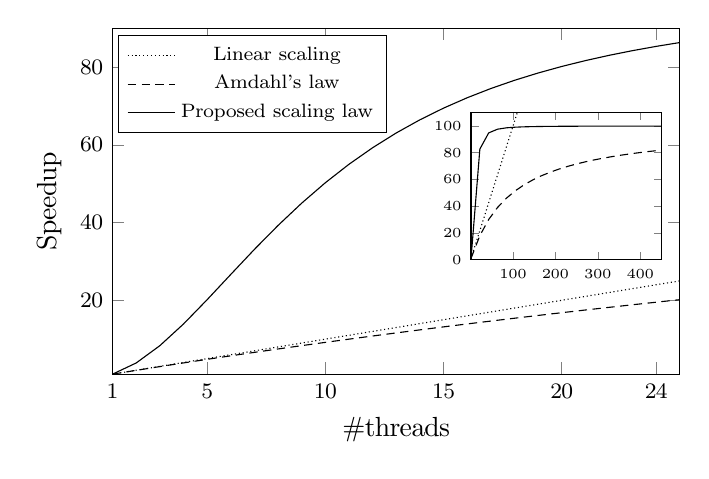
\begin{tikzpicture}[remember picture]
    \begin{axis}[
      width=250pt,
      height=170pt,
      xlabel={\#threads},
      ylabel={Speedup},
      xlabel near ticks,
      ylabel near ticks,
      xmin=1,
      xmax=25,
      ymin=1,
      ymax=90,
      xtick={1,5,10,15,20,24},
      legend style = {
        anchor = north west,
        at = {(rel axis cs:0.01,0.98)},
        font=\scriptsize,
        % draw = none,
      },
      no markers
      ]
      % use TeX as calculator:
      \addplot[domain=1:25,black,densely dotted]{x};
      \addlegendentry{Linear scaling}

      \addplot[domain=1:25,black,densely dashed]{1/(0.01 + (1-0.01)/x)};
      \addlegendentry{Amdahl's law}

      \addplot[domain=1:25,black,solid]{1/(0.01 + (1-0.01)/x^2)};
      \addlegendentry{Proposed scaling law}

      \coordinate (insetPosition) at (rel axis cs:.97,0.25);
      % \addplot[domain=0:15,black,loosely dashed]{1/(0.4 + (1-0.4)/x)};
      % \addlegendentry{Amdahl's law ($\delta=0.4$)}

      % \addplot[domain=0:15,black,loosely dotted]{1/(0.4 + (1-0.4)/x^2)};
      % \addlegendentry{Proposed scaling law for MTF ($\delta=0.4$)}
    \end{axis}
    \begin{axis}[
      at={(insetPosition)},
      anchor={outer south east},
      width=105pt,
      height=85pt,
      tiny,
      % xlabel={\#cores},
      % ylabel={Speedup},
      xmin=1,
      xmax=450,
      ymin=0,
      ymax=110,
      % ytick={1,2,3,4,5},
      no markers]
      \addplot[domain=1:500,black,densely dotted]{x};
      \addplot[domain=1:500,black,densely dashed]{1/(0.01 + (1-0.01)/x)};
      \addplot[domain=1:500,black,solid]{1/(0.01 + (1-0.01)/x^2)};
    \end{axis}
  \end{tikzpicture}
\end{small}

%%% Local Variables:
%%% mode: latex
%%% TeX-master: "../distributed_mrf.tex"
%%% End:

  \end{small}
  \caption{Linear scaling, Amdahl's law and superlinear scaling ($s=0.01$). The inset shows the asymptotics.}
    \label{fig:amdahl}
\end{figure}

There is an extensive background on scaling laws for characterizing the performance of a parallel system as a function of the computing\slash storage capacity available to it. In the following, we will use the terms ``distributed'' and ``parallel'' interchangeably to connote a networked system scaled to multiple independent compute threads (``workers''), e.g., scaled to parallel CPUs of the same node, distributed to separate nodes, run in multiple datacenters, etc.

A cornerstone result in parallel computing, Amdahl's law \cite{10.1145/1465482.1465560} establishes a firm limit on the performance gain one can obtain by distributing a computation task over multiple processors. Given a partially parallel program, denote the fraction of execution time spent in the sequential part of the code by $s$, and the parallel fraction by $(1-s)$. Here, some code is ``sequential'' if it cannot benefit from the improvement of parallel computing resources, like single-threaded code, critical sections guarded by exclusion locks, etc. Denote by $T(k)$ the runtime (in seconds) of the program when executed on $k$ processors, and let $S(k)=\frac{T(1)}{T(k)}$ denote the performance improvement relative to a single-threaded execution (i.e., the \emph{speedup}). Then, the following holds (see Fig.~\ref{fig:amdahl}):
\begin{equation}\label{eq:amdahl}
S(k) = \frac{T(1)}{T(k)} = \frac{1}{s + \frac{1-s}{k}} \enspace .
\end{equation}

Here, $\frac{1-s}{k}$ establishes that the perfectly parallel part of the program executes $k$ times faster on $k$ processors than on a single core. By Amdahl's law, \emph{(i)} no code can scale faster than linear (i.e., $\frac{d S(k)}{d k} \le 1$, with equality exactly when $s=0$), \emph{(ii)} throwing additional workers on a computation task yields diminishing returns ($\frac{d S(k)}{d k}$ is monotonically decreasing in $k$) and \emph{(iii)} the asymptotics is limited by the sequential part only ($\lim_{k\to \infty}S(k) = \frac1{s}$). For different applications and extensions of Amdahl's law, see \cite{4563876, 6280307,1580395,406581,6163449, 10.5555/1951599}.

Curiously, there have been several reports from a broad range of applications indicating faster-than-linear scaling, e.g., database systems \cite{scalability-analyzed, 10.5555/1012889.1012894}, distributed storage systems \cite{271208, dobb-2, icsoft20}, SDN analytics \cite{sdn-analytitcs}, high-performance computing applications \cite{556383, 7733347, 6483679}, multi-robot systems \cite{10.1007/978-3-319-77610-1}, information retrieval systems \cite{dobb-1, dobb-2}, and large-scale network simulations \cite{10.1145/3627703.3629574} (see full taxonomies in \cite{7733347, 80148}). % (Note that in the majority of the literature any function growing faster than $f(x) = x$ is considered ``superlinear'', despite that, e.g., $f(x) = 3x$ is, mathematically, linear. Some authors distinguish these functions using the term ``superunitary'' \cite{80148}. In line with the literature we will use the former terminology below.)
One way to reconcile these empirical observations and Amdahl's law is the \emph{scaled size model} \cite{556383}. Critical to Amdahl's law is the assumption that the size of workers' sub-problems remains constant as we scale the system \cite{10.1145/42411.42415}. Under this \emph{fixed size} assumption \cite{556383}, faster-than-linear scaling is impossible \cite{10.1016/0167-8191(86)90024-4}. However, when this assumption fails, say, when the workers' jobs get progressively smaller or execution gets gradually faster as we add more parallel workers (scaled size model), superlinear scaling often emerges \cite{scalability-analyzed, sdn-analytitcs, 6483679, 10.1007/978-3-319-77610-1}.

Sometimes faster-than-linear growth appears almost accidentally. Imagine a naive parallel dense matrix-multiplication algorithm that factors input matrices into multiple blocks, performs the multiplication of the blocks in parallel, and aggregates the results \cite{7733347}. Easily, blocks will get smaller as we add more processors, so that after a certain point the entire input of workers will fit into CPU fast cache, yielding a disproportionately faster parallel execution. Conditions under which such superlinear (or ``super-unitary'' to be absolutely precise \cite{80148}) scaling emerges are widely discussed \cite{556383, dobb-1, dobb-2}, analyzed \cite{80148, 7733347}, and debated \cite{gunther-hotsos, 10.1016/0167-8191(86)90024-4, 10.1145/2773212.2789974}. What is missing is a generic design methodology to \emph{engineer} distributed systems for superlinear scaling. Such a model would also help identify the cases when superlinear scaling is possible, and when it is not. Our main contribution in this paper is a new system architecture to fill this gap.

% Many authors argue, however, that superlinear scaling is merely a~byproduct of running memory-\slash cache-bound applications on a ``bigger machine'' \cite{80148}, others are concerned that it is hard to generalize beyond a specific set use cases \cite{7733347, 80148}, and some outright dismiss faster-than-linear scaling all together \cite{gunther-hotsos, 10.1016/0167-8191(86)90024-4}, concluding that \emph{``superlinearity, although alluring, is as illusory as perpetual motion''} \cite{10.1145/2773212.2789974}.


% Currently the only general methodology to achieve faster-than-linear scaling seems to require deploying additional fast caches. Moving an application to a ``bigger machine'' \cite{dobb-2}, however, is not always feasible due to, e.g., physical or financial constraints.  In some cases caching cannot be used at all (e.g., for inherently stateful computations or complex database queries) or it introduces more overhead than it saves (e.g., for predominantly uniform input or rapidly changing data).  Moreover, caching comes with certain extra complexity and often cache invalidation and eviction policies and data consistency mechanisms are too costly to implement in a massively distributed setting \cite{271208}. Apart from caching, however, currently the only way to achieve faster-than-linear scaling is to rely on piecemeal problem-specific techniques, comprehensive domain knowledge, and pure luck \cite{7733347, 80148}. And even then, some compellingly argue that superlinear growth itself is a performance illusion, which goes against the very laws of nature much like perpetual motion \cite{gunther-hotsos, 10.1145/2773212.2789974}

% Many authors argue, however, that superlinear scaling is merely a~byproduct of running memory-\slash cache-bound applications on a ``bigger machine'' \cite{80148}, others are concerned that it is hard to generalize beyond a specific set use cases \cite{7733347, 80148}, and some outright dismiss faster-than-linear scaling all together \cite{gunther-hotsos, 10.1016/0167-8191(86)90024-4}, concluding that \emph{``superlinearity, although alluring, is as illusory as perpetual motion''} \cite{10.1145/2773212.2789974}.


%%% Local Variables:
%%% mode: latex
%%% TeX-master: "distributed_mrf"
%%% End:



\section{Distributed Self-adjusting Systems}
\label{sec:architecture}

Next we show a general distributed systems architecture, which, as we show theoretically and empirically later, produces faster-than-linear scaling in several disparate problem domains. Our main observation is that, whenever genuinely observed, superlinear scaling assumes two critical components: a policy to dispatch jobs to workers in a way to increase the locality of reference in the per-worker input streams, plus an algorithm that can adaptively exploit the structure in the input to process it more efficiently. Our architecture is a purely software technique and does not require, e.g., the addition of new cache memory to a system, but it contains distributed caching as a special case and hence automatically takes advantage of additional fast memory, if available.

\subsection{Locality-boosting load balancing}
\label{sec:lb-lb}

The first crucial component in our architecture is a locality-boosting load balancer.  In this context, load balancing refers to the distribution of computational work or incoming network traffic across multiple parallel workers (servers, processors, or nodes). A good load balancing strategy ensures optimal resource utilization, minimizes response time, avoids overloading any single resource, and, as we argue below, improves the locality in the input presented to the workers. 

In the context of this paper, \emph{locality of reference} is the property of a sequence of inputs that subsequent items are statistically dependent on each other. Such structure in the input can then be readily exploited by the proper algorithm \cite{SleatorT85Splay, BentleyCL93, HesterH85, HesterH85, BentleySTW86, Avin0020, ParkM12} or a runtime optimization framework \cite{276946,246322,10.1145/3503222.3507769,procieee_2019} to improve the performance of the code that processes it. A request set with minimal locality is uniformly distributed on the entire domain of possible inputs and hence unpredictable, while one with maximal locality contains only a single item, i.e., maximally predictable. A \emph{locality-boosting load balancing} policy is then a request dispatching strategy that can statistically or deterministically improve the locality of reference experienced by the worker threads, \emph{turning an unpredictable system input into multiple streams of predictable inputs to be processed by the workers} (see Fig.~\ref{fig:locality-boosting-lb}).

\begin{figure}
  \centering
  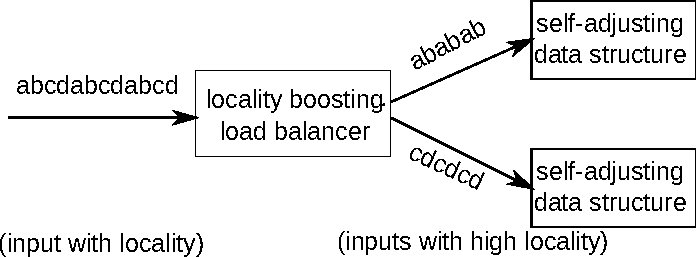
\includegraphics[width=.85\linewidth]{fig/schema.pdf}
  \caption{A locality boosting load balancer partitions the input sequence of a given locality into subsequences with higher locality. Self-adjusting data structures perform better on inputs with higher locality.}
  \label{fig:locality-boosting-lb}
\end{figure}

We distinguish two types of locality in this context. \emph{Spatial locality} means that the distribution of requested items on the entire input domain is statistically biased towards a particular subset of the items. One way to ensure this in the load balancer is to \emph{partition} the input domain into disjunct subsets, so that worker's input distributions are concentrated on a smaller set of inputs. For instance, the hash-based load balancer we used previously to show superlinear scaling with distributed caching is such a partitioning load balancer. In contrast, a round robin or a uniform random load balancer will export its own spatial input locality unchanged to the workers. A related concept is \emph{temporal locality}, which refers to the reuse of specific items in the input within a relatively small time duration. One way to boost temporal locality is to reorder items within a time window: e.g., Reframer applies controlled delays to particular packets in a packet batch to boost temporal locality and, thereby, enable more efficient processing \cite{276946,246322}.

\subsection{Self-adjusting algorithms}
\label{sec:sa-alg}

The second critical enabler for superlinear scaling in our architecture is \emph{self-adjusting algorithms}. Self-adjustment is a general term referring to the property of a dynamic data structure to \emph{automatically reorganize itself based on the sequence of operations it receives}, in order to optimize performance for future operations on frequently accessed or manipulated elements. Internal data reorganization always introduces extra complexity and overhead compared to a static data structure. Therefore, self adjustment can improve performance only if the input processed by the algorithm exhibits a certain amount of spatial or temporal locality.

Next we review the most prominent self-adjusting data structures (but see also \cite{BoseDL08, Avin0020, ParkM12}).

% For further examples, see self-adjusting skip lists~\cite{BoseDL08}, push-down trees~\cite{Avin0020}, or geometric data storages \cite{ParkM12}.

\noindent%
\textbf{Caches.} %
As the simplest but most universal self-adjusting data structure, caches can serve frequently accessed items fast by storing them in a  software or a hardware fast memory. This is typically much faster than if we had to run the request through the full processing pipeline or the slow backing store. Thus, caches have that almost magical capability of self-adaptation, without us having to engineer any prior knowledge of the input into the cache mechanism apart from a promise that it has nontrivial locality. When the promise is true, caches are an inexpensive way to improve throughput and response time. When there is no locality in the input, however, caches usually just add extra latency and overhead.
%
Note that caches do not necessarily have to come in the form of hardware memory: a fast key-value store is a candidate cache for a slow database \cite{10.5555/1012889.1012894}, a kernel fast-path flow cache is a useful way to speed up a slow user-space software switch \cite{188960}, etc.

% However, caches also come with additional complexity and overhead: cache entries have to be created for storing recently accessed data, invalidated when the backing data changes, evicted when the cache is full, and synchronized to consistently represent data that may be present in multiple caches. % Hardware implementations are appealing from this aspect by hiding the extra complexity behind a fast on-chip implementation.

% The performance of a cache is determined by the cache hit rate $\delta$, defined as the ratio of operations served from fast memory to those served on the slow path, and $\rho$, the penalty of a cache miss. In general, for a common LFU or LRU cache the higher the locality in the input and the bigger the cache compared to the input domain, the higher the cache hit rate and the lower the response time. When there is no locality in the input, caches usually just add extra latency and overhead.

\noindent%
\textbf{List lookup.} %
One of the most widely used self-adjusting data structures is the \emph{move-to-front list}. Suppose we wish to store a list of $m$ items in a way so that reordering, insertion and deletion are fast, while lookup is also reasonably efficient. A straightforward choice is a static (singly) linked list. Here, the cost of accessing an item at position $i$ is exactly $i$. Then, any linked list can easily be upgraded to a self-adjusting list using the move-to-front (MTF) heuristics: after accessing an item it is moved to the front, which improves lookup time for future requests of the same item at minimal cost (see Fig.~\ref{fig:mtf-example}). The MTF heuristics comes with appealing theoretical properties, namely that unconditionally moving the accessed item to the front of the list is close to the best one could achieve, even if one knew all future requests \cite{SleatorT85}. MTF can handle both spatial and temporal locality. However, for uniformly distributed input MTF lists usually add nontrivial overhead compared to static lists due to the frequent and useless relinking of the list.

\begin{figure}
  \centering
  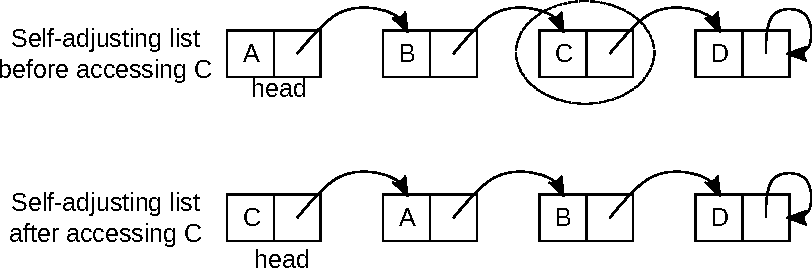
\includegraphics[width=.85\linewidth]{fig/mtf.pdf}
  \caption{A self-adjusting list containing nodes A,B,C and D serves the request to C and moves C to the front of the list to speed up future accesses to C.}
  \label{fig:mtf-example}
\end{figure}

Classic applications of MTF lists are information retrieval systems, compression~\cite{BentleySTW86}, etc. In general, any use case is a potential candidate application for MTF where the task is to match a request against a list of complex rules that do not lend themselves readily to be arranged into a fast lookup structure (e.g., a search tree), like inference in explainable rule-based AI and expert systems \cite{dovsilovic2018explainable}, rule matching in OpenFlow and P4 reference software switches \cite{openflow}, packet classification in networking (see later), etc.  We note that caching is a subset of list lookup, in that every algorithm for list reorganization gives rise to a different cache management algorithm \cite{SleatorT85}.  

\noindent%
\textbf{Search trees.} %
A search tree is an efficient tree data structure for locating specific keys from within an ordered set. A \emph{splay tree} is a self-adjusting version of a static search tree, in that it can dynamically reorganize itself by moving popular items closer to the root of tree and less frequently accessed elements to the bottom, while keeping the tree relatively well-balanced \cite{SleatorT85Splay, BoseDL08, Avin0020}. Since access time in a search tree is determined by the depth at which the requested item is to be found, splay trees can improve future access to the same or similar items when the input exhibits temporal or spatial locality (see Fig.~\ref{fig:bst_root_3}).  Note that a red-black tree, an AVL tree or any similar self-balancing tree is only partially ``self-adjusting'', in that it can rearrange only with respect to the items \emph{stored} in it but not with respect to the queries \emph{posed} to it.

\begin{figure}
 \centering
 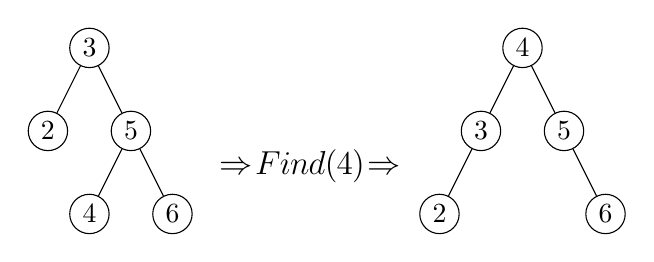
\begin{tikzpicture}[level distance=30pt,
   level 1/.style={sibling distance=30pt},
   level 2/.style={sibling distance=30pt},
   level 3/.style={sibling distance=30pt}]
   % Left
   \node[circle,draw,minimum size=0.5cm,inner sep=1pt] (3a) {3}
   child {node[circle,draw,minimum size=0.5cm,inner sep=1pt] (2a) {2}}
   child {node[circle,draw,minimum size=0.5cm,inner sep=1pt] (5a) {5}
     child {node[circle,draw,minimum size=0.5cm,inner sep=1pt] (4a) {4}}
     child {node[circle,draw,minimum size=0.5cm,inner sep=1pt] (6a) {6}}
   };
   % Right
   \node[circle,draw, minimum size=0.5cm, inner sep=1pt] (4b) at (5.5,0) {4}
   child {node[circle,draw,minimum size=0.5cm,inner sep=1pt] (3b) {3}
     child {node[circle,draw,minimum size=0.5cm,inner sep=1pt] (2b) {2}}
     child[missing] {}
   }
   child {node[circle,draw,minimum size=0.5cm,inner sep=1pt] (5b) {5}
     child[missing] {}
     child {node[circle,draw,minimum size=0.5cm,inner sep=1pt] (6b) {6}}
   };
   % Arrow
   \node (draw=none) at (2.8,-1.5) [font=\large]{$\Rightarrow{Find(4)}\Rightarrow$};
 \end{tikzpicture}
 \caption{Splay-tree with elements 2, 3, 4, 5, 6. After accessing node 4 it is moved to the root that makes a subsequent lookup to it faster, while the tree is kept almost perfectly balanced.}
 \label{fig:bst_root_3}
\end{figure}

\begin{figure*}[t]
  % \begin{tabularx}{\textwidth}{D *{2}{s}}
  \begin{tabular}{m{.3\textwidth} m{.3\textwidth} m{.3\textwidth}}
  % \begin{tabular}{ccc}
    \hspace{28pt}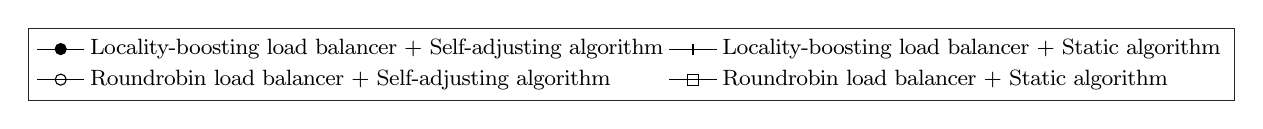
\begin{tikzpicture} 
  \begin{axis}[%
    height=45pt,
    hide axis,
    xmin=10,
    xmax=50,
    ymin=0,
    ymax=0.4,
    legend style={
      draw=white!15!black,
      legend cell align=left,
      legend columns=2,
      font=\footnotesize}
    ]
    \addlegendimage{black,mark=*}
    \addlegendentry{Locality-boosting load balancer + Self-adjusting algorithm}
    \addlegendimage{black,mark=+}
    \addlegendentry{Locality-boosting load balancer + Static algorithm}
    \addlegendimage{black,mark=o}
    \addlegendentry{Roundrobin load balancer + Self-adjusting algorithm}
    \addlegendimage{black,mark=square}
    \addlegendentry{Roundrobin load balancer + Static algorithm}
  \end{axis}
\end{tikzpicture}

%%% Local Variables:
%%% mode: latex
%%% TeX-master: "../distributed_mrf"
%%% End:
\\
    \multirow{-6.4}{*}{\subcaptionbox{List lookup/uniform input\label{fig:multicore-list-uniform}}{\begin{small}
  \begin{tikzpicture}
    \begin{axis}[
      width=165pt,
      height=322pt,
      xlabel={number of CPU cores},
      x label style={at={(0.5,0.01)}},      
      ylabel={Speedup},
      y label style={at={(0.05,0.5)}},      
      xmin=1,
      xmax=48,
      xtick={1,12,24,36,48},
      ymin=0,
      ymax=3300,
      legend style = {
        anchor = north west,
        at = {(0.01, 1.01)},
        font=\tiny,
        % draw = none,
      },
      % scaled y ticks=false
      % no markers
      ]
      % use TeX as calculator:
      \addplot[black,mark=*] table[x=thread,y=speedup,] {fig/list/uniform-100k/multicore_mtf_modulo_uniform.txt};
      % \addlegendentry{Move-to-front/Local LB}
      \addplot[black,mark=+] table[x=thread,y=speedup,each nth point={3}] {fig/list/uniform-100k/multicore_linkedlist_modulo_uniform.txt};
      % \addlegendentry{Linked-list/Local LB}
      \addplot[black,mark=o] table[x=thread,y=speedup,each nth point={3}] {fig/list/uniform-100k/multicore_mtf_roundrobin_uniform.txt};
      % \addlegendentry{Move-to-front/Non-local LB}
      \addplot[black,mark=square] table[x=thread,y=speedup,each nth point={3}] {fig/list/uniform-100k/multicore_linkedlist_roundrobin_uniform.txt};
      % \addlegendentry{Linked-list/Non-local LB}
    \end{axis}
  \end{tikzpicture}
\end{small}

%%% Local Variables:
%%% mode: latex
%%% TeX-master: "../../../distributed_mrf"
%%% End:
}}%
    & \hspace{8pt}\subcaptionbox{List lookup/Zipf input\label{fig:multicore-list-zipf}}{\begin{small}
  \begin{tikzpicture}
    \begin{axis}[
      width=165pt,
      height=322pt,
      xlabel={number of CPU cores},
      x label style={at={(0.5,0.01)}},      
      ylabel={Speedup},
      y label style={at={(0.05,0.5)}},      
      xmin=1,
      xmax=48,
      xtick={1,12,24,36,48},
      ymin=0,
      ymax=3300,
      legend style = {
        anchor = north west,
        at = {(0.01, 1.01)},
        font=\tiny,
        % draw = none,
      },
      % scaled y ticks=false
      % no markers
      ]
      % use TeX as calculator:
      \addplot[black,mark=*] table[x=thread,y=speedup,] {fig/list/uniform-100k/multicore_mtf_modulo_uniform.txt};
      % \addlegendentry{Move-to-front/Local LB}
      \addplot[black,mark=+] table[x=thread,y=speedup,each nth point={3}] {fig/list/uniform-100k/multicore_linkedlist_modulo_uniform.txt};
      % \addlegendentry{Linked-list/Local LB}
      \addplot[black,mark=o] table[x=thread,y=speedup,each nth point={3}] {fig/list/uniform-100k/multicore_mtf_roundrobin_uniform.txt};
      % \addlegendentry{Move-to-front/Non-local LB}
      \addplot[black,mark=square] table[x=thread,y=speedup,each nth point={3}] {fig/list/uniform-100k/multicore_linkedlist_roundrobin_uniform.txt};
      % \addlegendentry{Linked-list/Non-local LB}
    \end{axis}
  \end{tikzpicture}
\end{small}

%%% Local Variables:
%%% mode: latex
%%% TeX-master: "../../../distributed_mrf"
%%% End:
}
    & \subcaptionbox{List lookup/uniform/single-core\label{fig:singlecore-list-uniform}}{\begin{small}
  \begin{tikzpicture}
    \begin{axis}[
      width=250pt,
      height=170pt,
      xlabel={\#thread},
      ylabel={Goodput [million req/sec]},
      xlabel near ticks,
      ylabel near ticks,
      xmin=1,
      xmax=26,
      ymin=0,
      % ymax=10,
      legend style = {
        anchor = north west,
        at = {(0.01, 1.01)},
        font=\scriptsize,
        % draw = none,
      },
      % no markers
      ]
      \addplot[black,mark=*] table[
      x=thread,
      y expr=\thisrowno{4}/1000000
      ]{fig/list/uniform-10/singlecore_mtf_modulo_uniform.txt};
      \addlegendentry{MTF w/ hash-based lb}
      \addplot[black,mark=+] table[
      x=thread,
      y expr=\thisrowno{4}/1000000
      ]{fig/list/uniform-10/singlecore_linkedlist_modulo_uniform.txt};
      \addlegendentry{Static list w/ hash-based lb}
      \addplot[black,mark=o] table[
      x=thread,
      y expr=\thisrowno{4}/1000000
      ]{fig/list/uniform-10/singlecore_mtf_roundrobin_uniform.txt};
      \addlegendentry{MTF w/ round robin lb}
      \addplot[black,mark=square] table[
      x=thread,
      y expr=\thisrowno{4}/1000000
      ]{fig/list/uniform-10/singlecore_linkedlist_roundrobin_uniform.txt};
      \addlegendentry{Static list w/ round robin lb}
    \end{axis}
  \end{tikzpicture}
\end{small}

%%% Local Variables:
%%% mode: latex
%%% TeX-master: "../../../hotnets22"
%%% End:
}
    \\
    & \hspace{8pt}\subcaptionbox{Cache lookup/uniform input\label{fig:multicore-cache-uniform}}{\pgfplotsset{
  RatePlot/.style = {
    tick pos = left,
    xtick align=outside,
    ytick align=outside,
    xlabel near ticks,
    ylabel near ticks,
    width=.4\textwidth,
    height=.3\textwidth,
    legend pos = north west,
    legend cell align=left,
    ylabel = {Throughput [Mpps]},
    xlabel = {number of CPU cores},
    xmin=1, xmax=32,
    ymin=0,
  },
  SpeedupPlot/.style = {
    RatePlot,
    ylabel={Speedup},
  },
  ClassBenchGroupPlot/.style = {
    group/group size = 1 by 2,
    group/horizontal sep = 0pt,
    group/vertical sep = 28pt,
  },
  ClassBenchRatePlot/.style = {
    RatePlot
  },
  ClassBenchSpeedupPlot/.style = {
    SpeedupPlot,
  }
}

%%% Local Variables:
%%% mode: latex
%%% TeX-master: "../distributed_mrf.tex"
%%% End:

%
\begin{small}
  % \tikzmath
  % {
  %   function est(\x)
  %   {
  %     if (\x < 10) then
  %     {
  %       return 0.1+0.9*(0.1*\x +(1-0.1*\x)*10)/\x;
  %     } else {
  %       return 0.1 + 0.9//\x;
  %     };
  %   };
  %   \a = est(4);
  %   \b = est(14);
  % }
  \begin{tikzpicture}
    \begin{axis}[
      width=165pt,
      height=120pt,
      xlabel={\#CPU cores},
      x label style={at={(0.5,0.04)}},
      ylabel={Speedup},
      % xlabel near ticks,
      % ylabel near ticks,
      y label style={at={(0.1,0.5)}},
      xmin=1,
      xmax=35,
      ymin=0,
      xtick={1,10,20, 30},
      % ymax=10,
      legend style = {
        anchor = north west,
        at = {(0.01, 1.01)},
        font=\scriptsize,
        % draw = none,
      },
      % no markers
      ]
      \addplot[SelfAdjustingSimMark,mark size=2pt] table[x=thread,y=speedup,each nth point={3}]{fig/cache/uniform-50k-2/mcore_cache_modulo_uniform.txt};
      % \addlegendentry{Local LB}
      \addplot[SelfAdjustingSimMark,mark=pentagon*,mark size=3pt,each nth point={3}] table[x=thread,y=speedup,each nth point={2}]{fig/cache/uniform-50k-2/mcore_cache_roundrobin_uniform.txt};
      % \addlegendentry{Non-local LB}
      % \addplot[domain=1:25,black,dashed]{x};
      % \addlegendentry{Linear scaling}
      % \addplot[domain=1:25,black,densely dotted]{1/(0.03+0.97/x)};
      % \addlegendentry{Amdahl's law}
      % \addplot[domain=0:25,black,densely dotted]{est(1.0)/est(x)};
      % \node at (100,100) {\a\b};
      % \addlegendentry{T}
      % \addplot[black,mark=o] table[x=thread,y=rate] {fig/cache/uniform-50k/multicore_cache_roundrobin_uniform.txt};
      % \addlegendentry{Round robin lb}
      % \addplot[black,mark=square] table[x=thread,y=rate] {fig/cache/uniform-50k/multicore_scache_roundrobin_uniform.txt};
      % \addlegendentry{staticcache / roundrobin}
    \end{axis}
  \end{tikzpicture}
\end{small}

%%% Local Variables:
%%% mode: latex
%%% TeX-master: "../../../distributed_mrf"
%%% End:
}
    & \subcaptionbox{Tree lookup/uniform input\label{fig:singlecore-tree-uniform}}{\pgfplotsset{
  RatePlot/.style = {
    tick pos = left,
    xtick align=outside,
    ytick align=outside,
    xlabel near ticks,
    ylabel near ticks,
    width=.4\textwidth,
    height=.3\textwidth,
    legend pos = north west,
    legend cell align=left,
    ylabel = {Throughput [Mpps]},
    xlabel = {number of CPU cores},
    xmin=1, xmax=32,
    ymin=0,
  },
  SpeedupPlot/.style = {
    RatePlot,
    ylabel={Speedup},
  },
  ClassBenchGroupPlot/.style = {
    group/group size = 1 by 2,
    group/horizontal sep = 0pt,
    group/vertical sep = 28pt,
  },
  ClassBenchRatePlot/.style = {
    RatePlot
  },
  ClassBenchSpeedupPlot/.style = {
    SpeedupPlot,
  }
}

%%% Local Variables:
%%% mode: latex
%%% TeX-master: "../distributed_mrf.tex"
%%% End:

%
\begin{small}
  \begin{tikzpicture}
    \begin{axis}[
      width=165pt,
      height=120pt,
      xlabel={\#CPU cores},
      x label style={at={(0.5,0.04)}},
      ylabel={Speedup},
      y label style={at={(0.1,0.5)}},
      xmin=1,
      xmax=36,
      xtick={1,10,20,30},
      ymin=0,
      % ymax=370,
      grid=major,
      tick pos = left,
      legend style = {
        anchor = north west,
        at = {(0.01, 1.01)},
        font=\scriptsize,
        % draw = none,
      },
      % scaled y ticks=false
      % no markers
      ]
      % use TeX as calculator:
      \addplot[SelfAdjustingSimMark,mark size=2pt] table[x=thread,y=speedup,each nth point={3}] {fig/tree/uniform-500/multicore_wsplay_modulo_uniform.txt};
      % \addlegendentry{Splay-tree/Local LB}
      \addplot[StaticSimMark,mark size=3pt] table[x=thread,y=speedup,each nth point={3}] {fig/tree/uniform-500/multicore_wbtree_modulo_uniform.txt};
      % \addlegendentry{B-tree/Local LB}
      \addplot[SelfAdjustingSimMark,mark=pentagon*,mark size=3pt] table[x=thread,y=speedup,each nth point={3}] {fig/tree/uniform-500/multicore_wsplay_roundrobin_uniform.txt};
      % \addlegendentry{Splay-tree/Non-local LB}
      \addplot[StaticSimMark,mark=square,mark size=3pt] table[x=thread,y=speedup,each nth point={3}] {fig/tree/uniform-500/multicore_wbtree_roundrobin_uniform.txt};
      % \addlegendentry{B-tree/Non-local LB}
    \end{axis}
  \end{tikzpicture}
\end{small}

%%% Local Variables:
%%% mode: latex
%%% TeX-master: "../../../distributed_mrf"
%%% End:
}
  % \end{tabularx}
  \end{tabular}
  \caption{Static vs. self-adjusting distributed systems scaling laws with round-robin and hash-based load balancing: (a) static vs. MTF list access speedup on uniform input ($m$=100k); (b) static vs. MTF list speedup on skewed input ($m$=100k, Zipf power law with $\alpha=1.01$), (c) static vs. MTF list access goodput with multiple threads running on a \emph{single core} for uniform input ($m$=10k); (d) cache access on uniform input ($m$=50k, $\delta=0.05$, $\rho=100k$ cycles); and (e) static balanced vs. splay tree speedup ($m=500$, $w=100k$ cycles).  Panels (a), (b), (d) and (e) show multicore speedup as the function of the number of CPU cores, each running a single worker, while (c) shows the single-core throughput (goodput) using an increasing number of lightweight parallel threads.}
  \label{fig:dist-self-adjusting-eval}
\end{figure*}

Splay trees are widely used to adaptively speed up associative memory and data compression algorithms \cite{jones1988application}, as well as a building block for more complex self-adjusting algorithms.

% Self-adjusting data structures are widely used in algorithms and computer systems, e.g., in computing point maxima and convex hulls~\cite{BentleyCL93}, organizing lists of identifiers in program compilation and interpretation~\cite{HesterH85}, detecting collisions in hash tables~\cite{HesterH85}, or compressing arbitrary input~\cite{BentleySTW86}. And indeed, every cache management scheme can be viewed as a self-adjusting data structure as well

\subsection{Superlinear scaling}
\label{sec:arch-scaling}

So how can locality-boosting load balancing and self-adjusting algorithms, when used together in a distributed system, produce superlinear scaling? Below we present an example, \emph{distributed self-adjusting list lookup}, along with a performance analysis as demonstration. Our architecture consists of a locality-boosting partitioning load-balancer (see Fig.~\ref{fig:locality-boosting-lb}) combined with a self-adjusting move-to-front list (see Fig.~\ref{fig:mtf-example}) implemented in the workers. The rationale for why this design achieves superlinear scaling is the following.

Suppose that there are $m$ items to be stored in the list and $k$ workers, each maintaining an independent index into the list. Suppose further that, at the input, requests can be received for any of the $m$ items. To make things more difficult we assume uniform request distribution on the system's input, which is, recall, the worst case for any self-adjusting algorithm by being totally \emph{unpredictable}. Thus, for a single worker move-to-front reordering has no useful effect and the worst case access time is $m$, identical to that of a static linked list.

Now suppose we move from 1 worker to $k$ parallel workers. This results that, within our architecture, the load balancer effectively partitions the uniformly distributed input on $m$ items into $k$ uniformly distributed input streams for only $\frac{m}{k}$ different items (see Fig.~\ref{fig:locality-boosting-lb}). This means that the workers' input features a much higher spatial locality than the system's input (which sports none).  Had we used a random or a round robin load balancer the workers would still see all the $m$ possible inputs, just with a sampled uniform distribution, and no locality. After a while, each MTF list in the workers will have its specific subset of $\frac{m}{k}$ items moved to the first $\frac{m}{k}$ positions (in an arbitrary order), reducing the worst-case lookup time from $m$ (1 worker) to $\frac{m}{k}$ ($k$ workers). This introduces $k\times$ speedup compared to the single-threaded case.

Then, superlinear speedup is merely a product of two simultaneous $k\times$ speedup factors: one $k\times$ speedup comes from the self-adjusting list getting progressively faster as we add new workers (recall the ``scaled size'' model from \S\ref{sec:backgound-dist-cache}), and another $k\times$ speedup because we extend the total compute capacity available to the system $k$ times. The effective speedup is then just the multiple of the two, yielding $k^2$ times speedup in total. Plugging into Amdahl's law we get the \emph{scaling law for distributed MTF lists} (see the scaling law in Fig.~\ref{fig:amdahl}):
\begin{equation}\label{eq:mtf-perf}
  S_l(k) = \frac{T_l(1)}{T_l(k)} = \frac1{s + \frac{1-s}{k^2}} \enspace .
\end{equation}

% We used this scaling law as the graphical illustration for superlinear scaling in Fig.~\ref{fig:amdahl}. 
For small values of $k$ we obtain $O(k^2)$ scaling, despite that uniform request distribution is the worst case for self-adjustments. This hints at a great future potential for networking workloads that typically exhibit highly skewed request distributions~\cite{832484}.

\subsection{Evaluation}
\label{sec:sims}

Fig.~\ref{fig:dist-self-adjusting-eval} presents the results from a comprehensive simulation study we conducted to understand distributed self-adjusting systems performance over a broad selection of load balancing policies, self-adjusting algorithms, and input distributions. The simulator was coded in roughly 1,000 lines of Go and uses lightweight threads (goroutines) managed by the Go runtime to run a given number of workers in parallel. We used a simple home-grown implementation for static and MTF lists and standard Go modules for LRU caches \cite{golang-lru}, static balanced trees \cite{golang-btree} and splay trees \cite{golang-splay}. In order to make tree lookup CPU bounded we used an ``expensive'' order underneath the tree, where every comparison operation costs a configurable $w$ number of extra cycles. The simulator creates the specified combination of a load balancer, $k$ worker threads running the selected lookup algorithm, and a random input sequence with a given request distribution, and then performs a configurable number of lookup operations and measures the total execution time with nanosecond precision. To obtain a full picture, the total execution time includes the transient time needed to warm up the self-adjusting algorithms running in the threads. For the specification of the evaluation platform, refer to \S\ref{sec:sa-nf-tables-eval}.

Our observations are as follows. First, it is immediate that \emph{the right combination of a locality boosting load balancer and a self-adjusting algorithm robustly delivers superlinear speedup}, irrespectively of the problem domain or the input distribution. Even for a worst-case uniform request distribution, we obtain $3,300\times$ speedup(!) for list access on 48 CPU cores, almost $70\times$ of ``ideal'' linear speedup, $200\times$ speedup on LRU caches and $65\times$ speedup on tree search with 36 CPU cores. Usually the superlinear growth is so dominant that we can hardly put the Amdahl's scaling on the same diagram.  Second, \emph{only the combination of locality-boosting load balancing and self-adjusting algorithms produces superlinear speedup}, all other combinations (i.e., round robin with any algorithm or static algorithm with any load balancer) fall back to Amdahl's scaling.  Third, \emph{self-adjustment clearly has its overhead}. This can be observed in Fig.~\ref{fig:singlecore-list-uniform}, which, instead of the relative speedup shows the absolute throughput. Here, the single-threaded self-adjusting version is clearly slower than the static version (a trait we identified in essentially all cases with uniform input). Fourth, \emph{the overhead of self-adjustment becomes irrelevant for more than one CPU core, or with skewed request distributions}. For instance on a Zipf input distribution (Fig.~\ref{fig:multicore-list-zipf}) even the single-threaded self-adjusting version is already $2$--$2.5\times$ faster in an absolute term irrespectively of the load balancer (not shown in the figure). However, \emph{only} combining with a locality-boosting load balancer it produces superlinear speedup.

And finally a rather surprising finding. In Fig.~\ref{fig:singlecore-list-uniform} we show an evaluation that was executed with an increasing number of parallel threads manually constrained to run with at most 110\% CPU utilization using \texttt{cpulimit}. This effectively simulates a single core worth of total CPU shared by \emph{all} the parallel workers, with a little surplus for the load balancer. The results indicate that the distributed self-adjusting system (but \emph{only} this combination!) delivers linear speedup with adding new threads. With uniformly distributed requests, we achieve $25\times$ speedup by spawning 25 parallel goroutines, each sharing a single CPU core.  And this is despite that the overhead of request generation, goroutine scheduling, and memory management all count towards the total system load and take away precious CPU time from the useful workload.

But how can parallelization benefit performance when we do not even add more CPU power to the system? Recall, in the multicore case superlinear speedup emerges thanks to the superposition of two independent $k\times$ speedup trends, one delivered by the self-adjusting workers and another added by us throwing $k\times$ more CPU power to the system. When the total available CPU is limited only first $k\times$ speedup factor is in effect, resulting in the observed linear scaling trend.

% glitches are cpu architecture specific

% LET's SKIP THIS: highly speculative!!!!!!!!!!!1
%
% \subsection{Revised Amdah's law}
% \label{sec:sims}

% An interpretation of superlinear scaling: if we introduce the notion of the ``virtual job size''. Implicit in Amdahl's law \eqref{eq:amdahl} is that the job size remains the same independently of $k$. Parallel self-adjustments, however, may actually \emph{decrease} the amount of work each worker has to perform per each request. Let $b(k)$ denote the ``virtual job size'' perceived by each worker when the number of  workers is $k$. We observe that in parallel self-adjusting systems $b(k)$ is decreasing in $k$; e.g., for MTF we have $b(k) = \frac1{k}$.

% \begin{equation}\label{eq:revised-amdahl}
% S(k) = \frac{T(1)}{T(k)} = \frac{1}{s + \frac{1-s}{k^{\alpha}}} \enspace .
% \end{equation}

% Amdah's law for $\alpha=1$, distributed MTF scaling for $\alpha=1$, superlinear scaling with $\alpha>1$

%%% Local Variables:
%%% mode: latex
%%% TeX-master: "distributed_mrf"
%%% End:



% !TEX ROOT = ./distributed_mrf.tex
\section{Superlinear scaling in distributed caching}\label{sec:dist-caching}

The most prominent example for the scaled size model is \emph{distributed caching} \cite{scalability-analyzed, sdn-analytitcs, dobb-2} (for complete taxonomies see \cite{556383, 7733347, 80148}).  Most modern CPUs come with unshared Level-1 fast cache memory: the more CPU cores, the more fast memory is available for caching, which improves the cache-hit rate at the workers. This tends to speed up memory\slash cache-bound code disproportionately. Many distributed applications also contain a fast-path\slash cache; e.g., \texttt{memcached} is often used as a fast cache for a ``slow'' web service \cite{180324,10.5555/1012889.1012894}, popular keys are cached in the OS kernel for fast key-value store access \cite{179747, ghigoff2021bmc}, FIB caches maintain the most recent IP routes to sidestep longest prefix matching \cite{rottenstreich2016optimal}, hierarchical flow caches serve as a fast-path in programmable software switches \cite{188960}, etc. All these workloads may benefit from the caches becoming more efficient as the system is scaled and, potentially, show superlinear speedup on certain workloads. % We stress, however, that faster-than-linear speedup is strictly contingent on the way work is distributed across workers so that subproblem sizes indeed reduce, otherwise cache efficiency remains constant and superlinear growth vanishes (see later).

\begin{figure}
  \centering
  \begin{small}
    \begin{small}
  \tikzmath
  {
    function lookup(\x)
    {
      if (\x < 10) then
      {
        return 0.1+0.9*(0.1*\x +(1-0.1*\x)*10)/\x;
      } else {
        return 0.1 + 0.9/\x;
      };
    };
    function dcache(\x)
    {
      return lookup(1.0)/lookup(\x);
    };
    function rrcache(\x)
    {
      return lookup(1.0)/(0.1+0.9*(0.1 +(1-0.1)*10)/\x);
    };
    function pcache(\x)
    {
      return lookup(1.0)/(0.1+0.9/\x);
    };
    \a = dcache(1);
    \b = lookup(1.0);
  }
  \begin{tikzpicture}
    \begin{axis}[
      width=250pt,
      height=170pt,
      xlabel={\#threads},
      ylabel={Speedup},
      xlabel near ticks,
      ylabel near ticks,
      xmin=0,
      xmax=20,
      ymin=0,
      ymax=67,
      xtick={1,5,10,15,20},
      legend style = {
        anchor = north west,
        at = {(0.01, 1.01)},
        font=\scriptsize,
        % draw = none,
      },
      % no markers
      ]
      \addplot[domain=0:25,black,solid]{dcache(x)};
      \addlegendentry{Hash-based load balancing}
      \addplot[domain=0:25,black,densely dotted]{rrcache(x)};
      \addlegendentry{Random load balancing}
      \addplot[domain=0:25,black,densely dashed]{pcache(x)};
      \addlegendentry{All requests hit the cache}
      % \node at (25,25) {\a, \b};
    \end{axis}
  \end{tikzpicture}
\end{small}

%%% Local Variables:
%%% mode: latex
%%% TeX-master: "../distributed_mrf"
%%% End:

\end{small}
\caption{Scaling laws for distributed caching: hash-based load balancing, lower envelope (round robin load balancing) and upper envelope (perfect cache hit rate with $k$ caches). }
  \label{fig:dcache-analysis}
\end{figure}

% refer to "Modeling Speedup (n) Greater than n" -> analysis

% assumption for the analysis? ``I think equation 2 should be explained much better. It is not at all obvious (not sure even correct) that hit rate scales linearly with threads (I think only true is delta << 1). What is $\rho$ exactly the ratio of (fetching time in the event of miss) / (fetching time in the event of a catch hit)?''

It is instructive to quantify superlinear speedup in this context using a simple model. Suppose a source emits uniformly distributed random requests for $m$ items and requests are distributed among $k$ workers, each using a separate cache of size $c$, by hashing on the request id.  Initially, the cache hit rate for a single worker that processes all $m$ possible requests is $\delta := \sfrac{c}{m}$. Adding $k$ workers effectively partitions the requests into $k$ random buckets so that each worker will perceive uniformly distributed requests for only $\sfrac{m}{k}$ items, which improves the cache hit rate at each worker to $\frac{c}{\sfrac{m}{k}} = k\delta$ ($k\delta \le 1$). This puts the lookup time of the system of $k$ parallel caches to
\begin{align}\label{eq:dist-cache}
  T_c(k) = \begin{cases} s + \frac{1-s}{k}(k\delta + (1-k\delta)\rho) & \text{if } k\delta \le 1\\s + \frac{(1-s)}{k} & \text{otherwise}\end{cases} \enspace ,
\end{align}
where $\rho$ is the penalty for a cache miss event, $\delta$ is the cache hit rate for a single worker, and $s$ denotes the fraction of execution time spent in the sequential part of the code.


The speedup $S_c(k)=\frac{T_c(1)}{T_c(k)}$ for the parameters $s=0.1$, $\delta=0.1$ and $\rho=10$ is depicted in Fig.\ref{fig:dcache-analysis}. The lower envelope of the scaling profile is given by Amdahl's law for the system with random or round robin load-balancing. % ($\frac{T_c(1)}{s + \frac{1-s}{k}(\delta + (1-\delta)\rho)}$).
As $k$ grows the scaling profile progresses over a superlinear curve to an elevated Amdahl's law profile, representative of a system serving \emph{all} requests from fast memory. % ($\frac{T_c(1)}{s + \frac{1-s}{k}}$).
Note that this occurs \emph{only} if request dispatching is chosen carefully to partition the item space. Modulo hashing assigns the same item to the same worker deterministically, so that workers process only a subset of the items that may have a greater chance to fit into the cache. In contrast, a random or a round robin load balancer may assign any item to any worker, which defeats the purpose of improving workers' cache hit rate. % and destroys superlinear scaling all together. % (see empirical evidence in the next Section).

%%% Local Variables:
%%% mode: latex
%%% TeX-master: "distributed_mrf"
%%% End:


% !TEX ROOT = ./distributed_mrf.tex
\section{Case study 2: Superlinear scaling\\ in the Linux kernel}\label{sec:dist-classifier}

We present a case study for systematically applying the distributed self-adjusting systems architecture to a common networking problem: software packet classification \cite{gupta2001algorithms}. The goal is to demonstrate the general engineering methodology by assembling \emph{existing} techniques into a distributed self-adjusting scheme and understand when, and to what extent, superlinear scaling emerges. We consider it a success if we can robustly reproduce faster-than-linear growth on some realistic workloads. It is a stated \emph{nongoal} to conceive novel algorithms, let alone produce the fastest software packet classifier. % (that award undeniably goes to DPDK \texttt{rte\_acl} \cite{rte-acl})
Yet, our self-adjusting firewall implemented in the Linux kernel will prove several times faster than the default Linux kernel implementation on a wide range of workloads.

To achieve superlinear scaling we need a self-adjusting algorithm in the first place (plus a locality-boosting load balancer). From the many potential use cases % for which a self-adjusting algorithm exists
\cite{SleatorT85Splay, BentleyCL93, HesterH85, HesterH85, BentleySTW86, Avin0020, ParkM12} we eventually chose packet classification for the following reasons.  First, the default Linux firewall implementation, \nftables, uses a static doubly linked list to evaluate classifier rules, which makes it an appealing candidate for applying the move-to-front (MTF) heuristics (but see ramifications related to handling rule-dependencies below). % which will buy us the non-self-adjusting baseline for free.
Second, underlying packet classification, there is an infamously difficult theoretical problem \cite{10.1145/2619239.2626294,10.1006/jagm.1996.0063, PacutVAPRS2022, 10.1145/2619239.2626294, 10.1145/1851182.1851208, 10.1145/863955.863980, gupta2001algorithms}, % , 10.1145/3359989.3365431},
and achieving superlinear speedup on such a hard problem promises massive performance gain. Third, the Linux kernel network stack offers several flexible software and hardware based load balancers for dispatching packets to parallel classifier instances running on different CPU cores \cite{rss-linux}, which we will reuse to implement the locality-boosting load balancer component. And fourth, packet classifiers are very difficult to cache \cite{1354643} (recall, caches are the ``cheap'' way to obtain superlinear scaling), which calls for a true self-adjusting packet classifier. % algorithm that goes beyond caching. % \cite{10228937}.

% \subsection{The Linux packet classifier}
% \label{sec:sa-pack-class}

\subsection{Self-adjusting packet classification}
\label{sec:sa-sa-pack-class}

A network firewall is a means to control incoming and outgoing network traffic based on user-defined packet classifier rules (see Fig.~\ref{fig:class-sample}). % This is useful to improve security, control access, filter and protect against ongoing attacks, and log\slash monitor network activity.
A classifier \emph{rule} is a pair of a filter, a user-defined regular expression defined on specific fields of the packet header or metadata, and an action that decides what to do with the packets that match the filter (accept, drop, log, etc.).  Rules are organized into linear chains ordered by rule priority. When a packet enters a chain, it is compared against the first rule. If there is a match, the corresponding action is executed and the lookup is over. Otherwise, subsequent rules are matched in priority order until the first match is found.

% The Linux kernel contains several built-in packet classifiers.
The \nftables kernel engine adds a virtual machine to the Linux kernel that uses a DSL for parsing and matching packet header fields \cite{nftables}. This makes \nftables agnostic to specific network protocols, in contrast to, e.g., \texttt{iptables}, which contains an embedded protocol parser. Currently, \nftables is the default packet classifier in most Linux distributions.

\begin{figure}[t]
  \centering
  \begin{small}
    \renewcommand{\tabcolsep}{2pt}
    \begin{tabular}{r|l|l|r|r|l}
      \textbf{Prio} & \textbf{Proto} & \textbf{Src IP} & \textbf{Dst IP} & \textbf{Dst Port} & \textbf{Action}\\
      \hline
      1 & UDP & 192.168.178.33   & 23.0.0.45  & 53  & ACCEPT\\
      2 & TCP & 10.10.10.0/24    & 23.0.0.45  & 443 & DROP\\
      3 & UDP & 192.168.178.0/24 & 23.0.0.45  & 53  & DROP\\
      4 & TCP & 10.10.10.10/32   & 23.0.0.45  & ANY & ACCEPT\\
      5 & IP  & 192.168.0.0/16   & 23.0.0.0/8 & ANY & ACCEPT\\
    \end{tabular}
  \end{small}%
  \caption{Sample firewall rule set. Source ports do not matter.}
  \label{fig:class-sample}
\end{figure}

One way to make \nftables self-adjusting would be to replace the static linked list it uses internally for rule matching with a self-adjusting list. A naive application of MTF, however, would easily break the semantics of the firewall. This is because rules in the chain may not be independent from each other, and hence may not be freely swapped \cite{10.1145/2619239.2626294}.

Consider the example in Fig.~\ref{fig:class-sample} and suppose that, initially, rules are ordered priority-wise in the list: $\langle1, 2, 3, 4, 5\rangle$. Suppose that a packet with the IP 5-tuple (192.168.0.1, 23.0.0.45, UDP, 1, 3478) enters the classifier, where the fields in the 5-tuple are IP source and destination address, protocol, and source and destination port, respectively. Rules are inspected in linear order until rule 5 is found as the first match, at which point the lookup terminates with the verdict ACCEPT. Now, a naive application of MTF would move rule 5 to the front of list, resulting in the order $\langle5, 1, 2, 3, 4\rangle$. Suppose another packet with the 5-tuple (192.168.178.1, 23.0.0.45, UDP, 1, 53) is to be processed next: this will immediately match rule 5 at the front of the list yielding the verdict ACCEPT, despite that, if matched in priority order, rule 3 would be the correct match and the verdict should be DROP. % To maintain correctness, the furthest we can move rule 5 towards the front of the list is the position immediately after its dependency, rule 3.

We say that rule $u$ is \emph{dependent} on another rule $v$ if they have overlapping match criteria in all fields, $v$ has a higher priority than $u$, and $u$ and $v$ define different actions. Such a dependency means that $u$ is not allowed to be moved before $v$ in the list, otherwise some packets may be erroneously classified. For instance, in the example of Fig.~\ref{fig:class-sample} rule 5 is dependent on rule 3, which is in turn dependent on rule 1, implying the dependency chain $5\to 3\to 1$. Similarly, rule $4$ is dependent on rule $2$. % Rule dependencies define a Directed Acyclic Graph (DAG) in the graph whose nodes are the set of rules, where there is an edge $(u, v)$ from $u$ to $v$ if $u$ is dependent on $v$ (see Fig.~\ref{fig:class-dep}).

% \begin{figure}[t]
%   \centering
%   \begin{small}
%     \begin{tikzpicture}[->,>=stealth,node distance=2.5cm, auto, every node/.style={circle,draw,minimum size=0.5cm,inner sep=2pt}]
%       % Branch 1
%       \node[circle,draw] (5) {5};
%       \node[circle,draw,right of=5] (3) {3};
%       \node[circle,draw,right of=3] (1) {1};

%       % Branch 2
%       \node[circle,draw,below of=5,yshift = 1.5cm] (4) {4};
%       \node[circle,draw,right of=4] (2) {2};

%       % Edges
%       \draw (5) -- (3);
%       \draw (3) -- (1);
%       \draw (4) -- (2);
%     \end{tikzpicture}
%   \end{small}
%   \caption{Dependency graph}%
%   \label{fig:class-dep}
% \end{figure}

A dependency-aware variant of the MTF heuristics, called the \emph{Move-recursively-Forward} (MRF) algorithm, is defined in \cite{10228937} (see Alg.~\ref{alg:mrf}). The idea is to push an accessed item forward in the list until the first dependency is reached. To prevent the item from blocking behind its direct dependency, the dependency is also moved forward until the first transitive dependency is hit. This process repeats until the head of the list is reached.  Independent rules are however free to be moved without restrictions, to the point that if there are no dependencies then MRF simplifies into a plain MTF policy.  Contrarily, if the entire rule set is a single dependency chain then no reordering is allowed and MRF degrades into a static list. In general, MRF moves frequently hit rules, with all their dependencies, to the first positions of the chain, which tends to improve lookup performance on high-locality input without jeopardizing the semantics of the classifier \cite{10228937}. In addition, MRF is ``almost''optimal in the same competitive sense as MTF, in that the best reordering one could obtain even if one knew the entire lookup sequence in advance would yield only a small constant factor improvement over MRF.

\begin{algorithm}[t]
  \caption{Move Recursively Forward (MRF)}
  \label{alg:mrf}
  \begin{small}
    \begin{algorithmic}[1]
      \Procedure{MRF}{$y$}
      \If{$y$ has no dependencies}
      \State Move $y$ to the front of the list
      \Else
      \State Let $z$ be the direct dependency of $y$
      \State Move node $y$ to position$(z) + 1$
      \State \Call{MRF}{$z$}
      \EndIf
      \EndProcedure
    \end{algorithmic}
  \end{small}
\end{algorithm}

Going back to our earlier example, after rule $5$ is hit in the list $\langle1, 2, 3, 4, 5\rangle$ MRF moves it immediately after the direct dependency $3$ along the dependency chain $5\to 3\to 1$, $3$ is moved to the position after $1$, and the recursion ends resulting the order $\langle1, 3, 2, 5, 4\rangle$. If $5$ was hit again, the lookup time would be only $4$ instead of $5$. Then, $5$ would be moved forward again, yielding the order $\langle1, 3, 5, 2, 4\rangle$ and a lookup time of $3$. Note that dependency chains can be moved by MRF independently from each other: e.g., if $4$ was hit first then we would obtain $\langle2, 1, 4, 3, 5\rangle$ in the first iteration and eventually $\langle2, 4, 1, 3, 5\rangle$, with lookup time for $4$ dropping from $4$ to $2$.

We created a comprehensive self-adjusting packet classifier implementation on top of \nftables using the dependency-aware MRF algorithm \cite{10228937}. Our implementation can run multiple MRF instances in parallel, each maintaining its own local rule order in a private per-CPU pointer array that indexes into a shared static rule list. Apart from lockless list reordering, this also enables lockless rule addition\slash deletion: every time the rule list is updated we simply allocate a new pointer array at each CPU and update the list head atomically.

The original MRF algorithm uses recursion (see Alg.~\ref{alg:mrf}), which may be expensive in the Linux kernel due to the overhead of maintaining the function call stack. To avoid this overhead, we defined an iterative version of the algorithm. When a rule is to be moved forward, we first check whether it can be swapped with the preceding rule. This is done by checking whether the two rules overlap using a range-based representation, which we extract from the rule's bytecode in the \nftables virtual machine. If there is an overlap then the rule cannot be moved forward so we restart the process, this time trying to move the blocking dependency forward. Otherwise, the two rules are independent so they are immediately swapped and the iteration moves to the subsequent preceding rule. Reordering terminates when we reach the first position. A more efficient implementation would be to precompute dependencies on rule insertion\slash deletion and run the MRF algorithm using the cached dependencies; implementing this optimization is for further study. %. This, however, would complicate code and make insertions more expensive. % , and may even end up being slower since recursion in the kernel can be costly due to the overhead of a potentially deep call stack.

\subsection{Locality-boosting load balancing for\\ packet classification}
\label{sec:sa-rss}

The other ingredient that we need to achieve faster-than-linear scaling is a locality-boosting load balancer.  An ideal load balancer would partition the rule set into disjoint per-worker subsets. This would minimize the size of the \emph{active rule set} at workers, which is defined as the set of rules for which a particular worker receives packets during a time window. The smaller the active rule set the fewer rules the classifier has to search through for each packet and the larger the contribution of self-adjustment to superlinear speedup. Contrarily, the larger the active rule set the more rules compete for the first positions in the list, which reduces the room for self-adjustment to reduce lookup time and erodes superlinear scaling.

There are several factors that may bloat workers' active rule sets. First, whenever a rule with nonzero dependencies is hit MRF adds its entire dependency chain to the active rule set. Second, packet classifiers often use wildcard rules, matching potentially a huge number of diverse traffic flows. If the load balancer dispatches two packets matching the same rule to two different workers, then both workers would have to include the same rule, with all its dependencies, in its active rule set (see an example in Fig.~\ref{fig:active-set-lb}). Note that the same rule duplication problem plagues many software packet classifier algorithms \cite{10.1145/863955.863980, 820051, 10.1145/1851182.1851208, 8485947}.

Designing an ideal load balancer that minimizes workers' active rule sets, regardless of rule dependencies and flow diversity, seems difficult (but see a discussion in \S\ref{sec:related-work}). Therefore, we adopt a simple hash-based load balancing scheme here that implements only an ``imperfect rule set partitioning''. Our load balancer will however be fully implemented in hardware and run at line rate. This is crucial to minimize the overhead, which in our system entirely counts towards the sequential part of the workload and limits ultimate scaling.  Later, we will show empirically that even this imperfect scheme is enough to reach superlinear speedup in many practical cases.

Our load balancer reuses the Receive Side Scaling (RSS, \cite{10.1145/3359989.3365412, rss-linux}) function offered by most standard NICs. RSS evaluates a hash function over a selected set of header fields per each packet. The resultant hash value is then used to index into an indirection table to select a packet queue, and the corresponding CPU core, that will process the packet. The hash function can be configured to consider any combination of the IP 5-tuple header fields, which allows us to fine-tune locality-boosting in our load balancer.

\begin{figure}[t]
  \centering
  \subfloat[][Imperfect separation]{
    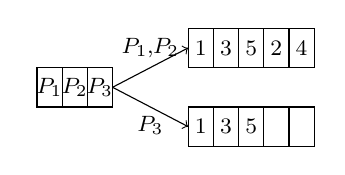
\begin{tikzpicture}[font=\footnotesize]
    % Define the width and height of the rectangles
    \def\rectwidth{0.32}
    \def\rectheight{0.5}
    \def\listdist{1.6}
        
    % Draw the queue
    \draw (-\rectwidth,0) rectangle (\rectwidth,\rectheight);
    \node at (-\rectwidth/2,\rectheight/2) {$P_1$};

    \draw (0,0) rectangle (\rectwidth,\rectheight);
    \node at (\rectwidth/2,\rectheight/2) {$P_2$};

    \draw (\rectwidth,0) rectangle (2*\rectwidth,\rectheight);
    \node at (\rectwidth+\rectwidth/2,\rectheight/2) {$P_3$};
%     
    % Add arrows from the head of the queue
    \draw[->] (2*\rectwidth,\rectheight/2) -- (\listdist,3*\rectheight/2) node[midway, above] {$P_1$,$P_2$};
    \draw[->] (2*\rectwidth,\rectheight/2) -- (\listdist,-\rectheight/2) node[midway, below] {$P_3$};
  
    \foreach \x in {0,1,2,3,4} {
      \draw (\listdist+\x*\rectwidth,\rectheight) rectangle (\listdist+\x*\rectwidth+\rectwidth,2*\rectheight);
      \draw (\listdist+\x*\rectwidth,-\rectheight) rectangle (\listdist+\x*\rectwidth+\rectwidth,0);
    }

    \node at (\listdist+\rectwidth/2,-\rectheight/2) {1};
    \node at (\listdist+\rectwidth+\rectwidth/2,-\rectheight/2) {3};
    \node at (\listdist+2*\rectwidth+\rectwidth/2,-\rectheight/2) {5};

    \node at (\listdist+\rectwidth/2,3*\rectheight/2) {1};
    \node at (\listdist+\rectwidth+\rectwidth/2,3*\rectheight/2) {3};
    \node at (\listdist+2*\rectwidth+\rectwidth/2,3*\rectheight/2) {5};
    \node at (\listdist+3*\rectwidth+\rectwidth/2,3*\rectheight/2) {2};
    \node at (\listdist+4*\rectwidth+\rectwidth/2,3*\rectheight/2) {4};
\end{tikzpicture}

%%% Local Variables:
%%% mode: latex
%%% TeX-master: "../distributed_mrf"
%%% End:

    \label{fig:active-rule-imperfect-lb}
  }
  % \hspace{-1em}
  \subfloat[][Perfect separation]{
    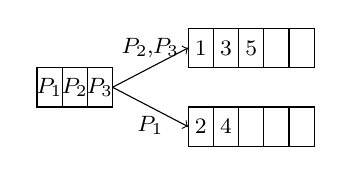
\begin{tikzpicture}[font=\footnotesize]
    % Define the width and height of the rectangles
    \def\rectwidth{0.32}
    \def\rectheight{0.5}
    \def\listdist{1.6}
        
    % Draw the queue
    \draw (-\rectwidth,0) rectangle (\rectwidth,\rectheight);
    \node at (-\rectwidth/2,\rectheight/2) {$P_1$};

    \draw (0,0) rectangle (\rectwidth,\rectheight);
    \node at (\rectwidth/2,\rectheight/2) {$P_2$};

    \draw (\rectwidth,0) rectangle (2*\rectwidth,\rectheight);
    \node at (\rectwidth+\rectwidth/2,\rectheight/2) {$P_3$};
%     
    % Add arrows from the head of the queue
    \draw[->] (2*\rectwidth,\rectheight/2) -- (\listdist,3*\rectheight/2) node[midway, above] {$P_2$,$P_3$};
    \draw[->] (2*\rectwidth,\rectheight/2) -- (\listdist,-\rectheight/2) node[midway, below] {$P_1$};

    \foreach \x in {0,1,2,3,4} {
      \draw (\listdist+\x*\rectwidth,\rectheight) rectangle (\listdist+\x*\rectwidth+\rectwidth,2*\rectheight);
      \draw (\listdist+\x*\rectwidth,-\rectheight) rectangle (\listdist+\x*\rectwidth+\rectwidth,0);
    }

    \node at (\listdist+\rectwidth/2,-\rectheight/2) {2};
    \node at (\listdist+\rectwidth+\rectwidth/2,-\rectheight/2) {4};
    \node at (\listdist+2*\rectwidth+\rectwidth/2,-\rectheight/2) {};

    \node at (\listdist+\rectwidth/2,3*\rectheight/2) {1};
    \node at (\listdist+\rectwidth+\rectwidth/2,3*\rectheight/2) {3};
    \node at (\listdist+2*\rectwidth+\rectwidth/2,3*\rectheight/2) {5};
    \node at (\listdist+3*\rectwidth+\rectwidth/2,3*\rectheight/2) {};
    \node at (\listdist+4*\rectwidth+\rectwidth/2,3*\rectheight/2) {};
\end{tikzpicture}

%%% Local Variables:
%%% mode: latex
%%% TeX-master: "../distributed_mrf"
%%% End:

    \label{fig:active-rule-perfect-lb}
  }
  \caption{Locality-boosting load balancing over packet sequence $P_1$ (matching rule 4 of the sample classifier in Fig.~\ref{fig:class-sample}) followed by $P_2$ and $P_3$ (both matching rule 5): (a) hash-based load balancing may assign $P_2$ and $P_3$ to different workers so that both will have to keep the dependency list $5\to 3\to 1$ in the active rule set, (b) perfect separation sends $P_1$ and $P_2$ to the same worker, yielding minimal active rule sets.}
  \label{fig:active-set-lb}
\end{figure}

% \subsection{Implementation}
% \label{sec:sa-nf-tables-impl}

\subsection{Reproducing superlinear speedup}
\label{sec:sa-nf-tables-eval}

We conducted several experiments with the distributed self-adjusting packet classifier combined with the hash-based RSS load balancer. Our goal was to understand whether superlinear scaling can be robustly reproduced on a real network application using real packet I/O. % Further,  we aim to determine the conditions (rule sets, flow size, etc) under which it emerges.

\begin{figure*}[t]
  \centering

  \resizebox{0.9\textwidth}{!}{%
  \subfloat[][acl1]{
    \pgfplotsset{
  RatePlot/.style = {
    tick pos = left,
    xtick align=outside,
    ytick align=outside,
    xlabel near ticks,
    ylabel near ticks,
    width=.4\textwidth,
    height=.3\textwidth,
    legend pos = north west,
    legend cell align=left,
    ylabel = {Throughput [Mpps]},
    xlabel = {number of CPU cores},
    xmin=1, xmax=32,
    ymin=0,
  },
  SpeedupPlot/.style = {
    RatePlot,
    ylabel={Speedup},
  },
  ClassBenchGroupPlot/.style = {
    group/group size = 1 by 2,
    group/horizontal sep = 0pt,
    group/vertical sep = 28pt,
  },
  ClassBenchRatePlot/.style = {
    RatePlot
  },
  ClassBenchSpeedupPlot/.style = {
    SpeedupPlot,
  }
}

%%% Local Variables:
%%% mode: latex
%%% TeX-master: "../distributed_mrf.tex"
%%% End:


\begin{tikzpicture}

 \begin{groupplot}[ClassBenchGroupPlot]

  \nextgroupplot[ClassBenchSpeedupPlot]

  \addplot coordinates {
     (1, 1.00000)
     (2, 2.01275)
     (3, 2.99326)
     (4, 4.03999)
     (5, 5.02312)
     (6, 6.02253)
     (7, 7.01021)
     (8, 8.04299)
     (9, 9.02064)
     (10, 10.03534)
     (11, 11.10694)
     (12, 12.08788)
     (13, 13.07358)
     (14, 14.01179)
     (15, 15.05161)
     (16, 16.13280)
     (17, 17.14857)
     (18, 18.07133)
     (19, 19.04549)
     (20, 20.20622)
     (21, 21.20803)
     (22, 22.09785)
     (23, 23.04393)
     (24, 24.23765)
     (25, 25.17218)
     (26, 26.28756)
     (27, 27.06453)
     (28, 27.74060)
     (29, 28.61572)
     (30, 29.48150)
     (31, 30.28735)
     (32, 31.37051)
     (33, 31.31105)
     (34, 31.46892)
     (35, 31.41659)
     (36, 31.50497)
     (37, 31.88759)
     (38, 31.98595)
     (39, 32.18120)
     (40, 32.26755)
     (41, 32.51116)
     (42, 32.68041)
     (43, 33.08639)
     (44, 33.06703)
     (45, 33.14436)
     (46, 33.23806)
     (47, 33.46593)
     (48, 33.40066)
     (49, 33.61066)
     (50, 33.73653)
     (51, 34.05734)
     (52, 34.13124)
     (53, 34.31725)
     (54, 34.47786)
     (55, 34.61957)
     (56, 34.64922)
     (57, 34.57655)
     (58, 34.92709)
     (59, 34.83238)
     (60, 35.29259)
     (61, 35.46089)
     (62, 35.39285)
     (63, 35.38630)
    };
    \addlegendentry{Static}

  \addplot coordinates {
     (1, 1.00000)
     (2, 2.78880)
     (3, 5.34148)
     (4, 8.50314)
     (5, 12.18752)
     (6, 16.29228)
     (7, 20.91828)
     (8, 25.42996)
     (9, 30.76640)
     (10, 35.64435)
     (11, 42.18526)
     (12, 47.99208)
     (13, 54.94981)
     (14, 61.30928)
     (15, 67.57976)
     (16, 76.48709)
     (17, 84.80360)
     (18, 88.83299)
     (19, 98.87346)
     (20, 105.97422)
     (21, 117.95420)
     (22, 124.30595)
     (23, 130.33294)
     (24, 141.99362)
     (25, 151.39788)
     (26, 164.00849)
     (27, 169.80391)
     (28, 181.86091)
     (29, 191.72184)
     (30, 196.66672)
     (31, 210.59534)
     (32, 225.16466)
     (33, 224.40485)
     (34, 229.31071)
     (35, 229.13107)
     (36, 236.10585)
     (37, 249.26799)
     (38, 243.55203)
     (39, 246.00255)
     (40, 256.27063)
     (41, 260.25177)
     (42, 266.14283)
     (43, 269.95816)
     (44, 277.40640)
     (45, 281.26218)
     (46, 280.08708)
     (47, 285.01959)
     (48, 289.29034)
     (49, 290.48724)
     (50, 294.05818)
     (51, 298.84372)
     (52, 304.31674)
     (53, 306.37411)
     (54, 305.79708)
     (55, 306.30851)
     (56, 309.33107)
     (57, 313.83119)
     (58, 320.11412)
     (59, 329.67394)
     (60, 323.96154)
     (61, 336.04423)
     (62, 334.62710)
     (63, 342.45456)
    };
    \addlegendentry{Self-adjusting}


  \nextgroupplot[ClassBenchRatePlot]

    \addplot coordinates {
      (1, 0.046539629713245)
      (2, 0.093672584131231)
      (3, 0.1393051523559)
      (4, 0.18801951171016)
      (5, 0.2337741675624)
      (6, 0.28028621268916)
      (7, 0.32625249458415)
      (8, 0.37431778626937)
      (9, 0.41981712674747)
      (10, 0.46704104588755)
      (11, 0.51691309033259)
      (12, 0.56256543220967)
      (13, 0.60843936704226)
      (14, 0.65210352613963)
      (15, 0.70049618756688)
      (16, 0.75081434963534)
      (17, 0.79808802554201)
      (18, 0.84103282307131)
      (19, 0.8863702768161)
      (20, 0.9403901302883)
      (21, 0.98701389451984)
      (22, 1.0284257030863)
      (23, 1.0724561987193)
      (24, 1.1280112041682)
      (25, 1.1715041448177)
      (26, 1.2234130913758)
      (27, 1.2595730640873)
      (28, 1.2910370796756)
      (29, 1.3317647863544)
      (30, 1.3720579499166)
      (31, 1.4095619991636)
      (32, 1.4599720329117)
      (33, 1.4572048750005)
      (34, 1.4645519240141)
      (35, 1.4621164290821)
      (36, 1.4662297251988)
      (37, 1.4840364875665)
      (38, 1.4886142627512)
      (39, 1.4977010671677)
      (40, 1.5017199796616)
      (41, 1.513057464791)
      (42, 1.5209341329062)
      (43, 1.5398284158632)
      (44, 1.5389273111143)
      (45, 1.5425261198347)
      (46, 1.5468869141326)
      (47, 1.5574918678777)
      (48, 1.5544544573799)
      (49, 1.5642275725289)
      (50, 1.570085466313)
      (51, 1.5850162120482)
      (52, 1.5884550498825)
      (53, 1.5971119199612)
      (54, 1.6045867927364)
      (55, 1.6111820668819)
      (56, 1.6125620968556)
      (57, 1.6091796950591)
      (58, 1.625494043245)
      (59, 1.6210858597396)
      (60, 1.6425038639144)
      (61, 1.6503368924279)
      (62, 1.6471702537073)
      (63, 1.646865499047)
    };
    %\addlegendentry{Static}

    \addplot coordinates {
      (1, 0.032711671064758)
      (2, 0.091226367386569)
      (3, 0.17472861741391)
      (4, 0.27815189405222)
      (5, 0.39867428595652)
      (6, 0.53294756137404)
      (7, 0.68427196615884)
      (8, 0.83185664878198)
      (9, 1.0064203293998)
      (10, 1.1659863048086)
      (11, 1.3799504801709)
      (12, 1.5699010587605)
      (13, 1.7975000467864)
      (14, 2.0055291591319)
      (15, 2.2106470134093)
      (16, 2.5020206145042)
      (17, 2.7740673059055)
      (18, 2.9058754936516)
      (19, 3.2343161023274)
      (20, 3.4665937520818)
      (21, 3.8584788645415)
      (22, 4.0662555102297)
      (23, 4.2634082896897)
      (24, 4.6448485014523)
      (25, 4.9524775583613)
      (26, 5.364991630779)
      (27, 5.5545694871632)
      (28, 5.9489741357534)
      (29, 6.271541634084)
      (30, 6.433297006678)
      (31, 6.8889255847637)
      (32, 7.3655123135189)
      (33, 7.340657797016)
      (34, 7.5011366031331)
      (35, 7.4952600759246)
      (36, 7.7234167470822)
      (37, 8.1539723522886)
      (38, 7.9669939347613)
      (39, 8.0471546196194)
      (40, 8.3830405627332)
      (41, 8.5132704352016)
      (42, 8.7059768571641)
      (43, 8.8307824941431)
      (44, 9.0744269109974)
      (45, 9.2005560451181)
      (46, 9.162116552901)
      (47, 9.3234670053344)
      (48, 9.4631704141204)
      (49, 9.5023229923151)
      (50, 9.6191344074074)
      (51, 9.7756773452302)
      (52, 9.954709011936)
      (53, 10.022009206075)
      (54, 10.00313342368)
      (55, 10.019863323224)
      (56, 10.118736180131)
      (57, 10.265942613862)
      (58, 10.471467947096)
      (59, 10.784185365095)
      (60, 10.597323449753)
      (61, 10.992568407591)
      (62, 10.946211746648)
      (63, 11.20226094469)
    };
    %\addlegendentry{Self-adjusting}

  \end{groupplot}

  % Inset delay figure
  %\begin{axis}[
  RatePlot,
  xshift = 2.5pt,
  yshift = -32.5pt,
  width=87.5pt,
  height=65pt,
  ylabel shift = -5 pt,
  xlabel shift = -5 pt,
  xlabel = {\# CPU cores},
  ylabel = {Delay [ms]},
  major tick length = 1.5,
  minor tick length = .75,
  xtick align = inside,
  ytick align = inside,
  ytick pos = right,
  xlabel shift = -5pt,
  xticklabel shift = -2pt,
  ylabel shift = -5pt,
  yticklabel shift = -2pt,
  yticklabel pos = right,
  ticklabel style = {font = \tiny},
  label style = {font = \tiny},
  font = \tiny,
  ]

  \addplot[StaticMarkSmall] coordinates {
    (1, 11.5246859)
    (2, 13.0414406)
    (3, 12.0516008)
    (4, 12.4346342)
    (5, 12.7136874)
    (6, 12.4196939)
    (7, 12.9454364)
    (8, 12.5504689)
    (9, 13.1494149)
    (10, 13.4371564)
    (11, 13.2305652)
    (12, 13.4584262)
    (13, 13.6475760)
    (14, 13.9229871)
    (15, 13.6530165)
    (16, 13.5959664)
    (17, 13.7759351)
    (18, 13.9005972)
    (19, 13.8574247)
    (20, 13.9209600)
    (21, 14.0194501)
    (22, 14.0310233)
    (23, 14.1952436)
    (24, 13.8615738)
    (25, 13.7690495)
    (26, 13.6904902)
    (27, 13.9852999)
    (28, 14.0805306)
    (29, 14.0971204)
    (30, 14.0061332)
    (31, 13.6011743)
    (32, 13.4245527)
    (33, 14.0842828)
    (34, 14.1634843)
    (35, 14.4694397)
    (36, 14.2107712)
    (37, 14.6166717)
    (38, 14.4130623)
    (39, 14.3040049)
    (40, 13.4596624)
    (41, 14.0578499)
    (42, 14.2140139)
    (43, 14.4488030)
    (44, 14.3561524)
    (45, 14.2936769)
    (46, 14.4158717)
    (47, 14.6920556)
    (48, 14.4894246)
    (49, 14.5674845)
    (50, 14.6061373)
    (51, 14.2901432)
    (52, 14.3238256)
    (53, 14.3649980)
    (54, 14.3366655)
    (55, 14.5369478)
    (56, 14.8161641)
    (57, 14.6632713)
    (58, nan)
    (59, 14.6380668)
    (60, 13.9192529)
    (61, 13.9991509)
    (62, 13.7683118)
    (63, nan)
  };

  \addplot[SelfAdjustingMarkSmall] coordinates {
    (1, 13.7504560)
    (2, 12.8632773)
    (3, 10.5175126)
    (4, 10.3660933)
    (5, 09.0034255)
    (6, 07.9318335)
    (7, 07.8026594)
    (8, 06.3111752)
    (9, 06.5644485)
    (10, 06.2939857)
    (11, 05.5898275)
    (12, 05.3072441)
    (13, 05.6942094)
    (14, 04.9724582)
    (15, 04.1699062)
    (16, 03.9506734)
    (17, 04.2641513)
    (18, 04.4839685)
    (19, 03.7867425)
    (20, 03.8697160)
    (21, 03.6709087)
    (22, 03.5707060)
    (23, 03.7592740)
    (24, 03.7324230)
    (25, 03.0875692)
    (26, 03.4737530)
    (27, 02.6244803)
    (28, 02.5924367)
    (29, 02.2520316)
    (30, 02.9590999)
    (31, 02.1526739)
    (32, 02.1813730)
    (33, 02.5701373)
    (34, 02.7773967)
    (35, 03.8287018)
    (36, 03.0827487)
    (37, 02.4387644)
    (38, 02.6892771)
    (39, 02.8402511)
    (40, 02.8046372)
    (41, 02.3915482)
    (42, 02.0204283)
    (43, 02.6570434)
    (44, 02.9146742)
    (45, 02.6903529)
    (46, 04.1966236)
    (47, 03.9124022)
    (48, 03.1979138)
    (49, 01.8601223)
    (50, 0.31112418)
    (51, 0.19742585)
    (52, 0.16013978)
    (53, 0.07419928)
    (54, 0.20887176)
    (55, 0.12476317)
    (56, 0.12985358)
    (57, 0.20131270)
    (58, 0.09126601)
    (59, 0.24982249)
    (60, 0.16912486)
    (61, 0.12356464)
    (62, 0.06734899)
    (63, 0.28888528)
  };
\end{axis}


\end{tikzpicture}

    \label{fig:classbench-acl1}
  }
  \hspace{-1em}
  \subfloat[][ipc1]{
    \pgfplotsset{
  RatePlot/.style = {
    tick pos = left,
    xtick align=outside,
    ytick align=outside,
    xlabel near ticks,
    ylabel near ticks,
    width=.4\textwidth,
    height=.3\textwidth,
    legend pos = north west,
    legend cell align=left,
    ylabel = {Throughput [Mpps]},
    xlabel = {number of CPU cores},
    xmin=1, xmax=32,
    ymin=0,
  },
  SpeedupPlot/.style = {
    RatePlot,
    ylabel={Speedup},
  },
  ClassBenchGroupPlot/.style = {
    group/group size = 1 by 2,
    group/horizontal sep = 0pt,
    group/vertical sep = 28pt,
  },
  ClassBenchRatePlot/.style = {
    RatePlot
  },
  ClassBenchSpeedupPlot/.style = {
    SpeedupPlot,
  }
}

%%% Local Variables:
%%% mode: latex
%%% TeX-master: "../distributed_mrf.tex"
%%% End:


\begin{tikzpicture}

 \begin{groupplot}[ClassBenchGroupPlot]

  \nextgroupplot[ClassBenchSpeedupPlot]

  \addplot coordinates {
     (1, 1.00000)
     (2, 1.99904)
     (3, 2.89529)
     (4, 3.94680)
     (5, 4.94148)
     (6, 5.74940)
     (7, 6.84421)
     (8, 7.87120)
     (9, 8.68609)
     (10, 9.62543)
     (11, 10.76151)
     (12, 11.59969)
     (13, 12.48071)
     (14, 13.37427)
     (15, 14.31106)
     (16, 15.34732)
     (17, 16.21912)
     (18, 17.26689)
     (19, 18.25517)
     (20, 18.99125)
     (21, 20.10330)
     (22, 21.12825)
     (23, 21.98638)
     (24, 23.02527)
     (25, 23.99193)
     (26, 25.00409)
     (27, 25.96916)
     (28, 26.76306)
     (29, 27.67258)
     (30, 28.77140)
     (31, 29.50573)
     (32, 30.37490)
     (33, 30.40629)
     (34, 30.64074)
     (35, 30.72365)
     (36, 31.37580)
     (37, 31.42249)
     (38, 31.81717)
     (39, 32.17639)
     (40, 32.28154)
     (41, 32.51125)
     (42, 32.95661)
     (43, 33.02789)
     (44, 33.48791)
     (45, 34.04567)
     (46, 34.06134)
     (47, 34.66463)
     (48, 34.72688)
     (49, 35.10103)
     (50, 35.47690)
     (51, 35.60816)
     (52, 35.97768)
     (53, 36.07897)
     (54, 36.55234)
     (55, 36.74071)
     (56, 37.00593)
     (57, 37.28585)
     (58, 37.56701)
     (59, 37.85790)
     (60, 38.13999)
     (61, 38.65728)
     (62, 38.72069)
     (63, 38.99848)
    };
    \addlegendentry{Static}

  \addplot coordinates {
     (1, 1.00000)
     (2, 2.20256)
     (3, 3.66848)
     (4, 5.28803)
     (5, 7.07860)
     (6, 9.02878)
     (7, 10.92263)
     (8, 12.96272)
     (9, 15.22643)
     (10, 17.22539)
     (11, 19.33919)
     (12, 21.74296)
     (13, 24.06457)
     (14, 26.16635)
     (15, 28.95934)
     (16, 30.80881)
     (17, 33.36339)
     (18, 35.92651)
     (19, 37.90040)
     (20, 40.60494)
     (21, 43.38436)
     (22, 46.13333)
     (23, 48.23023)
     (24, 51.33538)
     (25, 53.98739)
     (26, 56.26039)
     (27, 59.36582)
     (28, 61.28844)
     (29, 65.46223)
     (30, 67.96489)
     (31, 69.39216)
     (32, 72.02270)
     (33, 73.73031)
     (34, 74.33798)
     (35, 75.79911)
     (36, 78.07703)
     (37, 78.74681)
     (38, 78.92463)
     (39, 83.23712)
     (40, 81.81416)
     (41, 83.07275)
     (42, 85.40033)
     (43, 87.80475)
     (44, 89.72449)
     (45, 89.83877)
     (46, 89.94273)
     (47, 92.81415)
     (48, 93.06880)
     (49, 95.82243)
     (50, 96.56137)
     (51, 98.81827)
     (52, 98.02214)
     (53, 102.84065)
     (54, 103.14348)
     (55, 102.71015)
     (56, 103.91244)
     (57, 103.91456)
     (58, 110.49607)
     (59, 112.25616)
     (60, 111.94357)
     (61, 115.83462)
     (62, 114.89240)
     (63, 115.08863)
    };
    \addlegendentry{Self-adjusting}


  \nextgroupplot[ClassBenchRatePlot]

    \addplot coordinates {
      (1, 0.031744111665511)
      (2, 0.06345764248803)
      (3, 0.091908519541636)
      (4, 0.12528766365938)
      (5, 0.15686304594011)
      (6, 0.18250956925555)
      (7, 0.21726343486567)
      (8, 0.24986432095669)
      (9, 0.27573229304931)
      (10, 0.30555056652382)
      (11, 0.34161460030774)
      (12, 0.36822186805517)
      (13, 0.39618898479011)
      (14, 0.42455421455473)
      (15, 0.45429173415525)
      (16, 0.48718705524847)
      (17, 0.51486159839532)
      (18, 0.54812209288819)
      (19, 0.57949418947039)
      (20, 0.60286035824686)
      (21, 0.63816150612146)
      (22, 0.67069744081536)
      (23, 0.69793805530304)
      (24, 0.73091662482903)
      (25, 0.76160264715354)
      (26, 0.79373269598525)
      (27, 0.82436782385871)
      (28, 0.84956963537846)
      (29, 0.87844154226898)
      (30, 0.91332255008854)
      (31, 0.93663321831887)
      (32, 0.96422433146812)
      (33, 0.96522063738741)
      (34, 0.97266295711053)
      (35, 0.97529501211155)
      (36, 0.99599704950763)
      (37, 0.9974789718364)
      (38, 1.0100078956506)
      (39, 1.0214108255887)
      (40, 1.0247489335771)
      (41, 1.0320407243525)
      (42, 1.0461783410233)
      (43, 1.0484410263942)
      (44, 1.0630439417362)
      (45, 1.0807493982743)
      (46, 1.0812469142839)
      (47, 1.1003979788613)
      (48, 1.1023740588795)
      (49, 1.114251025749)
      (50, 1.1261827795326)
      (51, 1.1303495040476)
      (52, 1.1420795825023)
      (53, 1.1452948199886)
      (54, 1.1603215255264)
      (55, 1.1663011271238)
      (56, 1.1747203713183)
      (57, 1.1836061503951)
      (58, 1.1925312282163)
      (59, 1.2017655298065)
      (60, 1.2107201289644)
      (61, 1.2271411601153)
      (62, 1.2291540532193)
      (63, 1.2379719857676)
    };
    %\addlegendentry{Static}

    \addplot coordinates {
      (1, 0.018889987135068)
      (2, 0.041606239750658)
      (3, 0.069297553101307)
      (4, 0.09989082130905)
      (5, 0.13371469324804)
      (6, 0.17055354254507)
      (7, 0.20632828893924)
      (8, 0.24486570461986)
      (9, 0.28762697309928)
      (10, 0.32538748583933)
      (11, 0.36531712499108)
      (12, 0.41072423416958)
      (13, 0.45457945262613)
      (14, 0.49428201504977)
      (15, 0.54704156833915)
      (16, 0.58197799770858)
      (17, 0.63023392021364)
      (18, 0.67865132429634)
      (19, 0.71593800237838)
      (20, 0.76702670262749)
      (21, 0.81953000032308)
      (22, 0.87145801355135)
      (23, 0.91106846222972)
      (24, 0.96972458688005)
      (25, 1.0198211188854)
      (26, 1.0627580921815)
      (27, 1.1214195184789)
      (28, 1.1577377491515)
      (29, 1.2365806896474)
      (30, 1.2838558959822)
      (31, 1.3108169705898)
      (32, 1.3605078081155)
      (33, 1.3927646148772)
      (34, 1.4042435625386)
      (35, 1.4318442480682)
      (36, 1.4748740145751)
      (37, 1.4875261749455)
      (38, 1.4908852601269)
      (39, 1.5723481148306)
      (40, 1.545468447653)
      (41, 1.5692432165363)
      (42, 1.6132111202603)
      (43, 1.6586305311713)
      (44, 1.6948944717015)
      (45, 1.6970531644274)
      (46, 1.6990170088985)
      (47, 1.753258037858)
      (48, 1.7580683551754)
      (49, 1.810084485413)
      (50, 1.8240430490041)
      (51, 1.8666759363908)
      (52, 1.8516369793844)
      (53, 1.9426585570425)
      (54, 1.9483789317255)
      (55, 1.9401934934174)
      (56, 1.9629046074725)
      (57, 1.9629446910417)
      (58, 2.0872693483339)
      (59, 2.1205175033934)
      (60, 2.1146125661818)
      (61, 2.1881144974859)
      (62, 2.1703159284934)
      (63, 2.1740227160904)
    };
    %\addlegendentry{Self-adjusting}

  \end{groupplot}
\end{tikzpicture}

    \label{fig:classbench-ipc1}
  }
  \hspace{-1em}
  \subfloat[][fw1]{
    \pgfplotsset{
  RatePlot/.style = {
    tick pos = left,
    xtick align=outside,
    ytick align=outside,
    xlabel near ticks,
    ylabel near ticks,
    width=.4\textwidth,
    height=.3\textwidth,
    legend pos = north west,
    legend cell align=left,
    ylabel = {Throughput [Mpps]},
    xlabel = {number of CPU cores},
    xmin=1, xmax=32,
    ymin=0,
  },
  SpeedupPlot/.style = {
    RatePlot,
    ylabel={Speedup},
  },
  ClassBenchGroupPlot/.style = {
    group/group size = 1 by 2,
    group/horizontal sep = 0pt,
    group/vertical sep = 28pt,
  },
  ClassBenchRatePlot/.style = {
    RatePlot
  },
  ClassBenchSpeedupPlot/.style = {
    SpeedupPlot,
  }
}

%%% Local Variables:
%%% mode: latex
%%% TeX-master: "../distributed_mrf.tex"
%%% End:


\begin{tikzpicture}

 \begin{groupplot}[ClassBenchGroupPlot]

  \nextgroupplot[ClassBenchSpeedupPlot, ytick distance={25},]

  \addplot[StaticMark,each nth point={2}] coordinates {
     (1, 1.00000)
     (2, 2.00642)
     (3, 3.00227)
     (4, 3.98526)
     (5, 4.97784)
     (6, 5.97126)
     (7, 6.95429)
     (8, 7.92904)
     (9, 8.95196)
     (10, 9.95693)
     (11, 10.95708)
     (12, 11.90737)
     (13, 12.98807)
     (14, 13.89798)
     (15, 14.90286)
     (16, 15.90926)
     (17, 16.87838)
     (18, 17.88937)
     (19, 18.83991)
     (20, 19.79596)
     (21, 20.79066)
     (22, 21.78117)
     (23, 22.95279)
     (24, 23.92195)
     (25, 24.87083)
     (26, 25.97827)
     (27, 26.83614)
     (28, 27.48385)
     (29, 28.32628)
     (30, 29.25493)
     (31, 30.03297)
     (32, 30.49489)
     (33, 30.87020)
     (34, 31.08683)
     (35, 31.13049)
     (36, 31.37795)
     (37, 31.55764)
     (38, 31.83831)
     (39, 31.74457)
     (40, 31.98458)
     (41, 32.29963)
     (42, 32.32307)
     (43, 32.32149)
     (44, 32.63861)
     (45, 32.67067)
     (46, 32.75227)
     (47, 32.93674)
     (48, 32.95525)
     (49, 33.01142)
     (50, 33.21486)
     (51, 33.49748)
     (52, 33.71485)
     (53, 33.94554)
     (54, 33.82370)
     (55, 34.05714)
     (56, 34.42454)
     (57, 34.30365)
     (58, 34.57126)
     (59, 34.62224)
     (60, 34.84287)
     (61, 34.92018)
     (62, 35.08595)
     (63, 35.27453)
    };
    \addlegendentry{Static}

  \addplot[SelfAdjustingMark,each nth point={2}] coordinates {
     (1, 1.00000)
     (2, 2.10620)
     (3, 3.32994)
     (4, 4.60646)
     (5, 6.04220)
     (6, 7.52206)
     (7, 8.85721)
     (8, 10.44222)
     (9, 11.97781)
     (10, 13.58400)
     (11, 15.12528)
     (12, 16.83646)
     (13, 18.62258)
     (14, 19.90959)
     (15, 22.03945)
     (16, 23.29472)
     (17, 25.05463)
     (18, 27.26867)
     (19, 28.36004)
     (20, 30.56113)
     (21, 32.33906)
     (22, 33.74235)
     (23, 35.46088)
     (24, 37.95365)
     (25, 39.50008)
     (26, 42.13974)
     (27, 43.99437)
     (28, 45.11863)
     (29, 47.74894)
     (30, 50.61731)
     (31, 51.52214)
     (32, 52.83959)
     (33, 53.56519)
     (34, 54.73500)
     (35, 56.08416)
     (36, 56.88490)
     (37, 58.82567)
     (38, 57.26452)
     (39, 61.12304)
     (40, 60.10926)
     (41, 61.54647)
     (42, 60.44772)
     (43, 65.14732)
     (44, 62.42518)
     (45, 64.11267)
     (46, 64.33649)
     (47, 65.25661)
     (48, 66.65516)
     (49, 67.07342)
     (50, 69.85434)
     (51, 68.17294)
     (52, 70.97795)
     (53, 71.39927)
     (54, 74.81633)
     (55, 74.06910)
     (56, 75.78303)
     (57, 73.92442)
     (58, 78.45669)
     (59, 78.68256)
     (60, 81.34688)
     (61, 79.42674)
     (62, 82.14868)
     (63, 81.65074)
    };
    \addlegendentry{Self-adjusting}


    \nextgroupplot[ClassBenchRatePlot, ytick distance={.25},]

    \addplot[StaticMark,each nth point={2}] coordinates {
      (1, 0.046175337275456)
      (2, 0.09264702209592)
      (3, 0.13863104867912)
      (4, 0.18402089749063)
      (5, 0.22985352206762)
      (6, 0.27572504514474)
      (7, 0.32111657076421)
      (8, 0.36612603036957)
      (9, 0.41335992529034)
      (10, 0.45976448979103)
      (11, 0.50594685313329)
      (12, 0.54982685620667)
      (13, 0.59972869147124)
      (14, 0.64174406455464)
      (15, 0.68814442112783)
      (16, 0.73461527598681)
      (17, 0.77936467117974)
      (18, 0.82604754443381)
      (19, 0.86993899027163)
      (20, 0.91408535287356)
      (21, 0.96001563210835)
      (22, 1.0057528255294)
      (23, 1.0598530159052)
      (24, 1.1046042462612)
      (25, 1.1484188298822)
      (26, 1.1995551986021)
      (27, 1.2391676499915)
      (28, 1.2690762528259)
      (29, 1.3079755350045)
      (30, 1.3508561030092)
      (31, 1.3867826333745)
      (32, 1.4081119335249)
      (33, 1.4254417984352)
      (34, 1.4354447905783)
      (35, 1.4374608756753)
      (36, 1.4488872783868)
      (37, 1.457184487247)
      (38, 1.4701448721321)
      (39, 1.4658163675455)
      (40, 1.4768986840629)
      (41, 1.4914464990695)
      (42, 1.4925285957533)
      (43, 1.4924556002395)
      (44, 1.5070988035406)
      (45, 1.5085793445279)
      (46, 1.5123468886761)
      (47, 1.5208652043167)
      (48, 1.5217199585225)
      (49, 1.5243135939772)
      (50, 1.5337073923782)
      (51, 1.5467576297889)
      (52, 1.5567944652189)
      (53, 1.5674465598604)
      (54, 1.561820787017)
      (55, 1.5725999883676)
      (56, 1.5895646786313)
      (57, 1.5839824554285)
      (58, 1.5963394180261)
      (59, 1.5986934308387)
      (60, 1.6088812904173)
      (61, 1.6124509802072)
      (62, 1.6201056318048)
      (63, 1.6288131272854)
    };
    %\addlegendentry{Static}

    \addplot[SelfAdjustingMark,each nth point={2}] coordinates {
      (1, 0.026644006858161)
      (2, 0.056117557869066)
      (3, 0.088723041020338)
      (4, 0.12273458673186)
      (5, 0.16098834116769)
      (6, 0.20041792048914)
      (7, 0.23599149569214)
      (8, 0.27822253191441)
      (9, 0.31913689382905)
      (10, 0.36193211309214)
      (11, 0.40299813009226)
      (12, 0.44859084774872)
      (13, 0.49618009062294)
      (14, 0.53047118514086)
      (15, 0.58721926451141)
      (16, 0.62066461989621)
      (17, 0.66755582214289)
      (18, 0.72654675580445)
      (19, 0.75562501559322)
      (20, 0.81427091549728)
      (21, 0.86164203247128)
      (22, 0.89903130126662)
      (23, 0.94481992091986)
      (24, 1.0112373794178)
      (25, 1.0524403251209)
      (26, 1.1227715208184)
      (27, 1.1721861953998)
      (28, 1.202140956169)
      (29, 1.2722232054971)
      (30, 1.3486478783407)
      (31, 1.3727562816561)
      (32, 1.4078583915456)
      (33, 1.4271911802559)
      (34, 1.4583596377024)
      (35, 1.4943067887155)
      (36, 1.5156416288099)
      (37, 1.5673514418731)
      (38, 1.5257563653458)
      (39, 1.6285626741519)
      (40, 1.6015515358324)
      (41, 1.6398446846539)
      (42, 1.6105695090346)
      (43, 1.7357855482578)
      (44, 1.663257048135)
      (45, 1.7082183696376)
      (46, 1.7141818711466)
      (47, 1.7386976353862)
      (48, 1.7759606689769)
      (49, 1.7871046751784)
      (50, 1.8611995228113)
      (51, 1.8164003584035)
      (52, 1.8911369475636)
      (53, 1.9023625888079)
      (54, 1.9934069178642)
      (55, 1.9734976870415)
      (56, 2.0191634605762)
      (57, 1.9696427700865)
      (58, 2.0904006165687)
      (59, 2.0964187625424)
      (60, 2.1674069288648)
      (61, 2.1162466149076)
      (62, 2.188770066379)
      (63, 2.1755028772937)
    };
    %\addlegendentry{Self-adjusting}

  \end{groupplot}
\end{tikzpicture}

    \label{fig:classbench-fw1}
  }
  \hspace{-1em}
  \subfloat[][Synthetic traffic]{
    \pgfplotsset{
  RatePlot/.style = {
    tick pos = left,
    xtick align=outside,
    ytick align=outside,
    xlabel near ticks,
    ylabel near ticks,
    width=.4\textwidth,
    height=.3\textwidth,
    legend pos = north west,
    legend cell align=left,
    ylabel = {Throughput [Mpps]},
    xlabel = {number of CPU cores},
    xmin=1, xmax=32,
    ymin=0,
  },
  SpeedupPlot/.style = {
    RatePlot,
    ylabel={Speedup},
  },
  ClassBenchGroupPlot/.style = {
    group/group size = 1 by 2,
    group/horizontal sep = 0pt,
    group/vertical sep = 28pt,
  },
  ClassBenchRatePlot/.style = {
    RatePlot
  },
  ClassBenchSpeedupPlot/.style = {
    SpeedupPlot,
  }
}

%%% Local Variables:
%%% mode: latex
%%% TeX-master: "../distributed_mrf.tex"
%%% End:


\begin{tikzpicture}
  \begin{axis}[SpeedupPlot]

    \addplot coordinates {
     (1, 1.00000)
     (2, 3.95295)
     (3, 8.92334)
     (4, 14.46385)
     (5, 21.54861)
     (6, 31.60320)
     (7, 41.12957)
     (8, 50.19947)
     (9, 62.42447)
     (10, 75.20405)
     (11, 89.14996)
     (12, 104.37910)
     (13, 119.63990)
     (14, 135.54179)
     (15, 152.84439)
     (16, 170.62145)
     (17, 188.02705)
     (18, 206.09421)
     (19, 224.53568)
     (20, 242.09435)
     (21, 261.02735)
     (22, 283.27952)
     (23, 302.95757)
     (24, 323.22273)
     (25, 341.55632)
     (26, 358.29783)
     (27, 369.12554)
     (28, 376.03609)
     (29, 384.30787)
     (30, 394.90903)
     (31, 410.13636)
     (32, 421.21499)
     (33, 417.77358)
     (34, 412.84227)
     (35, 411.28094)
     (36, 416.44472)
     (37, 378.12284)
     (38, 409.36889)
     (39, 405.14475)
     (40, 405.59788)
     (41, 409.67940)
     (42, 419.91976)
     (43, 425.23958)
     (44, 423.57837)
     (45, 426.08588)
     (46, 422.50951)
     (47, 425.82855)
     (48, 424.13425)
     (49, 424.06522)
     (50, 425.31558)
     (51, 425.05500)
     (52, 423.83465)
     (53, 423.60081)
     (54, 419.90105)
     (55, 418.55585)
     (56, 413.35431)
     (57, 417.40235)
     (58, 417.75017)
     (59, 417.00940)
     (60, 416.22015)
     (61, 416.50215)
     (62, 418.20244)
     (63, 422.64641)
    };
    \addlegendentry{1997}

    \addplot coordinates {
     (1, 1.00000)
     (2, 4.05264)
     (3, 9.15030)
     (4, 15.96561)
     (5, 24.80474)
     (6, 34.34314)
     (7, 49.33390)
     (8, 58.57508)
     (9, 73.22804)
     (10, 89.05021)
     (11, 104.10408)
     (12, 123.56484)
     (13, 147.64577)
     (14, 181.78693)
     (15, 205.48899)
     (16, 224.80540)
     (17, 244.77251)
     (18, 257.70215)
     (19, 286.05802)
     (20, 310.46298)
     (21, 337.48591)
     (22, 363.81849)
     (23, 395.29418)
     (24, 424.94692)
     (25, 453.33684)
     (26, 485.48818)
     (27, 520.00243)
     (28, 553.12692)
     (29, 582.64861)
     (30, 614.52174)
     (31, 644.49851)
     (32, 678.03008)
     (33, 682.84231)
     (34, 700.69074)
     (35, 719.41674)
     (36, 731.14138)
     (37, 741.68328)
     (38, 756.32739)
     (39, 769.92112)
     (40, 794.13442)
     (41, 810.53042)
     (42, 824.67171)
     (43, 847.09128)
     (44, 835.86157)
     (45, 844.48204)
     (46, 846.74468)
     (47, 861.32880)
     (48, 859.15198)
     (49, 867.92826)
     (50, 860.93654)
     (51, 871.99385)
     (52, 874.04773)
     (53, 864.74101)
     (54, 878.46596)
     (55, 872.64876)
     (56, 884.06643)
     (57, 906.55279)
     (58, 920.26162)
     (59, 934.98393)
     (60, 884.32544)
     (61, 971.44811)
     (62, 991.51270)
     (63, 1005.94749)
   };
    \addlegendentry{4999}

    \addplot coordinates {
     (1, 1.00000)
     (2, 4.03001)
     (3, 9.11404)
     (4, 16.34207)
     (5, 25.21433)
     (6, 36.30401)
     (7, 48.99240)
     (8, 62.98751)
     (9, 79.45352)
     (10, 93.36512)
     (11, 112.40743)
     (12, 133.86550)
     (13, 161.87073)
     (14, 168.51244)
     (15, 198.94454)
     (16, 215.54795)
     (17, 240.27260)
     (18, 270.62833)
     (19, 306.97158)
     (20, 329.09305)
     (21, 384.44318)
     (22, 434.39370)
     (23, 482.61550)
     (24, 518.94320)
     (25, 564.19911)
     (26, 605.58748)
     (27, 639.31087)
     (28, 668.46241)
     (29, 674.14551)
     (30, 728.44121)
     (31, 755.55375)
     (32, 785.93100)
     (33, 790.11100)
     (34, 806.26242)
     (35, 828.58456)
     (36, 853.19989)
     (37, 861.55702)
     (38, 880.55055)
     (39, 901.53135)
     (40, 911.19900)
     (41, 936.73643)
     (42, 961.95934)
     (43, 973.47168)
     (44, 991.87322)
     (45, 1010.76263)
     (46, 1038.17350)
     (47, 1054.96610)
     (48, 1088.11901)
     (49, 1089.27339)
     (50, 1102.94533)
     (51, 1133.88167)
     (52, 1148.90173)
     (53, 1160.22556)
     (54, 1186.14237)
     (55, 1200.43832)
     (56, 1225.89162)
     (57, 1239.41472)
     (58, 1268.46348)
     (59, 1292.77520)
     (60, 1305.96162)
     (61, 1309.26166)
     (62, 1329.98301)
     (63, 1374.24497)
   };
    \addlegendentry{10007}

  \end{axis}
\end{tikzpicture}

    \label{fig:rule-size}
  }
  }
  \caption{Scaling on 3 ClassBench rulesets generated from different seeds, containing 5000 rules each (panel (a), (b) and (c)), and synthetic rule set with uniform traffic and different rule sizes (panel (d)). Upper row shows relative speedup and the bottom row shows absolute throughput (packet rate in million packets per sec, mpps). Note the different scales on the $y$ axes.}
  \label{fig:classbench}
\end{figure*}

\noindent
\textbf{Testbed.} %
The system-under-test (SUT) is a server equipped with a 32-core AMD EPYC 7502P@2.5 GHz CPU (64 cores with hyper-threading enabled), 128 GByte DDR4 main memory, 96 KB per-core L1 cache, 512 KB per-core L2 cache, and 128MB shared L3 cache. A server of similar configuration was used for traffic generation and measurement with DPDK\slash \texttt{moongen}~\cite{moongen-imc2015}, connected back-to-back to the SUT over Intel XL710 40GbE NICs. We used a standard Ubuntu 22.04.4 LTS OS running a patched v6.5 Linux kernel on the SUT, replacing the default \nftables packet classifier with our own self-adjusting implementation. The benchmarks use the Tipsy network testing automation and visualization tool \cite{8468219}. Hyper-threading was disabled, unless otherwise noted.

The classifier rule sets come from two sources. A series of \emph{realistic rule sets} was generated with \texttt{ClassBench-ng} \cite{10.1109/ANCS.2017.33, 4237157}, which accurately model the characteristics of real access control lists and firewalls. ClassBench uses a seed file for describing the statistics of the generated 5-tuple rules, including address ranges, port distribution, and rule dependencies. % , which can be further tuned using various runtime parameters.
For each rule set, a matching input packet sequence was generated using the standard Classbench tools \cite{10.1109/ANCS.2017.33,classbench-pcap}. We also used a series of \emph{synthetic rule sets} and matching packet traces for conducting controlled microbenchmarks. For each rule set, we generated a matching synthetic packet trace with uniform flow-size distribution, which, recall, represents the worst-case for self-adjustment.  In all cases the rules and packets using unroutable IP addresses were manually removed (otherwise, Linux would drop some packets, distorting the results). Unless otherwise noted, the benchmarks run with an RSS-based hardware load balancer using an IP 5-tuple hash.

\noindent
\textbf{Macrobenchmarks.} %
First, we asked whether superlinear scaling can be reproduced with real workloads. 
Fig.~\ref{fig:classbench-acl1}, Fig.~\ref{fig:classbench-ipc1} and Fig.~\ref{fig:classbench-fw1} give the speedup and the raw packet rate obtained with the default \nftables packet classifier and our self-adjusting implementation on 3 ClassBench rule sets, each containing $~5000$ rules, generated with the seeds \texttt{acl1}, \texttt{ipc1} and \texttt{fw1}, respectively. All rule and trace generation parameters were set to their default values. % Recall, these rule sets and packet traces represent real-life use cases

Our observations are as follows. First, \emph{superlinear scaling is indeed reproducible with our distributed self-adjusting packet classifier}, with maximum speedup on 32 cores ranging from $225\times$ (about $7\times$ faster than linear) for \texttt{acl1}, to $72\times$ (about $2.2\times$ of linear) with \texttt{ipc1} and $52\times$ for \texttt{fw1} ($1.6\times$ faster than linear). In contrast, \emph{the static \nftables classifier scales almost linearly}. A closer analysis reveals a slow sublinear trend representative of an Amdahl's law profile for a very small sequential parameter ($s\sim 0.001$).

The speedup factor alone, however, does not reveal the full picture, as evidenced by Fig.~\ref{fig:classbench-fw1}. The absolute packet rate of the self-adjusting classifier on the \texttt{fw1} seed is smaller than that of the static classifier, despite the superlinear speedup. In other words, a massive spurious speedup can be obtained by improving a slow baseline.  Note, however, that this occurs only for the \texttt{fw1} seed (later we reveal, why); for the rest of the benchmarks the self-adjusting version is robustly faster even in terms of raw performance ($5.2\times$ for \texttt{acl1} and $1.4\times$ with \texttt{ipc1} on 32 cores). Nonetheless, with hyperthreading enabled we obtain $\sim\!1.5\times$ absolute packet rate improvement on 64 cores even for the \texttt{fw1} seed (not shown in the figure), indicating that, with the sufficient amount of parallel resources, distributed self-adjustment eventually surpasses static algorithms even in terms of raw performance. In other words, when scaling is superlinear even a very slow baseline becomes extremely fast ultimately.

% \noindent
% \textbf{Latency.} %
The mean per-packet latency is shown in Fig.~\ref{fig:classbench-acl1-latency}. We observe that \emph{superlinear speedup transforms into massive latency reduction}, resulting $52\times$ smaller mean packet delay on 32 cores for the \texttt{acl1} seed using the self-adjusting algorithm. In contrast, the static \nftables classifier produces a mostly flat latency profile, stabilizing at about 13ms per packet delay.

\noindent
\textbf{Rule size.} %
Fig.~\ref{fig:rule-size} shows the speedup obtained using the self-adjusting classifier on increasingly larger rule sets. The rules were generated from the following template: 

\noindent %
\begin{small}
  \addtolength{\tabcolsep}{-1pt}    
  \begin{tabular}{c|l|l|r|r|l}
    \textbf{Prio} & \textbf{Proto} & \textbf{Src IP} & \textbf{Dst IP} & \textbf{Dst Port} & \textbf{Action}\\
    \hline
    1 & UDP & A.B.C.D   & E.F.G.H  & 1  & ACCEPT\\
    2 & UDP & A.B.C.D   & E.F.G.H  & 2  & ACCEPT\\
    ... & ... & ...   & ...  & ...  & ...\\
  \end{tabular}
  \addtolength{\tabcolsep}{1pt}
\end{small}

\noindent %
The source IP and the destination IP address are the same in each rule, and each action was set to accept. We obtained 3 rule sets this way, containing roughly $2$k, $5$k, and $10$k rules, respectively (the real size is a close prime to minimize periodicity in the scaling profiles). Note that rules are independent and each rule matches exactly one flow, which represents the optimistic case for the self-adjusting classifier (see later for the pessimistic settings). We generated a matching packet trace containing one flow per rule.

The main takeaway is that \emph{superlinear speedup appears independently of the classifier size}, to the point that for 10k rules we see $>800\times$ speedup on 32 cores. Again, the raw performance plot casts a complete picture: the larger the rule set the greater the superlinear speedup but the smaller the absolute packet rate. Nevertheless, superlinear scaling robustly appears in terms of the raw performance as well.
% Since our goal here is to observe superlinear scaling rather than to find the fastest possible packet classifier, for the rest of the evaluations we will stick to presenting only the speedup plots.

\begin{figure*}[t]
  \centering
  \subfloat[][Latency (\texttt{acl1})]{
    \pgfplotsset{
  RatePlot/.style = {
    tick pos = left,
    xtick align=outside,
    ytick align=outside,
    xlabel near ticks,
    ylabel near ticks,
    width=.4\textwidth,
    height=.3\textwidth,
    legend pos = north west,
    legend cell align=left,
    ylabel = {Throughput [Mpps]},
    xlabel = {number of CPU cores},
    xmin=1, xmax=32,
    ymin=0,
  },
  SpeedupPlot/.style = {
    RatePlot,
    ylabel={Speedup},
  },
  ClassBenchGroupPlot/.style = {
    group/group size = 1 by 2,
    group/horizontal sep = 0pt,
    group/vertical sep = 28pt,
  },
  ClassBenchRatePlot/.style = {
    RatePlot
  },
  ClassBenchSpeedupPlot/.style = {
    SpeedupPlot,
  }
}

%%% Local Variables:
%%% mode: latex
%%% TeX-master: "../distributed_mrf.tex"
%%% End:


\begin{tikzpicture}
\begin{axis}[
  RatePlot,
  ylabel={Latency [ms]},
  legend style = {
    at={(.98, .58)},
    anchor = east,
    font = \scriptsize,
      inner sep = 0.5pt,
      row sep = -3pt,
  },
  ]

  \addplot[StaticMark] coordinates {
    (1, 11.5246859)
    (2, 13.0414406)
    (3, 12.0516008)
    (4, 12.4346342)
    (5, 12.7136874)
    (6, 12.4196939)
    (7, 12.9454364)
    (8, 12.5504689)
    (9, 13.1494149)
    (10, 13.4371564)
    (11, 13.2305652)
    (12, 13.4584262)
    (13, 13.6475760)
    (14, 13.9229871)
    (15, 13.6530165)
    (16, 13.5959664)
    (17, 13.7759351)
    (18, 13.9005972)
    (19, 13.8574247)
    (20, 13.9209600)
    (21, 14.0194501)
    (22, 14.0310233)
    (23, 14.1952436)
    (24, 13.8615738)
    (25, 13.7690495)
    (26, 13.6904902)
    (27, 13.9852999)
    (28, 14.0805306)
    (29, 14.0971204)
    (30, 14.0061332)
    (31, 13.6011743)
    (32, 13.4245527)
    (33, 14.0842828)
    (34, 14.1634843)
    (35, 14.4694397)
    (36, 14.2107712)
    (37, 14.6166717)
    (38, 14.4130623)
    (39, 14.3040049)
    (40, 13.4596624)
    (41, 14.0578499)
    (42, 14.2140139)
    (43, 14.4488030)
    (44, 14.3561524)
    (45, 14.2936769)
    (46, 14.4158717)
    (47, 14.6920556)
    (48, 14.4894246)
    (49, 14.5674845)
    (50, 14.6061373)
    (51, 14.2901432)
    (52, 14.3238256)
    (53, 14.3649980)
    (54, 14.3366655)
    (55, 14.5369478)
    (56, 14.8161641)
    (57, 14.6632713)
    (58, nan)
    (59, 14.6380668)
    (60, 13.9192529)
    (61, 13.9991509)
    (62, 13.7683118)
    (63, nan)
  };
  \addlegendentry{Static}

  \addplot[SelfAdjustingMark] coordinates {
    (1, 13.7504560)
    (2, 12.8632773)
    (3, 10.5175126)
    (4, 10.3660933)
    (5, 09.0034255)
    (6, 07.9318335)
    (7, 07.8026594)
    (8, 06.3111752)
    (9, 06.5644485)
    (10, 06.2939857)
    (11, 05.5898275)
    (12, 05.3072441)
    (13, 05.6942094)
    (14, 04.9724582)
    (15, 04.1699062)
    (16, 03.9506734)
    (17, 04.2641513)
    (18, 04.4839685)
    (19, 03.7867425)
    (20, 03.8697160)
    (21, 03.6709087)
    (22, 03.5707060)
    (23, 03.7592740)
    (24, 03.7324230)
    (25, 03.0875692)
    (26, 03.4737530)
    (27, 02.6244803)
    (28, 02.5924367)
    (29, 02.2520316)
    (30, 02.9590999)
    (31, 02.1526739)
    (32, 02.1813730)
    (33, 02.5701373)
    (34, 02.7773967)
    (35, 03.8287018)
    (36, 03.0827487)
    (37, 02.4387644)
    (38, 02.6892771)
    (39, 02.8402511)
    (40, 02.8046372)
    (41, 02.3915482)
    (42, 02.0204283)
    (43, 02.6570434)
    (44, 02.9146742)
    (45, 02.6903529)
    (46, 04.1966236)
    (47, 03.9124022)
    (48, 03.1979138)
    (49, 01.8601223)
    (50, 0.31112418)
    (51, 0.19742585)
    (52, 0.16013978)
    (53, 0.07419928)
    (54, 0.20887176)
    (55, 0.12476317)
    (56, 0.12985358)
    (57, 0.20131270)
    (58, 0.09126601)
    (59, 0.24982249)
    (60, 0.16912486)
    (61, 0.12356464)
    (62, 0.06734899)
    (63, 0.28888528)
  };
  \addlegendentry{Self-adjusting}

\end{axis}
\end{tikzpicture}

    \label{fig:classbench-acl1-latency}
  }
  \hspace{-1.4em}
  \subfloat[][Rule dependency]{
    \pgfplotsset{
  RatePlot/.style = {
    tick pos = left,
    xtick align=outside,
    ytick align=outside,
    xlabel near ticks,
    ylabel near ticks,
    width=.4\textwidth,
    height=.3\textwidth,
    legend pos = north west,
    legend cell align=left,
    ylabel = {Throughput [Mpps]},
    xlabel = {number of CPU cores},
    xmin=1, xmax=32,
    ymin=0,
  },
  SpeedupPlot/.style = {
    RatePlot,
    ylabel={Speedup},
  },
  ClassBenchGroupPlot/.style = {
    group/group size = 1 by 2,
    group/horizontal sep = 0pt,
    group/vertical sep = 28pt,
  },
  ClassBenchRatePlot/.style = {
    RatePlot
  },
  ClassBenchSpeedupPlot/.style = {
    SpeedupPlot,
  }
}

%%% Local Variables:
%%% mode: latex
%%% TeX-master: "../distributed_mrf.tex"
%%% End:


\begin{tikzpicture}
  \begin{axis}[
    SpeedupPlot,
    legend cell align = left,
    ]

   \addplot coordinates {
     (1, 1.00000)
     (2, 4.13055)
     (3, 9.21117)
     (4, 16.30970)
     (5, 24.81983)
     (6, 35.45684)
     (7, 50.91347)
     (8, 59.75825)
     (9, 76.35076)
     (10, 93.30943)
     (11, 110.20833)
     (12, 134.18967)
     (13, 166.09775)
     (14, 188.66353)
     (15, 202.32700)
     (16, 227.97109)
     (17, 251.23778)
     (18, 272.36801)
     (19, 303.37045)
     (20, 331.29609)
     (21, 359.75187)
     (22, 388.76623)
     (23, 421.06514)
     (24, 455.53010)
     (25, 488.13324)
     (26, 519.68040)
     (27, 550.32538)
     (28, 591.71689)
     (29, 624.99445)
     (30, 656.72324)
     (31, 689.77010)
     (32, 720.69800)
     (33, 733.83137)
     (34, 750.03616)
     (35, 764.48335)
     (36, 784.97749)
     (37, 788.74272)
     (38, 812.70432)
     (39, 828.42427)
     (40, 839.94883)
     (41, 850.44871)
     (42, 868.26194)
     (43, 878.55392)
     (44, 885.03494)
     (45, 874.10334)
     (46, 876.38467)
     (47, 876.43419)
     (48, 891.31902)
     (49, 887.92400)
     (50, 887.23406)
     (51, 871.87189)
     (52, 874.97299)
     (53, 884.71108)
     (54, 849.13485)
     (55, 911.41042)
     (56, 926.55894)
     (57, 945.90496)
     (58, 962.79104)
     (59, 983.07913)
     (60, 999.62159)
     (61, 1015.55166)
     (62, 1032.86080)
     (63, 1049.23158)
   };
   \addlegendentry{1 dep}

   \addplot coordinates {
     (1, 1.00000)
     (2, 4.20956)
     (3, 9.80122)
     (4, 18.02564)
     (5, 28.02049)
     (6, 40.21398)
     (7, 54.16830)
     (8, 70.30137)
     (9, 91.46462)
     (10, 113.73782)
     (11, 128.94203)
     (12, 150.10982)
     (13, 175.34445)
     (14, 201.94204)
     (15, 226.65010)
     (16, 257.95223)
     (17, 306.56251)
     (18, 354.73212)
     (19, 387.34385)
     (20, 418.16182)
     (21, 448.06770)
     (22, 481.46649)
     (23, 517.33749)
     (24, 546.63846)
     (25, 588.55278)
     (26, 627.86035)
     (27, 670.74695)
     (28, 711.78719)
     (29, 751.93859)
     (30, 789.60831)
     (31, 828.79598)
     (32, 867.60502)
     (33, 887.21664)
     (34, 909.83037)
     (35, 944.26035)
     (36, 964.76735)
     (37, 992.50226)
     (38, 1024.84776)
     (39, 1044.49203)
     (40, 1069.06362)
     (41, 1092.10196)
     (42, 1124.16993)
     (43, 1122.83936)
     (44, 1160.12321)
     (45, 1177.58792)
     (46, 1196.32096)
     (47, 1213.39914)
     (48, 1233.29483)
     (49, 1244.95859)
     (50, 1274.65455)
     (51, 1288.31785)
     (52, 1310.81708)
     (53, 1297.36010)
     (54, 1310.64612)
     (55, 1335.55162)
     (56, 1361.17607)
     (57, 1396.46381)
     (58, 1428.29590)
     (59, 1372.08098)
     (60, 1476.04703)
     (61, 1502.88471)
     (62, 1515.61569)
     (63, 1538.06538)
   };
   \addlegendentry{2 deps}

   \addplot coordinates {
     (1, 1.00000)
     (2, 4.09559)
     (3, 9.74382)
     (4, 18.06109)
     (5, 28.82982)
     (6, 42.28299)
     (7, 58.62579)
     (8, 77.08843)
     (9, 99.46497)
     (10, 121.35392)
     (11, 143.65033)
     (12, 171.33224)
     (13, 207.80672)
     (14, 231.11656)
     (15, 260.76345)
     (16, 297.31088)
     (17, 348.14032)
     (18, 400.84988)
     (19, 440.72388)
     (20, 475.93486)
     (21, 502.30099)
     (22, 541.08979)
     (23, 600.93983)
     (24, 645.57302)
     (25, 695.91155)
     (26, 747.88493)
     (27, 814.50663)
     (28, 878.21680)
     (29, 937.24575)
     (30, 991.81551)
     (31, 1034.79970)
     (32, 1096.02551)
     (33, 1126.72588)
     (34, 1157.68793)
     (35, 1194.52271)
     (36, 1233.64986)
     (37, 1280.82266)
     (38, 1316.85801)
     (39, 1351.11137)
     (40, 1369.66417)
     (41, 1425.06949)
     (42, 1443.31706)
     (43, 1480.45583)
     (44, 1528.72646)
     (45, 1554.30917)
     (46, 1608.87202)
     (47, 1646.79727)
     (48, 1676.55238)
     (49, 1726.39835)
     (50, 1739.21886)
     (51, 1813.05113)
     (52, 1854.59844)
     (53, 1890.66197)
     (54, 1933.87081)
     (55, 1977.37758)
     (56, 1991.26416)
     (57, 2054.33494)
     (58, 2095.38732)
     (59, 2077.32428)
     (60, 2162.15475)
     (61, 2196.91912)
     (62, 2233.75986)
     (63, 2266.89573)
    };
    \addlegendentry{4 deps}

    \addplot coordinates {
      (1, 1.00000)
      (2, 4.03643)
      (3, 9.42434)
      (4, 17.29031)
      (5, 27.42397)
      (6, 40.01640)
      (7, 55.42011)
      (8, 73.39404)
      (9, 92.41235)
      (10, 116.04810)
      (11, 141.43186)
      (12, 170.55191)
      (13, 198.45991)
      (14, 233.52928)
      (15, 266.65325)
      (16, 300.39072)
      (17, 339.46017)
      (18, 376.49776)
      (19, 428.68548)
      (20, 473.66299)
      (21, 527.09097)
      (22, 574.12143)
      (23, 631.80781)
      (24, 681.29106)
      (25, 725.55390)
      (26, 783.98860)
      (27, 860.84777)
      (28, 921.18695)
      (29, 1008.30603)
      (30, 1063.39555)
      (31, 1128.00671)
      (32, 1175.51284)
      (33, 1204.60860)
      (34, 1263.83283)
      (35, 1281.56024)
      (36, 1314.20549)
      (37, 1342.18224)
      (38, 1408.76478)
      (39, 1441.80773)
      (40, 1482.83015)
      (41, 1514.18160)
      (42, 1546.11455)
      (43, 1592.95366)
      (44, 1643.98006)
      (45, 1701.52974)
      (46, 1751.03223)
      (47, 1805.40943)
      (48, 1875.47780)
      (49, 1915.15688)
      (50, 1941.78121)
      (51, 1990.36893)
      (52, 2061.46297)
      (53, 2105.21388)
      (54, 2160.57518)
      (55, 2197.68336)
      (56, 2223.15519)
      (57, 2282.98766)
      (58, 2330.94532)
      (59, 2366.03522)
      (60, 2409.43767)
      (61, 2448.62899)
      (62, 2480.89889)
      (63, 2522.01054)
    };
    \addlegendentry{8 deps}

  \end{axis}
\end{tikzpicture}

    \label{fig:rule-dependencies}
  }
  \hspace{-1.4em}
  \subfloat[][Active flow size]{
    \pgfplotsset{
  RatePlot/.style = {
    tick pos = left,
    xtick align=outside,
    ytick align=outside,
    xlabel near ticks,
    ylabel near ticks,
    width=.4\textwidth,
    height=.3\textwidth,
    legend pos = north west,
    legend cell align=left,
    ylabel = {Throughput [Mpps]},
    xlabel = {number of CPU cores},
    xmin=1, xmax=32,
    ymin=0,
  },
  SpeedupPlot/.style = {
    RatePlot,
    ylabel={Speedup},
  },
  ClassBenchGroupPlot/.style = {
    group/group size = 1 by 2,
    group/horizontal sep = 0pt,
    group/vertical sep = 28pt,
  },
  ClassBenchRatePlot/.style = {
    RatePlot
  },
  ClassBenchSpeedupPlot/.style = {
    SpeedupPlot,
  }
}

%%% Local Variables:
%%% mode: latex
%%% TeX-master: "../distributed_mrf.tex"
%%% End:


\begin{tikzpicture}
  \begin{axis}[
    SpeedupPlot,
    legend cell align=right,
    ylabel=,
    ]

    \addplot[BenchMarkI] coordinates {
     (1, 1.00000)
     (2, 3.69271)
     (3, 7.59393)
     (4, 12.39640)
     (5, 17.85511)
     (6, 23.97603)
     (7, 31.00011)
     (8, 39.60983)
     (9, 47.61334)
     (10, 57.36113)
     (11, 68.72266)
     (12, 78.31285)
     (13, 92.15389)
     (14, 104.72159)
     (15, 118.39065)
     (16, 133.30634)
     (17, 147.96168)
     (18, 162.94917)
     (19, 178.62820)
     (20, 190.89709)
     (21, 202.64813)
     (22, 226.46461)
     (23, 244.11065)
     (24, 260.79442)
     (25, 276.92718)
     (26, 294.99096)
     (27, 315.54284)
     (28, 334.89944)
     (29, 351.44948)
     (30, 367.81864)
     (31, 382.18944)
     (32, 395.67767)
     (33, 396.44293)
     (34, 395.71645)
     (35, 395.67800)
     (36, 395.82455)
     (37, 400.67397)
     (38, 405.63883)
     (39, 408.93034)
     (40, 410.89831)
     (41, 414.06212)
     (42, 419.20309)
     (43, 427.84012)
     (44, 427.35800)
     (45, 424.89619)
     (46, 432.20417)
     (47, 422.73808)
     (48, 432.39426)
     (49, 430.94132)
     (50, 425.48526)
     (51, 421.98060)
     (52, 425.21264)
     (53, 428.98377)
     (54, 432.42837)
     (55, 434.75696)
     (56, 442.91349)
     (57, 447.24244)
     (58, 452.63150)
     (59, 456.84024)
     (60, 460.93679)
     (61, 465.87988)
     (62, 471.88347)
     (63, 475.99055)
    };
    \addlegendentry{1 flow/rule}

    \addplot[BenchMarkII] coordinates {
     (1, 1.00000)
     (2, 2.39525)
     (3, 3.71735)
     (4, 6.67169)
     (5, 7.61735)
     (6, 10.18570)
     (7, 13.69728)
     (8, 19.42190)
     (9, 21.01766)
     (10, 22.81520)
     (11, 25.69332)
     (12, 30.87965)
     (13, 32.88603)
     (14, 41.55270)
     (15, 43.36216)
     (16, 52.73299)
     (17, 53.42955)
     (18, 61.73582)
     (19, 60.58890)
     (20, 67.85519)
     (21, 70.76329)
     (22, 79.70996)
     (23, 87.19791)
     (24, 89.39942)
     (25, 100.48197)
     (26, 98.34627)
     (27, 103.84880)
     (28, 127.17754)
     (29, 115.84134)
     (30, 127.59229)
     (31, 125.03694)
     (32, 131.71328)
     (33, 133.87871)
     (34, 142.97915)
     (35, 141.81431)
     (36, 168.10608)
     (37, 148.69333)
     (38, 155.49255)
     (39, 156.16419)
     (40, 157.94666)
     (41, 163.02547)
     (42, 165.69095)
     (43, 165.35995)
     (44, 182.97805)
     (45, 175.15676)
     (46, 185.40087)
     (47, 182.80703)
     (48, 184.99366)
     (49, 190.40863)
     (50, 203.04476)
     (51, 199.95664)
     (52, 199.50576)
     (53, 206.22115)
     (54, 206.49067)
     (55, 209.51526)
     (56, 229.15803)
     (57, 212.32688)
     (58, 217.94033)
     (59, 222.64390)
     (60, 222.05691)
     (61, 226.50798)
     (62, 224.49734)
     (63, 225.63869)
    };
    \addlegendentry{5 flows/rule}

    \addplot[BenchMarkIII] coordinates {
     (1, 1.00000)
     (2, 1.99762)
     (3, 2.99696)
     (4, 4.09499)
     (5, 5.00791)
     (6, 6.04364)
     (7, 7.25373)
     (8, 8.43047)
     (9, 10.07052)
     (10, 10.31642)
     (11, 11.59775)
     (12, 13.49110)
     (13, 14.03755)
     (14, 16.73626)
     (15, 17.59756)
     (16, 20.99676)
     (17, 21.01936)
     (18, 24.06885)
     (19, 22.96698)
     (20, 25.10826)
     (21, 26.07306)
     (22, 27.91234)
     (23, 30.57591)
     (24, 32.42546)
     (25, 34.25522)
     (26, 33.51962)
     (27, 36.62771)
     (28, 37.21090)
     (29, 39.51543)
     (30, 41.61023)
     (31, 40.81449)
     (32, 46.01953)
     (33, 41.94063)
     (34, 45.34462)
     (35, 44.54715)
     (36, 45.57075)
     (37, 45.84628)
     (38, 46.66575)
     (39, 46.92773)
     (40, 46.84492)
     (41, 47.51799)
     (42, 47.56298)
     (43, 47.92702)
     (44, 49.35726)
     (45, 50.17035)
     (46, 51.09499)
     (47, 50.92344)
     (48, 50.83023)
     (49, 51.51420)
     (50, 54.08494)
     (51, 52.38056)
     (52, 53.05347)
     (53, 55.45460)
     (54, 53.26248)
     (55, 56.10367)
     (56, 59.17707)
     (57, 57.72334)
     (58, 55.94015)
     (59, 57.40285)
     (60, 57.54928)
     (61, 57.63440)
     (62, 58.68111)
     (63, 59.12448)
   };
    \addlegendentry{50 flows/rule}

    \addplot[BenchMarkIV] coordinates {
     (1, 1.00000)
     (2, 1.99992)
     (3, 3.00011)
     (4, 4.07772)
     (5, 4.98913)
     (6, 5.97250)
     (7, 6.96411)
     (8, 8.14096)
     (9, 9.11581)
     (10, 9.90044)
     (11, 10.91903)
     (12, 12.13378)
     (13, 12.89141)
     (14, 13.98891)
     (15, 15.23297)
     (16, 16.88147)
     (17, 17.21213)
     (18, 18.42680)
     (19, 18.97400)
     (20, 20.20907)
     (21, 20.95819)
     (22, 21.91435)
     (23, 23.29689)
     (24, 24.58443)
     (25, 25.47443)
     (26, 26.16301)
     (27, 27.18897)
     (28, 28.71772)
     (29, 29.03039)
     (30, 29.78861)
     (31, 30.50235)
     (32, 33.82553)
     (33, 31.29497)
     (34, 31.88813)
     (35, 31.78408)
     (36, 33.02912)
     (37, 32.03299)
     (38, 31.66617)
     (39, 32.34055)
     (40, 32.39495)
     (41, 32.74973)
     (42, 32.25115)
     (43, 32.84170)
     (44, 33.63734)
     (45, 33.22351)
     (46, 33.83922)
     (47, 33.68107)
     (48, 34.47694)
     (49, 33.98644)
     (50, 34.33626)
     (51, 34.32101)
     (52, 34.64329)
     (53, 35.05040)
     (54, 34.46578)
     (55, 35.33397)
     (56, 35.26599)
     (57, 35.64467)
     (58, 34.98498)
     (59, 35.76840)
     (60, 36.51876)
     (61, 35.98503)
     (62, 36.52747)
     (63, 36.85263)
   };
    \addlegendentry{500 flows/rule}

  \end{axis}
\end{tikzpicture}

    \label{fig:active-flow-size}
  }
  % \hspace{-1.5em}
  % \subfloat[][Zipf traffic (1997 rules)]{
  %   \pgfplotsset{
  RatePlot/.style = {
    tick pos = left,
    xtick align=outside,
    ytick align=outside,
    xlabel near ticks,
    ylabel near ticks,
    width=.4\textwidth,
    height=.3\textwidth,
    legend pos = north west,
    legend cell align=left,
    ylabel = {Throughput [Mpps]},
    xlabel = {number of CPU cores},
    xmin=1, xmax=32,
    ymin=0,
  },
  SpeedupPlot/.style = {
    RatePlot,
    ylabel={Speedup},
  },
  ClassBenchGroupPlot/.style = {
    group/group size = 1 by 2,
    group/horizontal sep = 0pt,
    group/vertical sep = 28pt,
  },
  ClassBenchRatePlot/.style = {
    RatePlot
  },
  ClassBenchSpeedupPlot/.style = {
    SpeedupPlot,
  }
}

%%% Local Variables:
%%% mode: latex
%%% TeX-master: "../distributed_mrf.tex"
%%% End:


\begin{tikzpicture}
  \begin{axis}[
    SpeedupPlot,
    legend cell align = right,
   ]

    \addplot coordinates {
    };
    \addlegendentry{Static}

    \addplot coordinates {
    };
    \addlegendentry{Self-adjusting}

  \end{axis}
\end{tikzpicture}

  %   \label{fig:zipf}
  % }
  \hspace{-1.4em}
  \subfloat[][Locality boosting (RSS)]{
    \pgfplotsset{
  RatePlot/.style = {
    tick pos = left,
    xtick align=outside,
    ytick align=outside,
    xlabel near ticks,
    ylabel near ticks,
    width=.4\textwidth,
    height=.3\textwidth,
    legend pos = north west,
    legend cell align=left,
    ylabel = {Throughput [Mpps]},
    xlabel = {number of CPU cores},
    xmin=1, xmax=32,
    ymin=0,
  },
  SpeedupPlot/.style = {
    RatePlot,
    ylabel={Speedup},
  },
  ClassBenchGroupPlot/.style = {
    group/group size = 1 by 2,
    group/horizontal sep = 0pt,
    group/vertical sep = 28pt,
  },
  ClassBenchRatePlot/.style = {
    RatePlot
  },
  ClassBenchSpeedupPlot/.style = {
    SpeedupPlot,
  }
}

%%% Local Variables:
%%% mode: latex
%%% TeX-master: "../distributed_mrf.tex"
%%% End:


\begin{tikzpicture}
  \begin{axis}[
    SpeedupPlot,
    legend cell align = right,
    ylabel=,
    %xmax=23,
   ]

   \addplot[BenchMarkI] coordinates {
     (1, 1.00000)
     (2, 3.95142)
     (3, 8.68203)
     (4, 14.90004)
     (5, 22.47613)
     (6, 31.38553)
     (7, 42.17986)
     (8, 51.72500)
     (9, 66.01503)
     (10, 79.53602)
     (11, 95.35325)
     (12, 111.60849)
     (13, 128.37300)
     (14, 145.75764)
     (15, 133.72694)
     (16, 175.45037)
     (17, 149.00504)
     (18, 202.86551)
     (19, 205.22914)
     (20, 243.57678)
     (21, 252.52939)
     (22, 223.29265)
     (23, 252.09666)
     (24, 306.34975)
     (25, 271.85857)
     (26, 214.73210)
     (27, 317.23979)
     (28, 315.68316)
     (29, 305.06051)
     (30, 275.47492)
     (31, 347.29775)
     (32, 400.34266)
     (33, 356.08968)
     (34, 302.47047)
     (35, 306.59236)
     (36, 352.21984)
     (37, 339.88198)
     (38, 333.94146)
     (39, 355.68272)
     (40, 377.99873)
     (41, 361.28744)
     (42, 351.05213)
     (43, 340.82214)
     (44, 315.81173)
     (45, 345.04018)
     (46, 359.93693)
     (47, 374.58809)
     (48, 373.26345)
     (49, 368.11506)
     (50, 371.11681)
     (51, 350.22940)
     (52, 317.03837)
     (53, 351.15369)
     (54, 379.84346)
     (55, 370.15382)
     (56, 363.39852)
     (57, 371.21767)
     (58, 372.44045)
     (59, 363.96681)
     (60, 372.05666)
     (61, 365.32096)
     (62, 371.30476)
     (63, 362.81837)
    };
    \addlegendentry{dstUDP hash}

    \addplot[BenchMarkII] coordinates {
           (1, 1.00000)
     (2, 1.98130)
     (3, 3.00769)
     (4, 3.97561)
     (5, 5.00431)
     (6, 5.99609)
     (7, 6.97018)
     (8, 7.92406)
     (9, 8.95830)
     (10, 9.91184)
     (11, 10.75034)
     (12, 11.84526)
     (13, 12.78534)
     (14, 13.75559)
     (15, 14.79208)
     (16, 15.70733)
     (17, 16.69676)
     (18, 17.70482)
     (19, 18.67260)
     (20, 19.61432)
     (21, 20.35937)
     (22, 21.53298)
     (23, 22.54723)
     (24, 23.39779)
     (25, 24.40678)
     (26, 25.36017)
     (27, 26.18343)
     (28, 26.86551)
     (29, 27.70759)
     (30, 28.16335)
     (31, 29.24560)
     (32, 30.18676)
     (33, 30.19869)
     (34, 30.35795)
     (35, 30.30901)
     (36, 30.49475)
     (37, 30.59769)
     (38, 30.72566)
     (39, 30.08395)
     (40, 30.80557)
     (41, 30.87025)
     (42, 30.68596)
     (43, 31.00707)
     (44, 31.12594)
     (45, 30.74867)
     (46, 31.53930)
     (47, 31.41372)
     (48, 31.55827)
     (49, 31.18007)
     (50, 31.70955)
     (51, 31.86570)
     (52, 31.99009)
     (53, 32.01835)
     (54, 32.10412)
     (55, 32.41636)
     (56, 32.56264)
     (57, 32.01769)
     (58, 32.30162)
     (59, 32.86291)
     (60, 33.15574)
     (61, 33.35238)
     (62, 32.90887)
     (63, 33.29944)
   };
   \addlegendentry{5-tuple hash}

  \end{axis}
\end{tikzpicture}

    \label{fig:locality-boosting}
  }
  \caption{Microbenchmarks: (a) mean packet delay on the rule set generated from the \texttt{acl1} Classbench speed (5k rules, uniform traffic); (b) raw packet rate for 4 synthetic rule sets with increasingly long dependency chains; (c) speedup for 4 packet traces with increasingly more active flows (independent rules); and (d) speedup with different RSS hash functions (same rules).}
  \label{fig:microbenchmark}
\end{figure*}

\noindent%
\textbf{Rule dependencies.} %
Next we turn to controlled microbenchmarks over synthetic input, which we fine-tune to highlight the effect of some specific characteristic of the classifier workload on scaling. The main factor affecting speedup is workers' active rule set sizes, which determines the extent to which self-adjustment can arrange recently hit rules to the front of the rule list (see \S\ref{sec:sa-rss}). Rule-dependencies have a crucial role here, since for every rule with nonzero dependencies not just the rule but all its dependencies will also become active, bloating the active rule sets.

We created 3 synthetic rule sets with increasingly long dependency chains as follows. For every rule in the synthetic rule set we add an extra $d$ overlapping rules by varying the subnet prefix length in the source IP address filter between \texttt{/32} (most specific, highest priority) and \texttt{/0} (least specific, lowest priority). This creates for every rule a chain of $d$ increasingly more specific dependencies.

\noindent %
\begin{small}
  \addtolength{\tabcolsep}{-1pt}    
  \begin{tabular}{c|l|l|r|r|l}
    \textbf{Prio} & \textbf{Proto} & \textbf{Src IP} & \textbf{Dst IP} & \textbf{Dst Port} & \textbf{Action}\\
    \hline
    1 & UDP & A.B.C.D/32   & E.F.G.H  & 1  & ACCEPT\\
    2 & UDP & A.B.C.D/31   & E.F.G.H  & 1  & DROP\\
    ... & ... & ...   & ...  & ...  & ...\\
    ... & UDP & A.B.C.D/0   & E.F.G.H  & 1  & ACCEPT\\
    ... & UDP & A.B.C.D/32  & E.F.G.H  & 2  & ACCEPT\\
    ... & ... & ...   & ...  & ...  & ...\\
  \end{tabular}
  \addtolength{\tabcolsep}{1pt}    
\end{small}

\noindent %
Unfortunately, rule set size also increases $d$ times, but this should not affect the basic superlinear speedup trends (recall Fig.~\ref{fig:rule-size}). We run the benchmarks with a $5$k base rule set and add $d$ dependencies per rule for $d=1$ (small-dependency), $d=2$, $d=4$ and $d=8$ (high-dependency). The packet trace contains a single flow per each ``least specific'' rule at the tail of the dependency chains.  

Fig.~\ref{fig:rule-dependencies} shows the absolute packet rate for the 4 synthetic rule sets. The most important observation is that, as expected, \emph{the more dependencies the smaller the performance and the less visible the superlinear growth} (but note the simultaneous increase in the rule size). Manually checking the classifier statistics confirms that the MRF algorithm at each worker moves the active rules with all $d$ dependencies to the front of the list, reducing the self-adjustment contribution to scaling for large settings of $d$. In terms of speedup, however, the trend is just the opposite (not shown here): the more dependencies the greater the speedup, again thanks to the slow baseline; e.g., we see $>1,000\times$ speedup for $d=8$.

We also found rule-dependencies to be behind the slow scaling on the \texttt{fw1} ClassBench seed. We observed a similar slowdown when sending a huge fraction of traffic to the final ``catch-all'' rule specifying the default action. As this rule depends on all other rules it cannot be moved forward, degrading the self-adjusting classifier into a static list.

\noindent
\textbf{Flow diversity.} %
In this microbenchmark we vary the number of flows in the input packet trace per each rule. We used the same synthetic rule set as previously, but we removed the dependencies. We generated 4 traces containing $1$, $5$, $50$, and $500$ uniformly distributed flows per rule, respectively. The results in Fig.~\ref{fig:active-flow-size} confirm that increasing flow diversity has negative impact on scaling: \emph{the more flows per rule the less visible the superlinear speedup}. With a modest flow diversity (1--50 per rule) we observe $46$--$400\times$ speedup on 32 cores. However, for $500$ flows the superlinear trend disappears and scaling degrades to linear ($32\times$ speedup on 32 cores).  We traced back the reason to the 5-tuple RSS load balancer. Recall, an optimal load balancing policy would dispatch all flows matching the same rule to the same worker, perfectly eliminating rule duplication at workers (see \S\ref{sec:sa-rss}). However, the RSS-based 5-tuple hash only ``imperfectly'' partitions the rule set: manually verifying the classifier statistics reveals that for $500$ flows per rule essentially every rule appears at every worker, completely removing the speedup contribution of self-adjustment. % , producing the linear speedup we identify in Fig.~\ref{fig:active-flow-size}.

\noindent%
\textbf{Locality boosting.} %
It seems that longer rule dependencies and growing flow diversity have negative impact on superlinear scaling. In this microbenchmark we show some clue that the negative impact can be removed using a proper locality boosting load balancer. In particular, Fig.~\ref{fig:locality-boosting} shows the speedup for the previous high flow-diversity benchmark ($5$k independent rules, 500 uniform flows per rule) with different RSS-based hash functions. Our observations are as follows. An inadequate choice for the load balancing function removes scaling all together: e.g., the RSS hash matching on only the source IP address dispatches all input to the same worker (recall, the source IP is the same in all rules and flows), yielding no scaling at all. A better choice would be a 5-tuple hash: this at least spreads the load but, as we checked above, causes massive rule duplication across workers, constraining scaling to linear.  An optimal locality-boosting load balancer, however, would dispatch the packets matching the same rule to the same worker, removing rule duplication. For our specific rule set, such ``perfectly partitioning'' policy is a hash function that uses only the UDP destination port. For this RSS hash, superlinear scaling is recovered in Fig.~\ref{fig:locality-boosting}, with roughly the same speedup as with no flow diversity in Fig.~\ref{fig:active-flow-size}.  This confirms that faster-than-linear growth appears only if the load balancer is indeed ``locality-boosting''. % (see \S\ref{sec:related-work} for a discussion on how to ensure this for an arbitrary rule set).

%%% Local Variables:
%%% mode: latex
%%% TeX-master: "distributed_mrf"
%%% End:


\section{Related work}
\label{sec:related-work}

\noindent%
\textbf{Locality boosting load balancing.} %
\begin{itemize}
\item NICs increasingly used to intelligently move data between the network, CPU, GPU and accelerators \cite{sherry-ccr23}
\item Linux contains a comprehensive toolset to tune the way packets are dispatched to CPUs \cite{rss-linux}
\item plain RSS is static, RSS++ is a load and state-aware receive side scaling mechanism aiming to keep CPU load constant \cite{10.1145/3359989.3365412}
\item Reframer can be used to reorder packets for improving temporal locality \cite{276946,246322}
\item rule partitioning: Hicuts \cite{820051}, Hypercuts \cite{10.1145/863955.863980}, Efficuts \cite{10.1145/1851182.1851208}, CutSplit \cite{8485947} build a decision tree, with each node representing a ``cut'' of the rule-space, whose leaf nodes store only a small number of rules. A linear search among these rules yields the desired matching. The cuts are designed so that the rule lists in the leaves are as small as possible, with the least possible rules replicated in multiple lists. We argue that these cuts could be reused in our multicore classifier to partition the rule set, and represented in the NIC as Receive Flow Steering (RFS) filters
\item In fact, our classifier can be viewed as a parallel extension to these schemes, just with ``dumb'' hash-based cuts for traversing the decision tree in one step and maintaining the rule lists in the leaves in a self-adjusting list. It is a surprising finding that such a simple extension of Hicuts \cite{820051}, Hypercuts \cite{10.1145/863955.863980}, Efficuts \cite{10.1145/1851182.1851208}, CutSplit \cite{8485947} can yield superlinear scaling
\end{itemize}

\noindent%
\textbf{Self-adjusting data structures.} %
\begin{itemize}
\item Self-adjusting data structures are widely used in algorithms and computer systems
\item simplest SA algorithms are caches; often used in distributed computing: predictive state caching in NFs \cite{295537}, SQL caches: redis, memcached \cite{10.5555/1012889.1012894, 180324}, distributed web caching and CDNs \cite{295603}, dataplane kv store caching \cite{ghigoff2021bmc}, query result caching in microservices \cite{295493}
\item to what extent these achieve superlinear scaling is an open question
\item MTF: building block of a self-adjusting algorithm for computing point maxima and convex hulls \cite{BentleyCL93}, program compilation and interpretation \cite{HesterH85}, detecting collisions in hash tables~\cite{HesterH85}, and data compression \cite{BentleySTW86}
\item the problem of cache management can be viewed as a self-adjusting list rearrangement problem \cite{SleatorT85}
\item further self-adjusting data structures include splay trees \cite{SleatorT85Splay}, self-adjusting skip lists \cite{BoseDL08}, push-down trees \cite{Avin0020}, or self-adjusting trees for storing geometric data \cite{ParkM12}
\item these are all candidates to be used, along with a proper locality boosting load balancer, to reach superlinear scaling in distributed applications
\end{itemize}

\noindent%
\textbf{Superlinear scaling.} %
\begin{itemize}
\item applications: database systems \cite{scalability-analyzed, 10.5555/1012889.1012894}, SDN analytics \cite{sdn-analytitcs}, high-performance computing \cite{556383, 7733347, 6483679}, multi-robot systems \cite{10.1007/978-3-319-77610-1}, and parallel search in information retrieval systems \cite{dobb-1, dobb-2}
\item full taxonomies in \cite{7733347, 80148}
\item two ways to achieve such superlinear speedup \cite{7733347, 80148}: do disproportionately less work in each worker as we scale the system \cite{7733347}, or add more resources per thread \cite{80148}
\item distributed caching \cite{271208, dobb-2} is a variant of the second: the more parallel workers the more cache space available, which tends to make memory-bound\slash cache-bound code disproportionately faster \cite{80148}
\item non-persistent algorithms, which finish when one of the workers finds the solution, often cause a ``spurious superlinear'': our SA scheme does not belong to this category, since a single packet is always fully matched at a single worker \cite{7733347}
\item counter arguments: impossible \cite{10.1016/0167-8191(86)90024-4}, complete dismissal by the father of the ``Universal Scalaility Law'' \cite{gunther-hotsos, 10.1145/2773212.2789974}
\item never reported in networked application as far as we are aware of + ours is the first general design methodology to achieve it
\item superlinear growth is often found in nature, e.g., describing the scaling of human communities to large cities \cite{PhysRevE.79.016115}
\end{itemize}

%   Models of self-adjusting data structures are based on the cost of access and rearrangement. For example:

%   \begin{enumerate}
%   \item \textbf{Self-adjusting lists}~\cite{SleatorT85}. We are given a set of items, arranged in a linear list, and a sequence of access requests $\sigma$ to the nodes of the list.
%     Upon receiving an access request to a node in
%     the list, an algorithm searches linearly through the list, starting
%     from the head of the list, traversing nodes until encountering the
%     accessed node. Accessing the node at position i in the list costs i
%     (the first node is at position 1).
%     After serving a request, an algorithm may
%     choose to rearrange the nodes of the list, paying the cost 1 per each transposition of neighboring items. 


%   \item \textbf{Binary search trees}~\cite{SleatorT85Splay}.
%     When the universe of items is ordered, we may store them in a binary search tree.
%     A classic binary search tree is a \emph{splay tree}~\cite{SleatorT85Splay}.
%     Another important search tree is $O(\log \log n)$-competitive \emph{tango tree}~\cite{demaine2007dyynamic}.
%     The dynamic optimality conjecture~\cite{SleatorT85Splay} (does an $O(1)$-competitive algorithm exist?) is a major unresolved question, in contrast to the simpler self-adjusting lists setting.
%     Splay trees have other properties, e.g. working set bounds, static optimality~\cite{SleatorT85Splay} and other.



%   \item \textbf{Other self-adjusting data structures}. 
%     Self-adjusting skip lists~\cite{BoseDL08} have an equivalent of the working set bound of splay trees.
%     Push-down trees~\cite{Avin0020} are dynamically optimal and have the working set bound.
%     Adaptive geometric space partitioning data structures exist, e.g. self-adjusting trees for storing geometric data~\cite{ParkM12}.
%     The online metrical task system model~\cite{Borodin1992} underpins all these models, and captures generalizations such as caching, which has self-adjusting algorithms such as LRU~\cite{SleatorT85}.
%   \end{enumerate}


% %   Other examples: intrusion detection as mtflist, flow table lookup as splay tree, etc.
% %   Each have their own challenges, and our model is just an example.

%   \paragraph*{Locality.}
%   Common inputs have high locality, i.e. the same items are accessed repeatedly.
%   The locality parameter of input is often the determining factor for the performance of self-adjusting data structures (e.g. there exist arguments of locality for self-adjusting lists~\cite{AlbersL16}, working set bounds for splay trees~\cite{SleatorT85Splay} and paging~\cite{AlbersFG05}).


%   \subsection{Load Balancing and Scaling}

%   \paragraph*{Load balancing with random hash functions.}
%   A random load balancing assignment function is sufficient to load-balance correctly.
%   Gonnet~\cite{Gonnet81} proved that when throwing $n$ balls uniformly and independently at random into $n$ bins, the fullest bin has
%   load $(1 + o(1)) \log n/ \log \log n$ in expectation.
%   The maximum bin load with this approach is $O(\log n/ \log \log n)$ with high probability~\cite{DubhashiR98}.

%   \paragraph*{Practical load balancing.}
%   RSS+ paper~\cite{10.1145/3359989.3365412}.

%   \subsection{Packet classification}

%   Various data structures for packet classification were proposed in the literature: lists, tries, hash tables, bit vectors, or decision trees~\cite{gupta2001algorithms,Srinivasan1999,Eppstein2001}, as well as hardware solutions (TCAM).
%   Packet classifiers are often accompanied by caching systems that provide some adjustability to traffic.
%   Due to its simplicity, a~linear lookup structure is commonly applied in practice, e.g., in the default firewall suite of the Linux operating system kernel called \texttt{iptables}~\cite{MianoBRBLP19}, the OpenFlow reference switch~\cite{openflow}, and in many QoS classifiers.


%%% Local Variables:
%%% mode: latex
%%% TeX-master: "distributed_mrf"
%%% End:



% !TEX ROOT = ./distributed_mrf.tex
\section{Conclusions}\label{sec:conclusions}

In this paper, we present theoretical and empirical proof that locality-boosting load balancing combined with parallel self-adjusting algorithms together yield faster-than-linear speedup in many applications on a wide range of workloads. Our main contribution not necessarily stands in that we show that superlinear speedup \emph{exists} (this has been known for quite some time), but rather that we identify the main architectural patterns commonly appearing in the use cases where it was genuinely observed and synthesize these into a comprehensive and universal design methodology to \emph{reproduce} it. This methodology is then used in extensive simulations, producing an order of magnitude faster scaling than previously observed. We extend the default \nftables Linux subsystem into a true self-adjusting packet classifier, which we use to identify the main workload characteristics (rule-dependency, flow diversity) that affect superlinear growth trends.  Future research will be needed to apply our methodology in a broader range of use cases: for instance, rule-based network intrusion detection systems like Snort or Suricata \cite{10.5555/2537857.2537883} or explainable AI inferencing seem like appealing application candidates.

%%% Local Variables:
%%% mode: latex
%%% TeX-master: "distributed_mrf"
%%% End:



%%%%%%%%%%%%%%%%%%%%%%%%%%%
% \section{Acknowledgments}
\label{sec:ack}

thank E/// for the lab!

%%% Local Variables:
%%% mode: latex
%%% TeX-master: "distributed_mrf.nsdi"
%%% End:



\bibliographystyle{abbrv} 
\begin{small}
\bibliography{mrf}
\end{small}

\appendix

% todo: add references. Also Albers locality for caching and list access for exact characterization

% todo: draw a graph
% todo: redraw the locality boosting with domains and minimal notation?

% todo: write that Splay trees may escape this theorem, and perform even better: its working set property is only an upper bound.

% todo: write about submodularity of the cost function

% todo: packet classification is not like list, remove from examples below

% todo: write in terms of universes, becasue the main body uses this language. Generalize from there

% todo: write that the load balancer partitions the universes

% todo: monotonically non-decreasing, rather than increasing!





\section{Superlinear Scaling of Self-adjusting\\ Distributed Systems (a positive result)}
\label{sec:arch-scaling}


Scaling in distributed systems refers to the improvement in performance achieved by adding more machines to a system, defined as the ratio of the completion time of the baseline system with a single machine to the completion time of the system with $k$ machines, $S(k) = T(1) / T(k)$.

Superlinear scaling is defined as follows.
  \begin{displaymath}
    S(k) = \frac{T(1)}{T(k)} = \frac{1}{s + \frac{1-s}{h(k)}} \enspace ,
  \end{displaymath}
for a function $h(k) > k$.

In this section, we analyze the scaling of self-adjusting distributed systems, and identify two independent dimensions of scaling: load balancer efficiency $\ell$ and parallelizability $q$.
Our system scales as
\begin{displaymath}
    S(k) = \frac{T(1)}{T(k)} = \frac{1}{s + \frac{1-s}{q \cdot \ell}} \enspace ,
\end{displaymath}
for some values of $q$ and $\ell$ that we formally define later.
The factor of $\ell$ arises due to the total work reduction by the load balancer, and the factor of $q$ arises due to the improved time to complete the schedule on $k$ machines.


We dedicate the rest of this section to explaining $\ell$ and $q$.
The paralellization factor $q$ can be at most $k$ (reaching $q=k$ for uniform input). The workload reduction factor $\ell$ depends on the input sequence $\sigma$ and the load balancer $f_k$, but the workload cannot be reduced indefinitely with growth of $k$. Hence, our conclusion is that the system can scale superlinearly only for small values of $k$. 

To rigorously show these claims, we formulate the following mathematical model.


\subsection{The model}
\label{sec:model}

\paragraph{Architecture.}

Consider $k$ identical parallel machines $M_1, M_2, M_3, \ldots, M_k$, each having its own isolated memory and running an instance of a self-adjusting list $D$.
The stream of requests $\sigma$ arriving at a load balancer is partitioned into $k$ streams $\sigma(M_1), \sigma(M_2), \ldots, \sigma(M_k)$ and dispatched to the machines.
The load balancer dispatches the requests to machines based solely on the request itself, and not on the state of the system.
The load balancer is a function $f_k : \mathcal{U} \to \{1, 2, \ldots, k\}$ from the universe of all items $\mathcal{U}$ to the machines, and this function partitions the universe $\mathcal{U}$ into $k$ subsets $\mathcal{U}_1, \mathcal{U}_2, \ldots, \mathcal{U}_k$ (often referred to as affinity domains).

\paragraph{Cost model.}

The time to process a request $\sigma_t$ at time $t$ includes both the computational overhear of the load balancer (denoted $T(f_k(\sigma_t))$) and the processing time by $D$ at machine $M_{f_k(\sigma_t)}$ (denoted $T(g_D(\sigma_t)$).
Notably, the processing time $g_D$ varies over time due to the self-adjusting nature of the data structure.
The time required to process a request is often a function of the working set size of the data structure $D$; we elaborate soon. 


\paragraph*{Objective.}
Our goal is to minimize the completion time of the schedule of jobs induced by the stream of requests $\sigma$ executed on parallel machines.
The schedule finishes when all requests from $\sigma$ are processed.
% For simplicity, we assume that $\sigma$ is available at the beginning. 
The load may be uneven, and some machines may be idle throughout execution, but the system is not allowed to reassign the requests to other machines.


% We are interested in minimizing the completion time of the schedule.


\paragraph*{Benchmark.}
Our benchmark $T(1)$ is a single self-adjusting data structure $D$ that runs on a single machine $M_1$
and processes the entire stream $\sigma$, with a trivial load balancer $f_1(\cdot) = M_1$.
A single self-adjusting data structure is the most natural baseline choice for self-adjusting data structures. 

The definitions of $s$ and $T(1)$ are natural.
In similar fashion to Amdahl's law, we define $s$ as the serial fraction of the workload, where in our case only the load balancing is serial (total serial work is $\sum \sum_t T(f(\sigma_t))$).


\subsection{Two dimensions of scalability effects.}

\begin{theorem}
For any input $\sigma$, self-adjusting distributed lists can scale with $k$ in two dimensions: 
load balancer efficiency $\ell$ and parallelizability $q$.
The load balancer $f_k$ partitions the input stream $\sigma$ into $k$ more local streams $\sigma(M_1), \sigma(M_2), \ldots, \sigma(M_k)$, and reduces the sum of machine's workloads by a factor of $\ell$. The workload is then executed on $k$ machines, with the objective to reduce the schedule completion time, which brings speedup of the factor of $q$, $q\le k$.
This gives us speedup
\begin{equation*}\label{eq:mtf-perf}
  \frac{T(1)}{T(k)} \le \frac1{s + \frac{1-s}{q \cdot \ell}} \enspace 
\end{equation*}
... and dS/d$\ell$.
\end{theorem}

In our running example of uniform input, $q$ scales perfectly linearly with $k$, $q=k$, and $\ell$ also scales up to factor of $k$. 
We dedicate the next two sections to partitioning the speedup into these two dimensions and independently analyzing them.


\subsubsection{Study of $\ell$: how workload is reduced}


The value of $\ell$ depends on the input $\sigma$ and the load balancer $f_k$. Hence, $\ell$ indirectly relies on $k$ through $f_k$ (these are tied together in our architecture). Furthermore, for technical reasons, $\ell$ depends on the serial portion of the workload $s$.
To define $\ell$, we need to relate the input $\sigma$ with the load balancer $f_k$.


Precisely, $\ell$ is defined as the ratio of the total work of the distributed system to the total work of the baseline.

\paragraph*{Self-adjusting data structures and working sets.}
Our law captures various self-adjusting data structures, such as lists, caches and their generalizations.
In these data structures, the cost of accessing an item depends on the internal structure and changes over time depending on the history of requests.
Self-adjusting data structures have a property that the cost of accessing an item $x$ at time $t$ depends on the number of distinct items requested since the last access of $x$.
This is often referred to as the \emph{working set property}, and it can hold in an amortized sense.
A working set for an item $\sigma_t$ request at time $t$ is defined as the set of distinct items requested since the last request to the item $\sigma_t$.

With each data structure $D$, there exists an associated cost function $g_D$ 
\[
	\textsf{cost}(x, t, \sigma) \le g_D(|W_t(x)|) \enspace ,
\]
where $W_t(x)$ is the number of distinct requests to items other than $x$ since the last request to $x$.
With these assumptions, we still capture parallel extensions of LRU caches, Move-to-Front lists, splay trees. 

We illustrate $g_D$ for Move-to-Front and LRU. In Move-to-Front the cost of accessing an item is linear: $g_\textsf{MTF}(x,t,\sigma) = |W_t(x)| + 1$.  LRU is the algorithm Move-to-Front casted into the cost model of caching\footnote{See~\cite{SleatorT85} for the relationship between caching algorithms and self-adjusting list algorithms.}. Precisely, the cost model for $g_\textsf{LRU}$ is non-linear: for a cache of size $B$, the cost is 1 if the working set size is $B+1$, and 0 otherwise\footnote{See work of Sleator and Tarjan (TODO) on a common framework for caching and list lookup, and generalizations to other cost functions}.

(TODO: needed?)
Both cost functions $g_\textsf{MTF}$ and $g_\textsf{LRU}$ are monotonically increasing in the working set size.




\paragraph*{Load balancer isolates working sets.}
Recall that the load balancer partitions the stream into $k$ streams $\sigma(M_1), \sigma(M_2), \ldots, \sigma(M_k)$ and dispatches them to the machines.
These streams may have reduced working set sizes at the machines in comparison to the working set sizes of the original stream $\sigma$.
Precisely, a load balancer $f_k : \mathcal{U} \to \{1, 2, \ldots, k\}$ partitions the universe $\mathcal{U}$ into $k$ subsets $\mathcal{U}_1, \mathcal{U}_2, \ldots, \mathcal{U}_k$, and the working set for machine $i$ at the time $x = \sigma_t$ is requested is $W_t(x, t, \sigma(M_i)) = W_t(x, t, \sigma) \cap \mathcal{U}_i$.

The cost for the parallel workload of the baseline is 
\[
	T(1) = \sum_{t} g(|W_t(x)|)\enspace .
\]


The cost of the parallel workload for the distributed system is as follows.
In total, we observe cost savings from load balancing for the stream $\sigma$, data structure $D$ characterized by a function $g$, and a load balancer $f_k$.
\[
	T(k) = \sum_{t} g(|W_t(x)| \cap \mathcal{U}_{f_k(\sigma_t)}) \enspace .
\]
Note the total work decreases\footnote{A strict deviation from the assumptions of Amdahl's law, where workload is fixed} by $r$ for the stream $\sigma$.

\begin{observation}
	Submodular
\end{observation}

The speedup ratio in the dimension of $\ell$ is then 
\[
	1/\ell = \frac{\sum_{t} g(|W_t(x)| \cap \mathcal{U}_{f_k(\sigma_t)})}{\sum_{t} g(|W_t(x)|)}  \enspace .
\]


\subsubsection{The study of $q$: how parallelizable the reduced workload is}

Recall that our objective is not to minimize the total work, but to minimize the completion time of the schedule.
Fix a reduced parallel workload from the previous section of total size $(1-s)/\ell$, and let's look at its components.
We are interested in minimizing the completion time of the last machine. 

We define as $q$ the ratio of the total work to the completion time of the last machine.

Some request streams and load balancer pairs are better at achieving $q$ close to its theoretical limit $k$ (given by Amdahl's law). Our uniform example achieves perfect $q=k$, since all jobs are the same size and all machines process the same number of jobs. On the other hand, unparallelizable streams such as a repeated request to a single item have $q=1$, because they use only one machine in our architecture\footnote{To remedy that, we could look into load balancers that distribute jobs to multiple machines (generalizations of functions $f_k$, to functions from $\mathcal{U}$ to sets of machines). This goes beyond the scope of this paper. See RSS+ paper.}.
A general rule of thumb is: the better the workload can be parallelizable, the larger the $q$. Parallelizable workload can heteregeneous, for example a single machine $M_1$ can process a majority of the stream $\sigma$ if the stream $\sigma_{M_1}$ is local, while the rest of the machines process longer jobs to finish at the same time as $M_1$.
It should however be obvious that the streams that scale $q$ well with $k$ need to have roughly equal workloads for each machine, and the only streams that can achieve that consist of requests to multiple affinity domains.

One way to minimize $q$ is to distribute the workload evenly among the machines.

\subsection{Discussion}

\paragraph*{Working sets and cost functions for self-adjusting data structures.}
For the case of lists, past research give us tools to measure the cost exactly. In particular, work of Albers relates the cost of any algorithm for list lookup to runs of input sequences.
In our distributed model, this cost is submodular TODO

Paging and list locality of reference.
Sleator generalized.

\paragraph*{Relation with the Amdahl's law}
Traditionally, scaling has been analyzed using Amdahl's law, which predicts that the overall performance improvement is limited by the fraction of the workload that cannot be parallelized.
Amdahl's claim holds under the assumption that the problem size is fixed, the workload is divisible, the tasks are independent. In Amdahl's setting, we use a baseline that computes the fixed size problem on a single machine. With these assumptions, no system can scale better than linearly.
We deviate from these assumptions, (1) the problem size at the machines can decrease, and (2) the workload is not perfectly divisible, and (3) our baseline is a single self-adjusting data structure running on a single machine.


But it differs from the assumptions for the baseline in Amdahl's law.
% \footnote{The baseline in the  be a single machine simulating a non-trivial load balancer $f_k$ and $k$ independent machines to decrease the problem size. 
Another difference from the Amdahl's law assumptions is that the problem size is not fixed. The problem size at a machine, $T(f(\sigma_t))$, depends on the internal state of the self-adjusting data structure $D$ at time $t$ and machine $M_f(\sigma_t)$.




\paragraph*{On the choice of a load balancer}

The primary role of the load balancer is to boost locality of the input stream (that is to improve $\ell$).
We link prior work to give algorithms for constructing load balancers that achieve close to optimal $\ell$.


An optimal load balancer is a function $f_k$ that isolates the working sets of the input stream $\sigma$ the most. Formally, we construct a graph of runs of the input sequence. 
TODO: link to work of Albers to explain the graph of runs
TODO draw


\begin{enumerate}
	\item 
\textbf{Offline algorithms.}
The optimal $k$-cut is an NP-hard problem.
Cite maxcut.
If the cuts are balanced (a natural choice), then the best approximation algorithm to compute $k$-cut such graph was given by Racke.

\textbf{Online algorithms.}
It is often unrealistic to know the entire input sequence in advance.
Cite maxcut online % https://www.lamsade.dauphine.fr/~mlampis/papers/maxdicut.pdf
But it is unrealistic that the algorithm needs to know the entire input sequence in advance. If the algorithm does not know the input sequence in advance and needs to compute it online, if we additionally can change $f_k$ over time (reassign the workers to another affinity domain $\mathcal{U_i}$) then the problem is known as online graph partitioning.


\end{enumerate}





% \subsection{Beyond Amdahl's Law}
% Consider a single job $j$ consisting of the \emph{serial} part $s$ and the \emph{parallel} part $1-s$.
% Assuming fixed problem size, task independence and divisible work, Amdahl's law~\cite{6689270} states that the completion time of the system with $k$ machines cannot scale linearly
% \begin{equation*}\label{eq:mtf-perf}
%   \frac{T(1)}{T(k)} \le \frac1{s + \frac{1-s}{k}} \enspace .
% \end{equation*}
% Superlinear scaling of the parallel part of the workload would occur if $S(k) = \frac1{s + \frac{1-s}{g(k)}}$ for some $g(k) > k$. Amdahl's law rules this out.

% For some inputs, distributed self-adjusting architecture can achieve \emph{initial} superlinear scaling. The scaling is initial in a sense it holds for small values of $k$.
% Note that our distributed architecture deviates from the assumptions of Amdahl's law.









% \paragraph*{Objective: superlinear scaling}

% Superlinear scaling is defined as follows.
%   \begin{displaymath}
%     S(k) = \frac{T(1)}{T(k)} = \frac{1}{s + \frac{1-s}{h(k)}} \enspace ,
%   \end{displaymath}
% for a function $h(k) > k$.




\section{Impossibility of scaling for self-adjusting distributed systems (a negative result)}


We finalize by sketching a scaling impossibility law, an equivalent of Amdahl's law for self-adjusting distributed systems. We draw conclusions that for each stream $\sigma$ the scaling can be only initial (cannot continue indefinitely with $k$), hence the superlinear scaling observed in practice is only an ephemeral phenomenon.


\begin{theorem}
Assume that the cost of a data structure $D$ is lower-bounded in terms of the working set size. 
Then, our distributed self-adjusting system cannot scale better than
 \begin{displaymath}
    S(k) = \frac{T(1)}{T(k)} = \frac{1}{s + \frac{1-s}{k \cdot \ell}} \enspace .
  \end{displaymath}
\end{theorem}

The proof of this theorem is a direct consequence of the Amdahl's law to the reduced workload: the reduced parallel workload $(1-s)/\ell$ can be executed at most $k$ times faster.
 

For Move-to-Front lists and LRU caches, the cost function $\ell$ is both upper and lower bounded as a function of the working set size. Hence, our analysis of scaling is tight for these algorithms.
% This gives us a scaling law (an impossibility result similar to Amdahl's law) for self-adjusting distributed systems of our architecture.

\paragraph*{Consequences}
\begin{enumerate}
	\item 
\textbf{Initial phenomenon}

The maximum possible multiplicative $\ell$ achievable is fixed for each input sequence $\sigma$. 
This always happens when $k$ is large enough so the load balancer $f_k$ isolates all working sets, but for many inputs $\sigma$, the improvements can dry up even for smaller $k$ (the more local the sequences are, the more effective the load balancer can be).
As a corollary, the system can still scale with the parameter $k$ due to additional resources, but the savings from load balancing do not increase indefinitely with $k$.
\begin{observation}
	For each input sequence $\sigma$, there exists a constant $K$ such that for all $k > K$, for each load balancer $f_k$, the savings $r$ are fixed do not increase with $k$.

	dS/d$\ell$
\end{observation}


 \item \textbf{LRU caches and MTF lists tightness}
 There are consequences of this theorem. For example the LRU algorithm for caching cannot scale superlinearly indefinitely. Hence, the observed phenomenon in the literature is only an initial phenomenon due to the combined effect of increased number of machines and the load balancer.
\end{enumerate}

\begin{comment}
\newpage
\newpage
\newpage


Let $r'$ be a normalized value of $r$ with respect to the total non-serial work of the system. 


\begin{equation*}
  S(k) = \frac{T(1)}{T(k)} = \frac1{s + \frac{1-s - r'}{k}} \enspace ,
\end{equation*}
By setting $\ell = \frac{(1-s)\cdot k}{1-s-r'}$, we obtain the following theorem.

\begin{theorem}
	\label{thm:superlinear}
	% Assume that a self-adjusting data structure $D$ whose cost function depends on its working set size with a cost function $g_D$ that is monotonically increasing. 

	For parallel lists, scaling can be up to
	Then, for any number of machines $k$, the scaling of the distributed is 
	\begin{equation*}
	  S(k) = \frac{T(1)}{T(k)} = \frac1{s + \frac{1-s}{k \cdot \ell}} \enspace ,
	\end{equation*}
	for values of $k<k_0$, where $k_0$ depends on an input sequence $\sigma$.
\end{theorem}

\begin{proof}
	Consider an input $\sigma$ that requests selected $k$ items of the universe in a round-robin fashion and repeats an arbitrarily large number of times $m$.
	The baseline $T(1)$ finishes the schedule in time $T(1) = 1$.

Consider $k$ machines. We construct a load balancer $f_k$.
First, we construct an auxiliary graph $G$ of $k$ vertices, where each vertex represents a machine. The graph is weighted, and each edge $(M_i, M_j)$ has the cost that is saved by isolating affinity domains between these two machines. For the special case of $\sigma$, this graph is a complete graph with equal weights.
Consider an ideal load balancer $f_k$ that isolates the affinity domains of all items from $\sigma$ by an arbitrary $k$-cut (components of size $k$)\cite{Frieze97, Mahajan95}. The total savings per each machine amount to $m\cdot(k-1)$.
Then, the distributed system pays $1$ for handling each request in the list lookup model, as opposed to $\Omega(k)$ of the baseline (all items are in the working set, and the function $g_D$ is linear).

\end{proof}

Next, we show how large the scaling factor $\ell$ can be.

\begin{theorem}
	% restate k2 for lists
\end{theorem}

baseline is T(1) = 1.
The total work is s + (1-s - (1-s)*(1/k) )/k

you divide each list k times in size, that's right









\section{Main body section: Superlinear scaling}
\label{sec:arch-scaling}

So how can locality-boosting load balancing and self-adjusting algorithms, when used together in a distributed system, produce superlinear scaling? First, we present a demonstration on a particular instantiation of the architecture, \emph{distributed self-adjusting list lookup}, and then we provide a formal claim characterizing superlinear growth in general distributed self-adjusting systems.

Consider a partitioning load-balancer (see Fig.~\ref{fig:locality-boosting-lb}) combined with a self-adjusting move-to-front list (see Fig.~\ref{fig:mtf-example}) implemented in the workers. Suppose that there are $m$ items to be stored in the list and $k$ workers, each maintaining an independent index into the list. To make things more complicated, we assume uniform request distribution on the entire input domain $m$ at the system's input, which is, recall, the worst case for any self-adjusting algorithm by being totally \emph{unpredictable}. Thus, for a single worker move-to-front reordering has no useful effect and the worst case access time is $m$, identical to that of a static linked list.

Now suppose we move from 1 worker to $k$ parallel workers where $k \le m$. This results, within our architecture, that the load balancer effectively partitions the uniformly distributed input on $m$ items into $k$ uniformly distributed input streams for only $\sfrac{m}{k}$ different items (see Fig.~\ref{fig:locality-boosting-lb}). This means that the workers' input features a higher spatial locality than the system's input (which sports none).  Had we used a random or a round robin load balancer the workers would still see all the $m$ possible inputs, just with a sampled uniform distribution, and no locality. After a while, each MTF list in the workers will have its specific subset of $\sfrac{m}{k}$ items moved to the first $\sfrac{m}{k}$ positions (in an arbitrary order), reducing the worst-case lookup time from $m$ (1 worker) to $\sfrac{m}{k}$ ($k$ workers). This introduces $k\times$ speedup compared to the single-threaded case.

Then, superlinear speedup is merely a product of two simultaneous $k\times$ speedup factors: one $k\times$ factor comes from the self-adjusting list getting progressively faster as we add new workers (recall the ``scaled size'' model from \S\ref{sec:backgound-dist-cache}), and another $k\times$ speedup because we scale the total compute capacity available to the system $k$ times. The effective speedup is then just the multiple of the two, yielding $k^2$ times speedup in total. Plugging into Amdahl's law we get the \emph{scaling law for distributed MTF lists on uniform input} (see Fig.~\ref{fig:amdahl}):
\begin{equation}\label{eq:mtf-perf}
  S_l(k) = \frac{T_l(1)}{T_l(k)} = \frac1{s + \frac{1-s}{k^2}} \qquad k \le m \enspace .
\end{equation}

% We used this scaling law as the graphical illustration for superlinear scaling in Fig.~\ref{fig:amdahl}. 
For small values of $k$ we obtain $O(k^2)$ scaling. As $k$ grows sufficiently large, say, when $k=m$, the workers' input reduces to a singleton ($\sfrac{m}{k}=1$). From this point the distributed MTF list reduces into a simple parallel hash table and superlinear speedup degrades into an ``ordinary'' Amdahl's scaling profile. For anything between, the system adaptively finds the best combination of an MTF list and a hash-table. Eventually speedup blocks on a serial bottleneck, e.g., the sequential load balancer.

The next theorem generalizes the superlinear scaling characterization from  MTF lists and simple uniform requests to an arbitrary distributed self-adjusting system processing an arbitrary input stream.
\begin{theorem}\label{thm:general-scaling-law}
  Consider a load balancer that dispatches inputs $\sigma$ taken from a universe $\mathcal{U}$ to $k$ identical parallel workers $W_1, W_2, \ldots, W_k$, each running an instance of a self-adjusting algorithm $D$, using a deterministic function $f_k : \mathcal{U} \to \{1, 2, \ldots, k\}$ that partitions the input universe $\mathcal{U}$ into $k$ disjoint subsets $\mathcal{U}_1, \mathcal{U}_2, \ldots, \mathcal{U}_k$. We call an algorithm $D$ ``self-adjusting'' if the running time of $D$ is a submodular function of its input universe $\mathcal{U}$, that is, for any pair of input sequences $\sigma_1 \subseteq \mathcal{U}_1$ and $\sigma_2 \subseteq \mathcal{U}_2 \subset \mathcal{U}_1$ it holds that $T_D(\sigma_2) < T_D(\sigma_1)$, where $T_D$ is the running time of $D$ on input $\sigma$. Consider the speedup in the general form
  \begin{displaymath}
    S(k) = \frac{T(1)}{T(k)} = \frac{1}{s + \frac{1-s}{k \cdot g(k)}} \enspace ,
  \end{displaymath}
  where $g(k)$ is a general function characterizing superlinear speedup.  Then, there is a threshold $K$ so that:
\begin{description}\setlength\itemsep{0pt}%
\item[Superlinear regime:] if $k < K$ then $g(k) > 1$ and $\frac{d S(k)}{d k} > 1$.
\item[Sublinear regime:] if $k\ge K$ then $g(k) = 1$ and $\frac{d S(k)}{d k} \le 1$.
\end{description}
\end{theorem}

See the proof in the Appendix.

This result warrants that superlinear growth in distributed self-adjusting systems is \emph{universal}, in that it should appear for \emph{any} combination of a partitioning load balancer and a self-adjusting algorithm and on \emph{any} input distribution, but it is only a \emph{transient} phenomenon: at a certain threshold $K$ the system goes through a \emph{phase transition}, where the initial superlinear growth reduces to an ``ordinary'' Amdahl's profile.  For distributed caching phase transition occurs at $K=\sfrac{m}{c}$, when total cache capacity $k c$ is enough to store the entire request set (recall the analysis in \eqref{eq:dist-cache} and Fig.~\ref{fig:dcache-analysis}), and for distributed MTF lists $K=m$, i.e., phase transition occurs when workers' input reduces to a singleton set.




% todo: add references. Also Albers locality for caching and list access for exact characterization

% todo: draw a graph
% todo: redraw the locality boosting with domains and minimal notation?

% todo: write that Splay trees may escape this theorem, and perform even better: its working set property is only an upper bound.

% todo: write about submodularity of the cost function

% todo: packet classification is not like list, remove from examples below

% todo: write in terms of universes, becasue the main body uses this language. Generalize from there

% todo: write that the load balancer partitions the universes

% todo: monotonically non-decreasing, rather than increasing!


% todo: only a lower bound. Model is all self-adjusting data structures that have a monotonic cost function in terms of working set sizes. Why not an upper bound?



%

\section{Superlinear Scaling of Self-adjusting\\ Distributed Systems}
\label{sec:arch-scaling}


Scaling is defined as the ratio of the completion time of the baseline system with a single machine to the completion time of the system with $k$ machines, $S(k) = T(1) / T(k)$.
Consider a single job $j$ consisting of the \emph{serial} part $s$ and the \emph{parallel} part $1-s$.
Assuming fixed problem size, task independence and divisible work, Amdahl's law states that the completion time of the system with $k$ machines cannot scale linearly
\begin{equation*}\label{eq:mtf-perf}
  \frac{T(1)}{T(k)} \le \frac1{s + \frac{1-s}{k}} \enspace .
\end{equation*}
Superlinear scaling of the parallel part of the workload would occur if $S(k) = \frac1{s + \frac{1-s}{g(k)}}$ for some $g(k) > k$. Amdahl's law rules this out.


We examine \emph{distributed self-adjusting list lookup}. Our architecture consists of a locality-boosting partitioning load-balancer (see Fig.~\ref{fig:locality-boosting-lb}) combined with a self-adjusting move-to-front list (see Fig.~\ref{fig:mtf-example}) implemented in the workers.




When load balancers boost locality of the input stream, performance of distributed self-adjusting data structures improve, and we observe superlinear scaling for this particular architecture. 

For some inputs, distributed self-adjusting list lookup can achieve \emph{initial} superlinear scaling. The scaling is initial in a sense it holds for small values of $k$.

\begin{theorem}
	\label{obs:list-k2}
	In the distributed self-adjusting lookup, 
	for infinitely many inputs $\sigma$, there exists  and a constant $k_0$ such that all $k \le k_0$ there exists a load balancer $f_k$ that achieves have locality boosting savings $r' = \Omega(k^2)$.
\end{theorem}


To rigorously show this claim, we formulate the following mathematical model.


% The rationale for why this design achieves superlinear scaling is the following.
% Then, superlinear speedup is merely a product of two simultaneous $k\times$ speedup factors: one $k\times$ speedup comes from the self-adjusting list getting progressively faster as we add new workers (recall the ``scaled size'' model from \S\ref{sec:backgound-dist-cache}), and another $k\times$ speedup because we extend the total compute capacity available to the system $k$ times. The effective speedup is then just the multiple of the two, yielding $k^2$ times speedup in total. Plugging into Amdahl's law we get the \emph{scaling law for distributed MTF lists on uniform input} (see Fig.~\ref{fig:amdahl}):
% \begin{equation}\label{eq:mtf-perf}
  % S_l(k) = \frac{T_l(1)}{T_l(k)} = \frac1{s + \frac{1-s}{k^2}} \enspace .
% \end{equation}

% We used this scaling law as the graphical illustration for superlinear scaling in Fig.~\ref{fig:amdahl}. 
% For small values of $k$ we obtain $O(k^2)$ scaling, despite that uniform request distribution is the worst case for self-adjustments. This hints at a great future potential for networking workloads that typically exhibit highly skewed request distributions~\cite{832484}.



\subsection{The model}
\label{sec:model}

\paragraph{Architecture.}

Consider $k$ identical parallel machines $M_1, M_2, M_3, \ldots, M_k$, each having its own isolated memory and running an instance of a self-adjusting list $D$. A stream of requests $\sigma$ arrives to the load balancer that partitions the stream into $k$ streams $\sigma(M_1), \sigma(M_2), \ldots, \sigma(M_k)$ and dispatches them to the machines.

The load balancer is \emph{sticky}, i.e., it dispatches the requests to machines based solely on the request itself, and not on the state of the system.
Each request from $\sigma$ belongs to a universe $\mathcal{U}$. 
The load balancer is a function $f_k : \mathcal{U} \to \{1, 2, \ldots, k\}$ that partitions the universe $\mathcal{U}$ into $k$ subsets $\mathcal{U}_1, \mathcal{U}_2, \ldots, \mathcal{U}_k$ (often referred to as affinity domains).

\paragraph{Cost model.}

The time needed for the system to process a request $\sigma_t$ at time $t$ is the sum of computing the assignment of $\sigma_t$ (denoted $T(f(\sigma_t))$) and the time to schedule and process the request by $D$ at machine $M_f(\sigma_t)$ (denoted $T(D(\sigma_t)$).
The time $T(D(\sigma_t))$ depends on the internal state of the self-adjusting data structure $D$ at machine $f(\sigma_t)$.
Self-adjusting data structures change their internal state over time, hence for two identical requests coming at different times, the time to process them may differ.
The time required to process a request is often a function of the working set size of the data structure $D$. 


The schedule finishes when all requests from $\sigma$ are processed. Some machines may be idle throughout execution, but the system is not allowed to reassign the requests to other machines.
We are interested in minimizing the completion time of the schedule.

% crucially, it's not only this:
% \[
%     \min \sum_t T(f(\sigma_t)) + T(D(\sigma_t)) \enspace .
% \]
% but more general schedule with gaps, but no reassignment

For the case of lists, past research give us tools to measure the cost exactly. In particular, work of Albers relates the cost of any algorithm for list lookup to runs of input sequences.
In our distributed model, this cost is submodular TODO



\paragraph*{Benchmark.}
Our benchmark $T(1)$ is a single self-adjusting data structure $D$ that runs on a single machine $M_1$
and processes the entire stream $\sigma$, with a trivial load balancer $f_1(\cdot) = M_1$.

A single self-adjusting data structure is the most natural baseline choice for the considered setting. But it differs from the baseline in Amdahl's law --- that would be a single machine simulating a non-trivial load balancer $f_k$ and $k$ independent machines to decrease the problem size. Another difference from the Amdahl's law assumptions is that the problem size is not fixed. The problem size at a machine, $T(f(\sigma_t))$, depends on the internal state of the self-adjusting data structure $D$ at time $t$ and machine $M_f(\sigma_t)$.



The definitions of $s$ and $T(1)$ are natural.
In similar fashion to Amdahl's law, we define $s$ as the serial fraction of the workload, where in our case only the load balancing is serial (total serial work is $\sum \sum_t T(f(\sigma_t))$).


\subsection{Characterizing the gains.}

We aim to show the following: for any input $\sigma$, self-adjusting distributed lists can scale by
\begin{equation*}\label{eq:mtf-perf}
  \frac{T(1)}{T(k)} \le \frac1{s + \frac{1-s}{k \cdot \ell}} \enspace ,
\end{equation*}
for some value $\ell$ that depends on how well the load balancer $f_k$ reduces the input $\sigma$.
We dedicate the rest of this section to the definition of $\ell$ and the proof of the theorem.
% We refer to the Appendix for formal definitions, cf. the proof of Theorem~\ref{thm:superlinear}.
% The upper bound on scaling holds for all self-adjusting systems adhering to our architecture, which includes caching as a special case.




% \paragraph{Consequences of the scaling law.}
% Can we e.g. achieve quadratic scaling, i.e., $\ell = k$? 
% Our theorem has implications that (informally) quadratic speedup is impossible to achieve for all $k$:
% \begin{equation*}\label{eq:mtf-perf}
%   \frac{T(1)}{T(k)} \neq \frac1{s + \frac{1-s}{k^2}} \enspace ,
% \end{equation*}
% The $r$ cannot grow indefinitely with $k$, and eventually the effects of load balancing ,,dry up". For each input sequence there exists a large enough value of $k$ so that adding machines no longer increases $\ell$ (details in Observation~\ref{obs:initial}). Hence, superlinear scaling is an initial phenomenon, and it cannot continue forever.





% Before we state the theorem formally, we need to provide the formal definition of $\ell$.
The value of $\ell$ depends on the input $\sigma$ and the load balancer $f_k$. Hence, $\ell$ indirectly relies on $k$ through $f_k$ (these are tied together in our architecture). Furthermore, for technical reasons, $\ell$ depends on the serial portion of the workload $s$.
To define $\ell$, we need to relate the input $\sigma$ with the load balancer $f_k$.



\paragraph*{Load balancer isolates working sets.}
A working set for an item $\sigma_t$ request at time $t$ is defined as the set of distinct items requested since the last request to the item $\sigma_t$.
Recall that the load balancer partitions the stream into $k$ streams $\sigma(M_1), \sigma(M_2), \ldots, \sigma(M_k)$ and dispatches them to the machines.
These streams may have reduced working set sizes at the machines in comparison to the working set sizes of the original stream $\sigma$.
Precisely, a load balancer $f_k : \mathcal{U} \to \{1, 2, \ldots, k\}$ partitions the universe $\mathcal{U}$ into $k$ subsets $\mathcal{U}_1, \mathcal{U}_2, \ldots, \mathcal{U}_k$, and the working set for machine $i$ at the time $x = \sigma_t$ is requested is $W_t(x, t, \sigma(M_i)) = W_t(x, t, \sigma) \cap \mathcal{U}_i$.

With the list we have an associated cost function:
\[
	\textsf{cost}(x, t, \sigma) = |W_t(x)|+1 \enspace ,
\]
where $W_t(x)$ is the number of distinct requests to items other than $x$ since the last request to $x$.
This is also known as the working set property of LRU.
% (TODO: cite)



% \paragraph*{Visualize the cost savings with a complete weighted graph.}
% TODO

% \paragraph*{Defining $\ell$: from an additive to a multiplicative law.}
In total, we observe cost savings from load balancing for the stream $\sigma$, data structure $D$ characterized by a function $g$, and a load balancer $f_k$. We denote them as
\[
	r = \sum_{t} g(|W_t(x)|) - \sum_{t} g(|W_t(x)| \cap \mathcal{U}_i) \enspace .
\]
Then, the total work decreases\footnote{A strict deviation from the assumptions of Amdahl's law, where workload is fixed} by $r$ for the stream $\sigma$. Let $r'$ be a normalized value of $r$ with respect to the total non-serial work of the system. 


\begin{equation*}
  S(k) = \frac{T(1)}{T(k)} = \frac1{s + \frac{1-s - r'}{k}} \enspace ,
\end{equation*}
By setting $\ell = \frac{(1-s)\cdot k}{1-s-r'}$, we obtain the following theorem.

\begin{theorem}
	\label{thm:superlinear}
	% Assume that a self-adjusting data structure $D$ whose cost function depends on its working set size with a cost function $g_D$ that is monotonically increasing. 

	For parallel lists, scaling can be up to
	Then, for any number of machines $k$, the scaling of the distributed is 
	\begin{equation*}
	  S(k) = \frac{T(1)}{T(k)} = \frac1{s + \frac{1-s}{k \cdot \ell}} \enspace ,
	\end{equation*}
	for values of $k<k_0$, where $k_0$ depends on an input sequence $\sigma$.
\end{theorem}

\begin{proof}
	Consider an input $\sigma$ that requests selected $k$ items of the universe in a round-robin fashion and repeats an arbitrarily large number of times $m$.
	The baseline $T(1)$ finishes the schedule in time $T(1) = 1$.

Consider $k$ machines. We construct a load balancer $f_k$.
First, we construct an auxiliary graph $G$ of $k$ vertices, where each vertex represents a machine. The graph is weighted, and each edge $(M_i, M_j)$ has the cost that is saved by isolating affinity domains between these two machines. For the special case of $\sigma$, this graph is a complete graph with equal weights.
Consider an ideal load balancer $f_k$ that isolates the affinity domains of all items from $\sigma$ by an arbitrary $k$-cut (components of size $k$)\cite{Frieze97, Mahajan95}. The total savings per each machine amount to $m\cdot(k-1)$.
Then, the distributed system pays $1$ for handling each request in the list lookup model, as opposed to $\Omega(k)$ of the baseline (all items are in the working set, and the function $g_D$ is linear).

\end{proof}

Next, we show how large the scaling factor $\ell$ can be.

\begin{theorem}
	% restate k2 for lists
\end{theorem}

baseline is T(1) = 1.
The total work is s + (1-s - (1-s)*(1/k) )/k

you divide each list k times in size, that's right











\subsection{Prev}


Superlinear scaling is achieved whenever $\ell > 1$.

\begin{proof}
\end{proof}


The proof of this theorem is a direct consequence of the Amdahl's law to the reduced workload. The total workload is reduced additively by $r$ (the exact value depends on $g_D$ and $f_k$), which gives the multiplicative law for our choice of $\ell$.


\paragraph*{Consequences.}
The above law has consequences for the scaling of self-adjusting systems. We express these consequences in terms of the additive $r$, but the consequences for $\ell$ are immediate.

The value of $r$ cannot grow indefinitely with~$k$.
We observe that after $k = |\mathcal{U}|$, all affinity domains are singletons, and increasing $k$ further does not reduce the cost any further, since there are no more working sets to isolate.
\begin{equation*}\label{eq:mtf-perf}
 \forall \sigma \exists k \frac{T(1)}{T(k)} \neq \frac1{s + \frac{1-s}{k^2}} \enspace ,
 TODO
\end{equation*}



\section{Initial Superlinear Scaling}

Finally, a positive result.

\begin{proof}










TODO. explicitly show scaling by definition



% The distributed system with $k$ machines finishes its perfectly divisible parallel schedule (equal costs of all requests) in time $T(k) = s + W/k$, where $W$ is the total parallel work.


% Then, the total parallel work is 
% 	\[
% 		T(1) / T(k) \ge 1 / (s + (1-s-Omega(k^2))/k)  \enspace .
% 	\]


% The value $k_0$ must be chosen such that the load balancer has enough affinity domains. A trivial value of $k_0$ is $|\mathcal{U}|$, but for inputs with high locality $k_0$ can be smaller. 
\end{proof}

\section{A Stronger Scaling Law for Lists and Packet Classification}

\paragraph*{Strong guarantees for list algorithms.}
Consider a generalized architecture, where we can change the data structure $D$ on each machine $M_i$ to any other data structure $D_i$, even to the offline optimum for the given sequence. 

cite infocom and sleator papers


Then, the analysis of Albers shows that the system cannot improve more than a constant factor above the Move-to-Front algorithm (there exist competitive bounds).







%





% Previous version
\section{(previous) Superlinear Scaling of Self-adjusting\\ Distributed Systems}
\label{sec:arch-scaling}


Scaling is defined as the ratio of the completion time of the baseline system with a single machine to the completion time of the system with $k$ machines, $S(k) = T(1) / T(k)$.
Consider a single job $j$ consisting of the \emph{serial} part $s$ and the \emph{parallel} part $1-s$.
Assuming fixed problem size, task independence and divisible work, Amdahl's law states that the completion time of the system with $k$ machines cannot scale linearly
\begin{equation*}\label{eq:mtf-perf}
  \frac{T(1)}{T(k)} \le \frac1{s + \frac{1-s}{k}} \enspace .
\end{equation*}
Superlinear scaling of the parallel part of the workload would occur if $S(k) = \frac1{s + \frac{1-s}{g(k)}}$ for some $g(k) > k$. Amdahl's law rules this out.


Self-adjusting architectures seem to escape Amdahl's law, and we observe superlinear scaling in our experiments.
We observe empirical superlinear scaling for distributed caching systems~\cite{271208, 10.5555/1012889.1012894, dobb-2}. To learn more, we empirically examine an example, \emph{distributed self-adjusting list lookup}, along with a performance analysis as demonstration. Our architecture consists of a locality-boosting partitioning load-balancer (see Fig.~\ref{fig:locality-boosting-lb}) combined with a self-adjusting move-to-front list (see Fig.~\ref{fig:mtf-example}) implemented in the workers.
Similarly to distributed caching, we find that the list lookup may scale its workload superlinearly with $k$ for some inputs.

This evidence suggests to state a hypothesis that the system may achieve superlinear scaling, e.g. quadratic:
\begin{equation*}\label{eq:mtf-perf}
  \frac{T(1)}{T(k)} \overset{?}{\ge} \frac1{s + \frac{1-s}{k^2}} \enspace .
\end{equation*}
Is this possible? We investigate this question in the following sections.
We obtain a negative and a positive result:
\begin{enumerate}
\item Superlinear scaling turns out to be impossible.
Our analysis  stands that this superlinear scaling cannot continue for arbitrarily large $k$.
Rather, the superlinear scaling is just an initial phenomenon: scaling initially grows superlinearly, but eventually hits a limit for some value of $k$. See the details in Theorem~\ref{thm:superlinear}.

\item
Nonetheless, we can reap the fruits of superlinear scaling within the initial values of $k$. When load balancers boost locality of the input stream, performance of distributed self-adjusting data structures improve, and we observe superlinear scaling. For parallel self-adjusting lists, improvements can amount up to $O(k^2)$ (see Observation~\ref{obs:list-k2}).
\end{enumerate}
To rigorously show these claims, we formulate the following mathematical model.


% The rationale for why this design achieves superlinear scaling is the following.
% Then, superlinear speedup is merely a product of two simultaneous $k\times$ speedup factors: one $k\times$ speedup comes from the self-adjusting list getting progressively faster as we add new workers (recall the ``scaled size'' model from \S\ref{sec:backgound-dist-cache}), and another $k\times$ speedup because we extend the total compute capacity available to the system $k$ times. The effective speedup is then just the multiple of the two, yielding $k^2$ times speedup in total. Plugging into Amdahl's law we get the \emph{scaling law for distributed MTF lists on uniform input} (see Fig.~\ref{fig:amdahl}):
% \begin{equation}\label{eq:mtf-perf}
  % S_l(k) = \frac{T_l(1)}{T_l(k)} = \frac1{s + \frac{1-s}{k^2}} \enspace .
% \end{equation}

% We used this scaling law as the graphical illustration for superlinear scaling in Fig.~\ref{fig:amdahl}. 
% For small values of $k$ we obtain $O(k^2)$ scaling, despite that uniform request distribution is the worst case for self-adjustments. This hints at a great future potential for networking workloads that typically exhibit highly skewed request distributions~\cite{832484}.



\subsection{The model}
\label{sec:model}

\paragraph{Architecture.}

Consider $k$ identical parallel machines $M_1, M_2, M_3, \ldots, M_k$, each having its own isolated memory and running an instance of a self-adjusting data structure $D$. A stream of requests $\sigma$ arrives to the load balancer that partitions the stream into $k$ streams $\sigma(M_1), \sigma(M_2), \ldots, \sigma(M_k)$ and dispatches them to the machines.

The load balancer is \emph{sticky}, i.e., it dispatches the requests to machines based solely on the request itself, and not on the state of the system.
Each request from $\sigma$ belongs to a universe $\mathcal{U}$. 
The load balancer is a function $f_k : \mathcal{U} \to \{1, 2, \ldots, k\}$ that partitions the universe $\mathcal{U}$ into $k$ subsets $\mathcal{U}_1, \mathcal{U}_2, \ldots, \mathcal{U}_k$ (often referred to as affinity domains).

\paragraph{Cost model.}

The time needed for the system to process a request $\sigma_t$ at time $t$ is the sum of computing the assignment of $\sigma_t$ (denoted $T(f(\sigma_t))$) and the time to schedule and process the request by $D$ at machine $M_f(\sigma_t)$ (denoted $T(D(\sigma_t)$).
The time $T(D(\sigma_t))$ depends on the internal state of the self-adjusting data structure $D$ at machine $f(\sigma_t)$.
Self-adjusting data structures change their internal state over time, hence for two identical requests coming at different times, the time to process them may differ.
The time required to process a request is often a function of the working set size of the data structure $D$. (TODO: cite)

The schedule finishes when all requests from $\sigma$ are processed. Some machines may be idle throughout execution, but the system is not allowed to reassign the requests to other machines.
We are interested in minimizing the completion time of the schedule.

% crucially, it's not only this:
% \[
%     \min \sum_t T(f(\sigma_t)) + T(D(\sigma_t)) \enspace .
% \]
% but more general schedule with gaps, but no reassignment


\subsection{The Scaling Law}

The definitions of $s$ and $T(1)$ are natural.
In similar fashion to Amdahl's law, we define $s$ as the serial fraction of the workload, where in our case only the load balancing is serial (total serial work is $\sum \sum_t T(f(\sigma_t))$).
Our benchmark $T(1)$ is a single self-adjusting data structure $D$ that runs on a single machine \footnote{A single self-adjusting data structure is the most natural baseline choice for the considered setting. But it differs from the baseline in Amdahl's law --- that would be a single machine simulating a non-trivial load balancer $f_k$ and $k$ independent machines to decrease the problem size. Another difference from the Amdahl's law assumptions is that the problem size is not fixed. The problem size at a machine, $T(f(\sigma_t))$, depends on the internal state of the self-adjusting data structure $D$ at time $t$ and machine $M_f(\sigma_t)$.}and processes the entire stream $\sigma$, with a trivial load balancer $f_1(\cdot) = M_1$.


Our law informally states the following: for any input $\sigma$, no self-adjusting distributed system adhering to our model can scale better than
\begin{equation*}\label{eq:mtf-perf}
  \frac{T(1)}{T(k)} \le \frac1{s + \frac{1-s}{k \cdot \ell}} \enspace ,
\end{equation*}
for some value $\ell$ that depends on how well the load balancer $f_k$ reduces the input $\sigma$.
We dedicate the Appendix~\ref{sec:apx} to the definition of $\ell$ and the proof of the theorem.
% We refer to the Appendix for formal definitions, cf. the proof of Theorem~\ref{thm:superlinear}.
The upper bound on scaling holds for all self-adjusting systems adhering to our architecture, which includes caching as a special case.




\paragraph{Consequences of the scaling law.}
Can we e.g. achieve quadratic scaling, i.e., $\ell = k$? 
Our theorem has implications that (informally) quadratic speedup is impossible to achieve for all $k$:
\begin{equation*}\label{eq:mtf-perf}
  \frac{T(1)}{T(k)} \neq \frac1{s + \frac{1-s}{k^2}} \enspace ,
\end{equation*}
The $r$ cannot grow indefinitely with $k$, and eventually the effects of load balancing ,,dry up". For each input sequence there exists a large enough value of $k$ so that adding machines no longer increases $\ell$ (details in Observation~\ref{obs:initial}). Hence, superlinear scaling is an initial phenomenon, and it cannot continue forever.





\section{Superlinear Scaling Theorem}
\label{sec:apx}

Our law informally stated the following impossibility result: no self-adjusting system can scale better than
\begin{equation*}
  S(k) = \frac{T(1)}{T(k)} = \frac1{s + \frac{1-s}{k \cdot \ell}} \enspace ,
\end{equation*}
for some value $\ell$ that depends on how well the load balancer $f_k$ reduces the input $\sigma$.

Before we state the theorem formally, we need to provide the formal definition of $\ell$.
The value of $\ell$ depends on the input $\sigma$, data structure $D$ and the load balancer $f_k$. Hence, $\ell$ indirectly relies on $k$ through $f_k$ (these are tied together in our architecture). Furthermore, for technical reasons, $\ell$ depends on the serial portion of the workload $s$.
To define $\ell$, we need to relate the input $\sigma$ with the load balancer $f_k$ and the data structure $D$.
We begin by defining the data structure $D$.



\paragraph*{Self-adjusting data structures and working sets.}
Our law captures various self-adjusting data structures, such as lists, caches and their generalizations.
In these data structures, the cost of accessing an item depends on the internal structure and changes over time depending on the history of requests.
Self-adjusting data structures have a property that the cost of accessing an item $x$ at time $t$ depends on the number of distinct items requested since the last access of $x$.
This is often referred to as the \emph{working set property}, and it can hold in an amortized sense.

With each data structure $D$, there exists an associated cost function $g_D$ 
\[
	\textsf{cost}(x, t, \sigma) = g_D(|W_t(x)|) \enspace ,
\]
where $W_t(x)$ is the number of distinct requests to items other than $x$ since the last request to $x$.
The working set property is usually an upper bound, but we state the law for the case where the cost is also \emph{lower-bounded} as a function of the working set size.
With this simplifying assumption, we still capture parallel extensions of LRU caches, Move-to-Front lists, and Move-Recursively-Forward packet classifiers, but not splay trees\footnote{todo: splay tree is only an upper bound, and holds in an amortized sense}. 
% The cost of rearrangement after access is usually proportional to access cost.

We illustrate $g_D$ for Move-to-Front and LRU. In Move-to-Front the cost of accessing an item is linear: $g_\textsf{MTF}(x,t,\sigma) = |W_t(x)| + 1$.  LRU is the algorithm Move-to-Front casted into the cost model of caching\footnote{See~\cite{SleatorT85} for the relationship between caching algorithms and self-adjusting list algorithms.}. Precisely, the cost model for $g_\textsf{LRU}$ is non-linear: for a cache of size $B$, the cost is 1 if the working set is larger than $B$, and 0 otherwise. Both cost functions $g_\textsf{MTF}$ and $g_\textsf{LRU}$ are monotonically increasing in the working set size. In fact, monotonicity of $g_D$ is a sufficient condition for our theorem to hold.

\paragraph*{Load balancer isolates working sets.}
Recall that the load balancer partitions the stream into $k$ streams $\sigma(M_1), \sigma(M_2), \ldots, \sigma(M_k)$ and dispatches them to the machines.
These streams may have reduced working set sizes at the machines in comparison to the working set sizes of the original stream $\sigma$.
Precisely, a load balancer $f_k : \mathcal{U} \to \{1, 2, \ldots, k\}$ partitions the universe $\mathcal{U}$ into $k$ subsets $\mathcal{U}_1, \mathcal{U}_2, \ldots, \mathcal{U}_k$, and the working set for machine $i$ at the time $x = \sigma_t$ is requested is $W_t(x, t, \sigma(M_i)) = W_t(x, t, \sigma) \cap \mathcal{U}_i$.

\paragraph*{Visualize the cost savings with a complete weighted graph.}
TODO

\paragraph*{Defining $\ell$: from an additive to a multiplicative law.}
In total, we observe cost savings from load balancing for the stream $\sigma$, data structure $D$ characterized by a function $g$, and a load balancer $f_k$. We denote them as
\[
	r = \sum_{t} g(|W_t(x)|) - \sum_{t} g(|W_t(x)| \cap \mathcal{U}_i) \enspace .
\]
Then, the total work decreases (a strict deviation from Amdahl's law) by $r$ for the stream $\sigma$. Let $r'$ be a normalized value of $r$ with respect to the total non-serial work of the system. Then, applying Amdahl's law to the reduced workload, we obtain the following theorem.


\begin{equation*}
  S(k) = \frac{T(1)}{T(k)} = \frac1{s + \frac{1-s - r'}{k}} \enspace ,
\end{equation*}
By setting $\ell = \frac{(1-s)\cdot k}{1-s-r'}$, we obtain the following theorem.

\begin{theorem}
	\label{thm:superlinear}
	Fix an input sequence $\sigma$.
	Assume that a self-adjusting data structure $D$ whose cost function depends on its working set size with a cost function $g_D$ that is monotonically increasing. 
	Then, for any number of machines $k$, the scaling of the system is upper-bounded by
	\begin{equation*}
	  S(k) = \frac{T(1)}{T(k)} = \frac1{s + \frac{1-s}{k \cdot \ell}} \enspace ,
	\end{equation*}
\end{theorem}
The proof of this theorem is a direct consequence of the Amdahl's law to the reduced workload. The total workload is reduced additively by $r$ (the exact value depends on $g_D$ and $f_k$), which gives the multiplicative law for our choice of $\ell$.


\paragraph*{Consequences.}
The above law has consequences for the scaling of self-adjusting systems. We express these consequences in terms of the additive $r$, but the consequences for $\ell$ are immediate.

The value of $r$ cannot grow indefinitely with~$k$.
We observe that after $k = |\mathcal{U}|$, all affinity domains are singletons, and increasing $k$ further does not reduce the cost any further, since there are no more working sets to isolate.
\begin{equation*}\label{eq:mtf-perf}
 \forall \sigma \exists k \frac{T(1)}{T(k)} \neq \frac1{s + \frac{1-s}{k^2}} \enspace ,
 TODO
\end{equation*}



\section{Initial Superlinear Scaling}

Finally, a positive result.
For some inputs, distributed self-adjusting list lookup can achieve \emph{initial} superlinear scaling.

\begin{observation}
	\label{obs:list-k2}
	In the distributed self-adjusting lookup, 
	for infinitely many inputs $\sigma$, there exists  and a constant $k_0$ such that all $k \le k_0$ there exists a load balancer $f_k$ that achieves have locality boosting savings $r' = \Omega(k^2)$.
\end{observation}

\begin{proof}
	Consider an input $\sigma$ that requests selected $k$ items of the universe in a round-robin fashion and repeats an arbitrarily large number of times $m$.
	The baseline $T(1)$ finishes the schedule in time $T(1) = 1$.

Consider $k$ machines. We construct a load balancer $f_k$.
First, we construct an auxiliary graph $G$ of $k$ vertices, where each vertex represents a machine. The graph is weighted, and each edge $(M_i, M_j)$ has the cost that is saved by isolating affinity domains between these two machines. For the special case of $\sigma$, this graph is a complete graph with equal weights.
Consider an ideal load balancer $f_k$ that isolates the affinity domains of all items from $\sigma$ by an arbitrary $k$-cut (components of size $k$)\cite{Frieze97, Mahajan95}. The total savings per each machine amount to $m\cdot(k-1)$.
Then, the distributed system pays $1$ for handling each request in the list lookup model, as opposed to $\Omega(k)$ of the baseline (all items are in the working set, and the function $g_D$ is linear).


TODO. explicitly show scaling by definition



% The distributed system with $k$ machines finishes its perfectly divisible parallel schedule (equal costs of all requests) in time $T(k) = s + W/k$, where $W$ is the total parallel work.


% Then, the total parallel work is 
% 	\[
% 		T(1) / T(k) \ge 1 / (s + (1-s-Omega(k^2))/k)  \enspace .
% 	\]


% The value $k_0$ must be chosen such that the load balancer has enough affinity domains. A trivial value of $k_0$ is $|\mathcal{U}|$, but for inputs with high locality $k_0$ can be smaller. 
\end{proof}

\section{A Stronger Scaling Law for Lists and Packet Classification}

\paragraph*{Strong guarantees for list algorithms.}
Consider a generalized architecture, where we can change the data structure $D$ on each machine $M_i$ to any other data structure $D_i$, even to the offline optimum for the given sequence. 

cite infocom and sleator papers


Then, the analysis of Albers shows that the system cannot improve more than a constant factor above the Move-to-Front algorithm (there exist competitive bounds).



%%% Local Variables:
%%% mode: latex
%%% TeX-master: "distributed_mrf"
%%% End:

\end{comment}

\end{document}

%%% Local Variables:
%%% mode: latex
%%% TeX-master: t
%%% End:
